% This is the Amherst College LaTeX thesis template.
% See http://web.reed.edu/cis/help/latex.html for help. There are a
% great bunch of help pages there, with notes on
% getting started, bibtex, etc. Go there and read it if you're not
% already familiar with LaTeX.
%
% Any line that starts with a percent symbol is a comment.
% They won't show up in the document, and are useful for notes
% to yourself and explaining commands.
% Commenting also removes a line from the document;
% very handy for troubleshooting problems. -BTS

% As far as I know, this follows the requirements laid out in
% the 2002-2003 Senior Handbook. Ask a librarian to check the
% document before binding. -SN

%%
%% Preamble
%%
% \documentclass{<something>} must begin each LaTeX document
\documentclass[12pt,twoside]{amherstthesis}
% Packages are extensions to the basic LaTeX functions. Whatever you
% want to typeset, there is probably a package out there for it.
% Chemistry (chemtex), screenplays, you name it.
% Check out CTAN to see: http://www.ctan.org/
%%
\usepackage{graphicx,latexsym}
\usepackage{amsmath}
\usepackage{amssymb,amsthm}
\usepackage{longtable,booktabs,setspace}
\usepackage{chemarr} %% Useful for one reaction arrow, useless if you're not a chem major
\usepackage{rotating}

% Modified by CII
\usepackage[hyphens]{url}
\usepackage{hyperref}
\usepackage{lmodern}

% Added by CII (Thanks, Hadley!)
% Use ref for internal links
\renewcommand{\hyperref}[2][???]{\autoref{#1}}
\def\chapterautorefname{Chapter}
\def\sectionautorefname{Section}
\def\subsectionautorefname{Subsection}

\usepackage{caption}
\captionsetup{width=5in}

% \usepackage{times} % other fonts are available like times, bookman, charter, palatino

\title{My Comprehensive Evaluation}
\author{Azka Javaid}
% The month and year that you submit your FINAL draft TO THE LIBRARY (May or December)
\date{Feburary 2017}
\division{Statistics}
\advisor{Nicholas J. Horton}
%If you have two advisors for some reason, you can use the following
%\altadvisor{Your Other Advisor}
%%% Remember to use the correct department!
\department{Mathematics and Statistics}
% if you're writing a thesis in an interdisciplinary major,
% uncomment the line below and change the text as appropriate.
% check the Senior Handbook if unsure.
%\thedivisionof{The Established Interdisciplinary Committee for}
% if you want the approval page to say "Approved for the Committee",
% uncomment the next line
%\approvedforthe{Committee}

% Below added by CII

%%% Copied from knitr
%% maxwidth is the original width if it's less than linewidth
%% otherwise use linewidth (to make sure the graphics do not exceed the margin)
\makeatletter
\def\maxwidth{ %
  \ifdim\Gin@nat@width>\linewidth
    \linewidth
  \else
    \Gin@nat@width
  \fi
}
\makeatother

\renewcommand{\contentsname}{Table of Contents}

\setlength{\parskip}{0pt}

\providecommand{\tightlist}{%
  \setlength{\itemsep}{0pt}\setlength{\parskip}{0pt}}

\Acknowledgements{
\textbar{} I would first like to thank the Amherst College Department of
Mathematics and Statistics and Amherst College Department of IT for
facilitating this project. I would particularly like to thank Professor
Amy Wagaman and Professor Shu-Min Liao for reviewing the project as well
as offering suggestions. Additionally I would like to thank Professor
Susan Wang and Professor Eunice Kim for their help and support in the
Statistics Program.

I would also like to extend a big thanks to the Amherst College
Department of IT. This project would not have been possible if it wasn't
for Aaron Coburn's continual assistance with setting up the Hadoop
cluster and for loading the Flights dataset from 2008-2016.
Additionally, I would like to thank Andy Anderson for his continued
support with the R server.

I like to thank my classmates from Advanced Data Analysis, particularly
Stephany-Flores Ramos, Jordan Browning and Levi Lee for their candid
support. I wouldn't have the necessary data wrangling and analytical
skills if it wasn't for the cheery class mood created through group work
with you all. I would also like to give a special acknowledgement to
Muling Si and Levi Lee and their group project presentation from
Advanced Data Analysis on mapping course networks for inspiring the
flights network in my comps Shiny app. Additionally I would like to
thank Caleb Ki. Thanks for all help in navigating Google BigQuery and
Shiny and overall for being a great project partner for Advanced Data
Analysis! I would also like to thank my roommate, Jane Pierre, for being
a keen audience for my shiny apps and an engaging conversationalist for
the statistical chit-chats.

Lastly I would like to offer a huge thank you to Professor Nicholas
Horton for all his support with the Hadoop and H2O machine learning
platform. Thanks for entrenching the importance of both statistical
analysis and computing, git programming, collaborative learning and for
all encouragement and support with both statistics and computer science
majors!
}

\Dedication{

}

\Preface{

}

\Abstract{
\textbar{} H2O platform was used to perform logistic regression and deep
learning modeling. Three different models were performed. A simple
logitistic regression was used to predict departure delay greater than
30 minutes against year, arrival delay, carrier, air time, distance,
week and season. A subsequent logistic regression model was built to
study influence of weather in predicting the occurrence of departure
delay greater than 30 minutes against season, month, week, weekend, day,
hour, arrival delay, distance and air time. Weather predictors included
temperature, dewpoint, humidity, wind direction, wind speed, wind gust,
precipitation, pressure and visibility. Lastly a deep learning model was
built to study the influence of variables year, month, arrival delay,
carrier, distance, hour, week, weekend and season in predicting
departure delay greater than 90 minutes. Additionally grid and random
search along with checkpoint models were developed to optimize for
hyperparameters.

Arrival delay appeared to be the most important predictor of departure
delay which is intuitive suggesting that flights that experienced
arrival delay also experienced prior departure delay with a high
likelihood. This result also implies that flights were possibly not able
to recover from the initial departure delay leading to subsequent
arrival delay. Additionally distance and amount of air time were
important predictors for departure delay. Delay also appeared to be
higher during the early morning hours and on weekends. The results also
point to an increased trend in recent years like 2015 in comparison to
years like 2008 and 2009. Additionally weather does not appear to be
very important in predicting departure delay. Future studies can be
performed to better inspect the influence of weather over departure
delays. The influence of additional possible confounders like previous
late flights on departure delays can be discussed.
}


%%
%% End Preamble
%%
%

\begin{document}

      \maketitle
  
  \frontmatter % this stuff will be roman-numbered
  \pagestyle{empty} % this removes page numbers from the frontmatter

      \begin{acknowledgements}
      \textbar{} I would first like to thank the Amherst College Department of
      Mathematics and Statistics and Amherst College Department of IT for
      facilitating this project. I would particularly like to thank Professor
      Amy Wagaman and Professor Shu-Min Liao for reviewing the project as well
      as offering suggestions. Additionally I would like to thank Professor
      Susan Wang and Professor Eunice Kim for their help and support in the
      Statistics Program.
      
      I would also like to extend a big thanks to the Amherst College
      Department of IT. This project would not have been possible if it wasn't
      for Aaron Coburn's continual assistance with setting up the Hadoop
      cluster and for loading the Flights dataset from 2008-2016.
      Additionally, I would like to thank Andy Anderson for his continued
      support with the R server.
      
      I like to thank my classmates from Advanced Data Analysis, particularly
      Stephany-Flores Ramos, Jordan Browning and Levi Lee for their candid
      support. I wouldn't have the necessary data wrangling and analytical
      skills if it wasn't for the cheery class mood created through group work
      with you all. I would also like to give a special acknowledgement to
      Muling Si and Levi Lee and their group project presentation from
      Advanced Data Analysis on mapping course networks for inspiring the
      flights network in my comps Shiny app. Additionally I would like to
      thank Caleb Ki. Thanks for all help in navigating Google BigQuery and
      Shiny and overall for being a great project partner for Advanced Data
      Analysis! I would also like to thank my roommate, Jane Pierre, for being
      a keen audience for my shiny apps and an engaging conversationalist for
      the statistical chit-chats.
      
      Lastly I would like to offer a huge thank you to Professor Nicholas
      Horton for all his support with the Hadoop and H2O machine learning
      platform. Thanks for entrenching the importance of both statistical
      analysis and computing, git programming, collaborative learning and for
      all encouragement and support with both statistics and computer science
      majors!
    \end{acknowledgements}
  
  
  % Add table of abbreviations?

      \hypersetup{linkcolor=black}
    \setcounter{tocdepth}{2}
    \tableofcontents
  
      \listoftables
  
      \listoffigures
  
      \begin{abstract}
      \textbar{} H2O platform was used to perform logistic regression and deep
      learning modeling. Three different models were performed. A simple
      logitistic regression was used to predict departure delay greater than
      30 minutes against year, arrival delay, carrier, air time, distance,
      week and season. A subsequent logistic regression model was built to
      study influence of weather in predicting the occurrence of departure
      delay greater than 30 minutes against season, month, week, weekend, day,
      hour, arrival delay, distance and air time. Weather predictors included
      temperature, dewpoint, humidity, wind direction, wind speed, wind gust,
      precipitation, pressure and visibility. Lastly a deep learning model was
      built to study the influence of variables year, month, arrival delay,
      carrier, distance, hour, week, weekend and season in predicting
      departure delay greater than 90 minutes. Additionally grid and random
      search along with checkpoint models were developed to optimize for
      hyperparameters.
      
      Arrival delay appeared to be the most important predictor of departure
      delay which is intuitive suggesting that flights that experienced
      arrival delay also experienced prior departure delay with a high
      likelihood. This result also implies that flights were possibly not able
      to recover from the initial departure delay leading to subsequent
      arrival delay. Additionally distance and amount of air time were
      important predictors for departure delay. Delay also appeared to be
      higher during the early morning hours and on weekends. The results also
      point to an increased trend in recent years like 2015 in comparison to
      years like 2008 and 2009. Additionally weather does not appear to be
      very important in predicting departure delay. Future studies can be
      performed to better inspect the influence of weather over departure
      delays. The influence of additional possible confounders like previous
      late flights on departure delays can be discussed.
    \end{abstract}
  
  
  \mainmatter % here the regular arabic numbering starts
  \pagestyle{fancyplain} % turns page numbering back on

  \chapter{Introduction}\label{introduction}
  
  \section{Motivation}\label{motivation}
  
  Airline-caused delays (late arrival of 15 minutes) totaled 20.2 million
  minutes in 2015. About 14.3 million minutes of delay was caused by
  weather, congested airports and air traffic system complications. Severe
  weather and security concerns resulted in delays of about 17.5 million
  minutes while about 25 million minutes of delay was allotted to
  undetermined reasons like a previously delayed flight. In total, this
  resulted in about 77 million minutes of delay which converts to about 1
  million and 283 thousand hours of delay in 2015 (Levin \& Sasso, 2016).
  
  The purpose of this study was manifold. The intent was to explain the
  occurrence of departure delays from 2008 to 2016 which resulted in about
  1 million and 283 thousand hours of lost time in 2015. Additionally, the
  interest was in exploring big data platforms like Hadoop and Apache
  Spark. The main intent of this work was the exploration of the deep
  learning platform, H2O, and its application on predicting departure
  delays.
  
  \chapter{Sparkling Infrastructure}\label{sparkling-infrastructure}
  
  \section{H2O}\label{h2o}
  
  H2O is a big-data machine learning and predictive analytics platform,
  reputable for its fast and scalable deep learning capabilities. These
  include supervised and unsupervised learning algorithms like neural
  networks, tree ensembling, generalized linear regression models and
  k-means clustering. Additionally H2O provides deep learning capabilities
  through algorithms like perceptrons and feed forward neural networks. In
  its essence, H2O is a Java Virtual Machine (JVM), which is an abstract
  computing environment for running a Java instance. JVM provides a close
  and secure environment for running Java applications (Rickert, 2014).
  H2O clients consequently have a remote connection to the data held on
  the H2O clusters as shown by \autoref{fig:HyarnCluster} (Cook, 2016).
  H2O's contained environment also makes it optimal for performing
  distributed and parallel machine learning computations simultaneously on
  clusters.
  
  \subsection{H2O Installation Process}\label{h2o-installation-process}
  
  H2O installation in R entails installation of Spark 1.6 and H2O version
  3.10.06 since this version of H2O integrated with rsparkling. H2O
  installation involved removal of any previous H2O versions followed by
  download of H2O dependency packages and lastly installation and
  initialization of R H2O packages. H2O package download link can be
  obtained at
  (\url{http://h2o-release.s3.amazonaws.com/h2o/rel-turing/6/index.html\#R})\footnote{(``Download
    h2o 3.10.0.6,'' n.d.)}. Rsparkling package is downloaded using
  devtools.
  
  Before using H2O's machine learning algorithms, the same version of
  Spark and Sparkling Water needs to be installed in R. Desktop version of
  Spark can be downloaded at
  (\url{http://spark.apache.org/downloads.html})\footnote{(``Download
    apache spark,'' n.d.)}. Desktop version of Sparkling Water can be
  downloaded at
  (\url{http://h2o-release.s3.amazonaws.com/sparkling-water/rel-1.6/8/index.html})\footnote{(``Download
    sparkling water 1.6.8,'' n.d.)}. H2O also necessitates initialization
  of a local Spark connection, which can be instantiated with the
  spark\_connect function. In R, H2O connection was established with the
  local cluster. In comparison, for Hadoop platform, H2O connection can be
  established to the YARN-client discussed in the Hadoop YARN section.
  
  \begin{figure}[htbp]
  \centering
  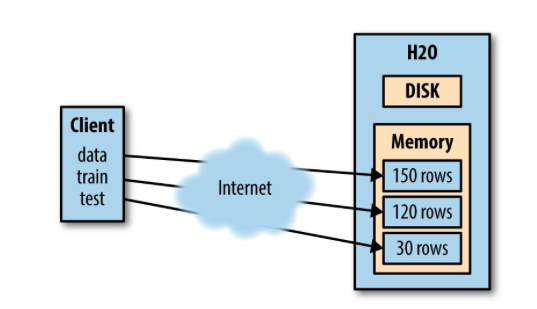
\includegraphics[scale = 0.5,angle = 0]{figure/DataClusters.png}
  \caption[Client and H2O Cluster]{\normalsize{Client and H2O Cluster}}
  \label{fig:HyarnCluster}
  \end{figure}
  
  \section{Apache Spark}\label{apache-spark}
  
  Spark is a big-data platform that provides fast in-memory distributed
  processing. This contrasts with Hadoop, which employs the MapReduce
  processing platform and necessitates data writing to an external disk
  through the Hadoop Distributed File System (HDFS) (Borthakur, n.d.).
  Spark uses the Resilient Distributed Datasets (RDD) data structure,
  which divides the dataset in logical partitions each of which can be
  processed on separate nodes within clusters. This RDD structure obviates
  the need to write data to an external storage system thus providing
  faster in-memory processing (``Spark programming guide,'' n.d.).
  Moreover Apache Spark is an in-memory data processing tool that hosts
  the Spark platform on Apache Hadoop YARN providing a collective and
  shared access to a dataset.
  
  In R, the sparklyr package provides an R interface for Apache Spark.
  Besides a dplyr background, this facilitates the use of Spark's
  distributed machine learning library.
  
  \section{Sparkling Water}\label{sparkling-water}
  
  Sparkling water combines the machine learning capabilities of H2O with
  the in-memory distributed, fast computation of the Spark platform.
  Tachyon, which is an in-memory distributed file system, facilitates
  exchange of data between Spark and H2O (Ambati, n.d.). The rsparkling
  package in R provides access to H2O's machine learning routines within
  the Spark platform accessible over R. Spark data frames can be converted
  to H2O frames thus facilitating machine learning algorithms.
  
  \section{RSparkling}\label{rsparkling}
  
  The rsparkling package facilitates data transfer between Spark and H2O
  dataframes. Rsparkling also allows access to Sparkling Water spark
  package's machine learning algorithms (``Sparkling water (h20) machine
  learning,'' n.d.).
  
  \section{Hadoop YARN}\label{hadoop-yarn}
  
  Apache Hadoop YARN includes separate resource management and job
  scheduling infrastructures in collective resource manager and individual
  node manager through a master-slave hierarchy (as shown by
  \autoref{fig:Hyarn}(``Spark programming guide,'' n.d.)). The
  per-application based application masters negotiate resources with the
  resource manager and execute and monitor tasks through a collaboration
  with the node managers. The resource managers additionally contain a
  scheduler that schedules jobs based on resource requirements. Individual
  node managers are responsible for launching application containers and
  examining resource usage (like memory and disk consumption). These
  updates are then reported back to the resource manager. Per-node
  application master negotiate resource containers with scheduler (Murthy,
  2012).
  
  \begin{figure}[htbp]
  \centering
  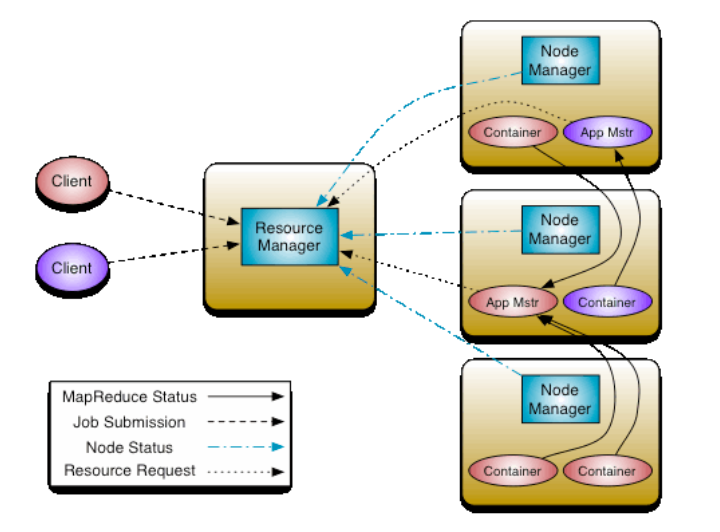
\includegraphics[scale = 0.5,angle = 0]{figure/yarn.png}
  \caption[Hadoop YARN architecture]{\normalsize{Hadoop YARN architecture}}
  \label{fig:Hyarn}
  \end{figure}
  
  \section{Additional Resources}\label{additional-resources}
  
  \begin{itemize}
  \item
    H2O Installation guide -
    \url{http://h2o-release.s3.amazonaws.com/h2o/rel-turing/6/index.html\#R}
  \item
    H2O Documentation -
    \url{http://h2o-release.s3.amazonaws.com/h2o/rel-lambert/5/docs-website/index.html}
  \item
    Sparkling Water Installation -
    \url{http://www.h2o.ai/download/sparkling-water/}
  \item
    Sparkling Water Overview - \url{http://spark.rstudio.com/h2o.html}
  \item
    Sparklyr Overview and Installation - \url{http://spark.rstudio.com}
  \end{itemize}
  
  \chapter{Shiny Explorations}\label{shiny-explorations}
  
  \section{Introduction}\label{introduction-1}
  
  For this analysis, I used the Flights dataset from the United States
  Department of Transportation Bureau of Transportation Statistics. Data
  was set up in the YARN-client cluster in the Hadoop server from years
  2008-2016. Initially it contained variables like year, month and day of
  the trip, departure delay, arrival delay, carrier, tailnumber, distance
  covered, flight number, flight origin, destination and scheduled flight
  time. Additional predictors were created to better gauge the departure
  delay. These variables included day of week, season and weekend status
  and hour of flight delay.
  
  \section{Web Scraping}\label{web-scraping}
  
  Since carrier, plane origin and destination airport information was
  provided as two and three letter code names, following the guidelines
  set by the International Air Transport Association (IATA), additional
  data was scraped from web to include the origin and destination airport
  information as well as the carrier and state names. This data was then
  merged with the flights dataset. Data scraping was performed using rvest
  package and the SelectorGadget tool, a Chrome extension that allows for
  easy CSS webpage selection (see Appendix 2 for complete scraping code).
  
  \section{Shiny App}\label{shiny-app}
  
  Shiny App was used for initial exploratory analysis. Graphical, tabular
  and weather analysis was performed. In addition, networks were
  constructed to visualize number of flights and departure delays between
  airports. Images from the shiny app are shown below each commentary. The
  app itself can be accessed at
  \url{https://r.amherst.edu/apps/ajavaid17/Comps2017Flights/FlightsExpo/}
  (wait time of about half a minute and ignore red ` errors).
  
  \subsection{Graphical Analysis}\label{graphical-analysis}
  
  Graphical shiny analysis was performed on flights with departure delays
  greater than 90 minutes. About 1590467 flights satistied this criterion
  and were used for analysis. Departure delays were analyzed graphically
  by carrier, month, hour, week and weekend status predictors. Mean
  departure delay was computed by averaging the departure delay in minutes
  over the user specified year and carrier, month, hour, week or weekend
  status predictors. The package ggplot2 was used for graphical analysis
  and reactivity was employed to add dynamicity to the graphs. An example
  shiny output of changes in mean departure delay from 2008 to 2016
  grouped by weekend is shown by \autoref{fig:shiny1}.
  
  \begin{figure}[htbp]
  \centering
  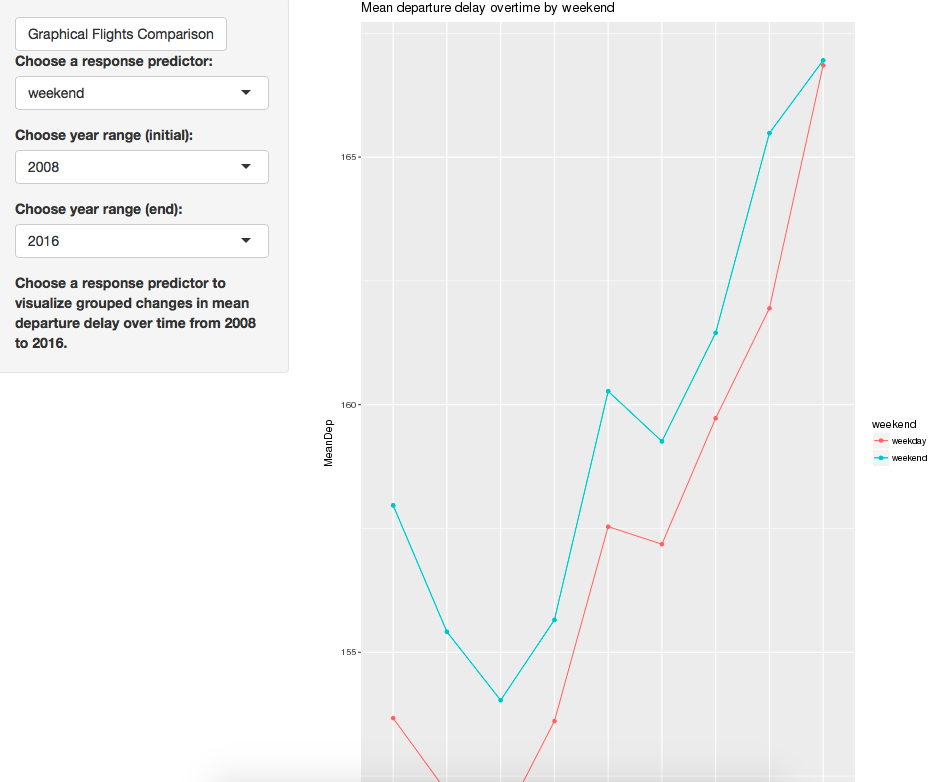
\includegraphics[scale = 0.5,angle = 0]{figure/AppFlights1.png}
  \caption[Graphical Analysis]{\normalsize{Graphical Analysis}}
  \label{fig:shiny1}
  \end{figure}
  
  \subsubsection{Departure delay by
  carrier:}\label{departure-delay-by-carrier}
  
  According to the carrier graphical analysis, Hawaiian airlines had a
  consistently higher delay in comparison to other airlines from
  2008-2016. Hawaiian also experienced the most fluctuations in the
  average departure delays. Southwest and US Air had lowest delays. The
  overall trend though points to slightly increased departure delays from
  2008 to 2016.
  
  \subsubsection{Departure delay by
  month/seasons:}\label{departure-delay-by-monthseasons}
  
  Graphically, differences in departure delay by month appeared to be
  indistinguishable. To better differentiate the delays by month, season
  variable was created. Delays for summer appear to be slightly higher
  than the delays for fall, spring and winter from years 2008 to 2012. The
  general trend points to an increased delay from 2008 to 2016.
  
  \subsubsection{Departure delay by hour/time of day
  status:}\label{departure-delay-by-hourtime-of-day-status}
  
  Hours 0-4 (12 am to 4 am) appeared to be most unpredictable in mean
  departure delay. In comparison, mean departure delay seemed to stablize
  after 2 pm continuing in the evening hours. Though there was a slight
  delay in the evening hours, it did not appear to be as problematic as
  the early morning hour delays.
  
  \subsubsection{Departure delay by
  week/weekend:}\label{departure-delay-by-weekweekend}
  
  Differences in mean departure delay appeared to be indistinguishable by
  week status. In comparison, there appeared to be higher delays on
  weekends than weekdays.
  
  \clearpage
  
  \subsection{Tabular Analysis}\label{tabular-analysis}
  
  The tabular analysis showed the mean departure delay for all flights for
  the specified origin and destination states. In addition, the panel
  showed departure delays for all flights for the user selected origin and
  destination airports. Data Table was used which provided searching
  functionalities to the app. An output of flights from New York to
  California from the shiny app for the tabular analysis section is shown
  by \autoref{fig:shiny2}.
  
  \begin{figure}[htbp]
  \centering
  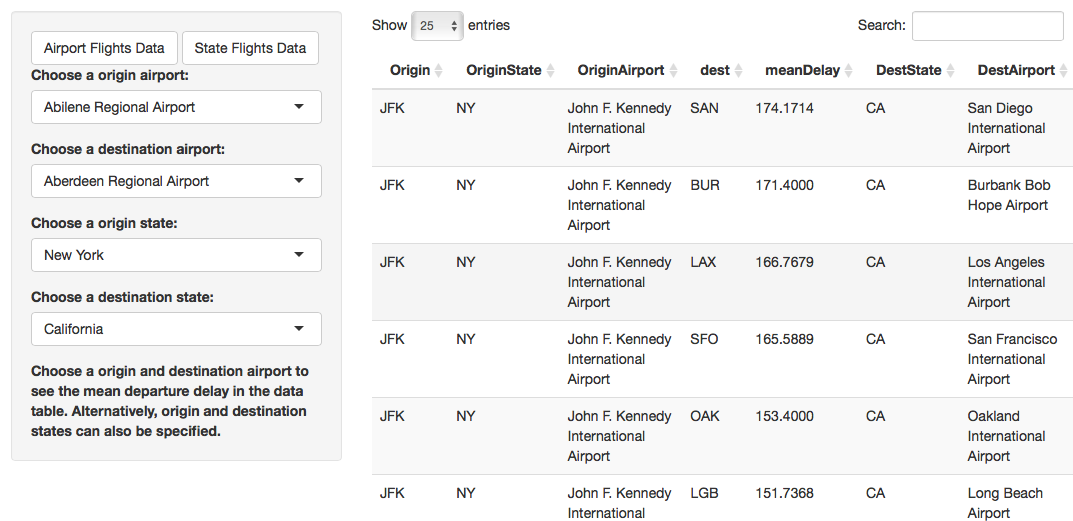
\includegraphics[scale = 0.4,angle = 0]{figure/Shiny2.png}
  \caption[Tabular Analysis]{\normalsize{Tabular Analysis}}
  \label{fig:shiny2}
  \end{figure}
  
  \clearpage
  
  \subsection{Graphical Weather
  Analysis}\label{graphical-weather-analysis}
  
  In addition to the general analysis for all flights with departure
  delays greater than 90 minutes from 2008 to 2016, analysis was performed
  to gauge the effect of weather on total delay, quantified by sum of
  departure and arrival delays for LaGuardia, John F. Kennedy and Newark
  Liberty International Airport. Weather analysis was only performed for
  2013 since data for this year was readily available in the nycflights13
  package. In comparison, weather analysis from 2008 to 2016 would have
  entailed possible pipeline constructions to fetch data from the National
  Climatic Data Center (NOAA) by the timestamp specified by the flights
  data in the Hadoop clusters, a project pursued in subsequent work. The
  weather data from the nycflights13 package contained about 135059
  observations. Effect of weather metrics like temperature, dewpoint,
  humidity, wind direction, wind speed, wind gust, precipitation, pressure
  and visibility was analyzed on the total delay over measures like week,
  weekend, month and seasons. An output from the shiny app is shown in
  \autoref{fig:shiny3} depicting changes in total delay by temperature and
  weekend status.
  
  \begin{figure}[htbp]
  \centering
  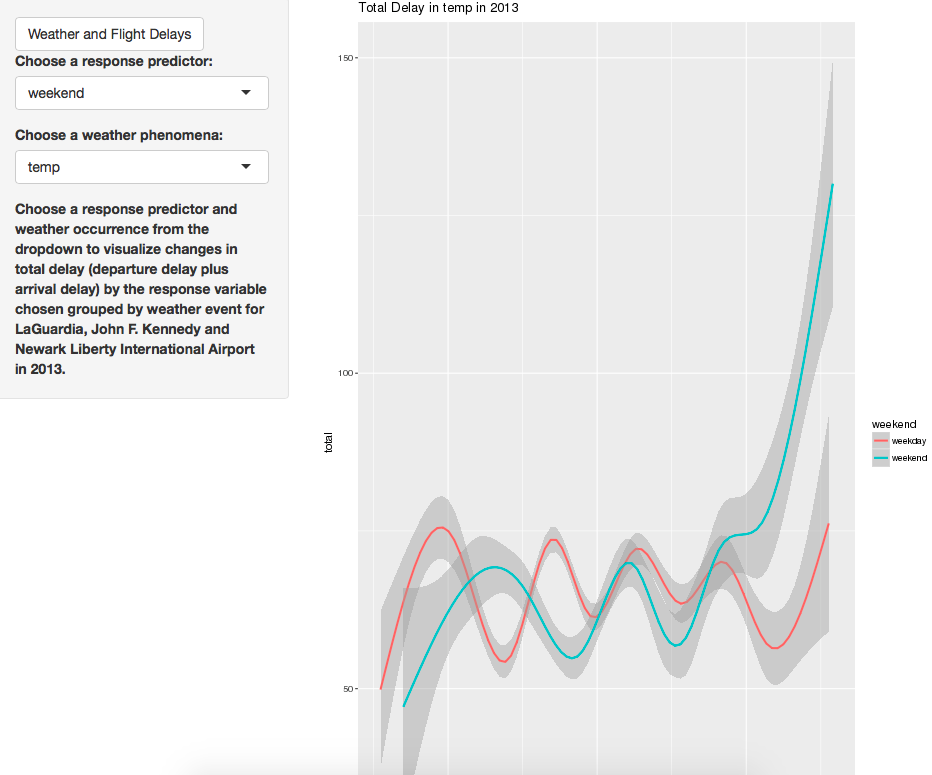
\includegraphics[scale = 0.5,angle = 0]{figure/AppImage2.png}
  \caption[Weather Analysis]{\normalsize{Weather Analysis}}
  \label{fig:shiny3}
  \end{figure}
  
  \subsubsection{Total delay by week and
  weather:}\label{total-delay-by-week-and-weather}
  
  Total delay did not show considerable changes by temperature over the
  weeks besides a rise in departure delay on Friday with low temperature
  and a rise in departure delay on Sunday with increase in temperature.
  Similarly there did not appear to be a visible pattern in total delay by
  weather patterns over day of week. A general trend pointed towards an
  increase in total delay with visibility and a decrease in total delay
  with increased pressure. Increase in humidity appeared to increase
  departure delay. While Saturday experienced a decrease in total delay
  with an increase in humidity, this decrease was not necessarily
  particularly distinguished to be commented on.
  
  \subsubsection{Total delay by weekend and
  weather:}\label{total-delay-by-weekend-and-weather}
  
  There appeared to be a higher increase in total delay with an increase
  in temperature on a weekend than a weekday. This higher increase in
  total delay was also visible with an increase in dewpoint and
  precipitation on weekends than weekdays. In comparison, increase in
  total delay on a weekday than weekends with an increase in humidity is
  apparent. Decrease in total delay with an increase in pressure and
  visibility was apparent for both weekdays and weekends. For low
  temperatures, dewpoint, precipitation, humidity, pressure and
  visibility, differences in weekday and weekends total delays do not
  appear to be distinguishable.
  
  \subsubsection{Total delay by month and
  weather:}\label{total-delay-by-month-and-weather}
  
  December experienced higher total delays with an increase in temperature
  in comparison to other months. Differences in total delay with respect
  to humidity appeared to be indistinguishable by month. Increase in
  humidity seemed to produce a higher increase in total delay for March,
  February and December in comparison to other months. There did not
  appear to be considerable changes in total delays by pressure over the
  months were not observed though there was a presence of a general trend
  towards decreased total delay with an increase in pressure.
  
  \subsubsection{Total delay by season and
  weather:}\label{total-delay-by-season-and-weather}
  
  In regards to seasonal variations, there appeared to be a higher
  increase in total delays with an increase in temperature during winter
  than during fall and spring. Increase in dewpoint produced a higher
  increase in total delays for February and March than for other months.
  Differences in total delay by month did not appear to be distinguishable
  for pressure and humidity measures. Overall trend pointed to an increase
  in total delay with an increase in humidity and a decrease in total
  delay with an increase in pressure for all months.
  
  \clearpage
  
  \subsection{Flights Network Analysis}\label{flights-network-analysis}
  
  Fourth panel in shiny showed a network of randomly sampled 500 flights
  with their destination and origin airports specified as vertices and the
  width of the edges representing the extent of the departure delay. The
  network only included flights with delays greater than 90 minutes.
  Airports can be highilghted on the network from the dropdown menu. In
  addition, the data table for the network was shown which could be
  queried for the numerically exact departure delay. This graph was
  constructed with igraph and the visnetwork package. The departure delays
  were normalized to show appropriate scaling. An output from shiny for a
  random network as well as the associated data table is shown by
  \autoref{fig:shiny4}.
  
  \begin{figure}[htbp]
  \centering
  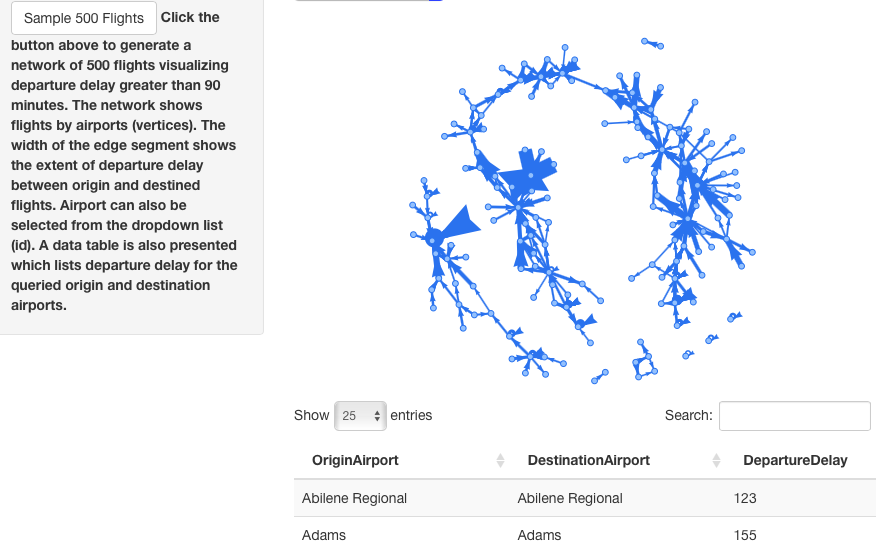
\includegraphics[scale = 0.5,angle = 0]{figure/Shiny4.png}
  \caption[Flights Network]{\normalsize{Flights Network}}
  \label{fig:shiny4}
  \end{figure}
  
  \clearpage
  
  \subsection{Mapping Flights}\label{mapping-flights}
  
  Last shiny panel showed the mean departure delay by airport from 2008 to
  2016 in the United States for all flights with departure delay greater
  than 90 minutes. Hovering over the points displayed the state, airport
  as well as the average departure delay for that airport. From the graph,
  Wyoming Cheyenne Regional Airport appeared to have a visibly high mean
  departure delay of 247.71 minutes. Other airports with high departure
  delay included Greater Rockford Airport in Illinois with a mean
  departure delay of 240.22 minutes and Bemidji Regional Airport in
  Minnesota with mean departure delay of 235.76 minutes. Overall trend
  pointed to low departure delays along the West coast. An output from the
  shiny app is shown by \autoref{fig:shiny5}.
  
  \begin{figure}[htbp]
  \centering
  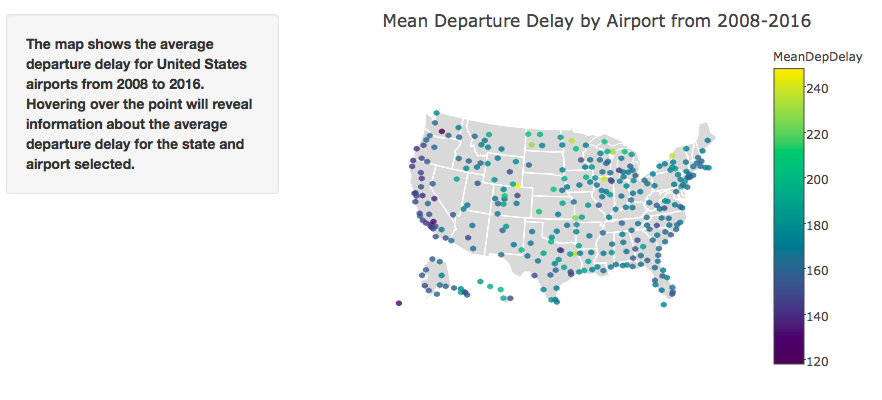
\includegraphics[scale = 0.5,angle = 0]{figure/Shiny5.png}
  \caption[Maps Analysis]{\normalsize{Maps Analysis}}
  \label{fig:shiny5}
  \end{figure}
  
  \clearpage
  
  \chapter{Logistical Reasoning}\label{logistical-reasoning}
  
  \section{Introduction}\label{introduction-2}
  
  H2O platform was used to construct a logistic model to predict
  occurrence of departure delay over 20 minutes from 2008 to 2016. Delay
  of 30 minutes was chosen since it provided adequate sample for flights
  both experiencing and not experiencing departure delay. Analysis was
  performed on a random sample of 200000 observations. This size was
  easily transferable to the Spark environment while larger sample sizes
  crashed the server. Occurrence of delay over 30 minutes was assessed
  against year, arrival delay, carrier, air time, distance, week and
  season predictors. Initially, hour, month and weekend status predictors
  were also used to estimate the incidence of delay though they appeared
  to have no importance and therefore were not used in subsequent
  analysis.
  
  \section{H2O Connection}\label{h2o-connection}
  
  After the installation process, h2o.init() was used to establish H2O
  connection to local host at port 54321. Default connection is
  established with 1GB of memory. Additionl cluster memory can be
  allocated with max\_mem\_size specification. Since this project was
  performed using the Apache Spark platform, connection with YARN Hadoop
  cluster was established. This connection entailed a cluster
  initialization in the shell followed by a Spark connection as shown
  below.
  
  \begin{Shaded}
  \begin{Highlighting}[]
  \KeywordTok{library}\NormalTok{(sparklyr)}
  \KeywordTok{library}\NormalTok{(rsparkling)}
  \KeywordTok{library}\NormalTok{(dplyr)}
  \KeywordTok{options}\NormalTok{(}\DataTypeTok{rsparkling.sparklingwater.version =} \StringTok{"1.6.8"}\NormalTok{)}
  
  \CommentTok{#Initialize a cluster (without Hadoop connection)}
  \KeywordTok{h2o.init}\NormalTok{()}
  
  \CommentTok{#Connect to YARN through shell}
  \KeywordTok{kinit}\NormalTok{()}
  \NormalTok{klist  }
  
  \CommentTok{#Connect to Apache Spark Hadoop in markdown }
  \NormalTok{sc <-}\StringTok{ }\KeywordTok{spark_connect}\NormalTok{(}\DataTypeTok{master =} \StringTok{"yarn-client"}\NormalTok{)}
  \end{Highlighting}
  \end{Shaded}
  
  \section{Spark Data Integration}\label{spark-data-integration}
  
  Once the connection was estabished, flights dataset was created (see
  Appendix 2 for full details on the dataset creation). Final flights
  dataset creation involved copying data from Hadoop to Spark environment
  from 2008 to 2016. The dataset columns were then renamed. The final
  dataset was saved in HadoopLogMod.Rda and copied in the Spark
  environment with subsequent use. Data copy process from Hadoop to Spark
  is shown below. If a local connection was established instead of Hadoop,
  R data frame can be converted to H2OFrame using the as.h2o command.
  
  \begin{Shaded}
  \begin{Highlighting}[]
  \CommentTok{#If connection is established to Hadoop:}
  \KeywordTok{load}\NormalTok{(}\StringTok{"HadoopLogMod.Rda"}\NormalTok{)}
  \KeywordTok{set.seed}\NormalTok{(}\DecValTok{134}\NormalTok{)}
  \NormalTok{sample <-}\StringTok{ }\NormalTok{FullDatLog[}\KeywordTok{sample}\NormalTok{(}\KeywordTok{nrow}\NormalTok{(FullDatLog), }
                                \DecValTok{200000}\NormalTok{, }\DataTypeTok{replace =} \OtherTok{FALSE}\NormalTok{, }
                                \DataTypeTok{prob =} \OtherTok{NULL}\NormalTok{),]}
  \NormalTok{LogDataMod <-}\StringTok{ }\KeywordTok{copy_to}\NormalTok{(sc, sample, }\StringTok{"LogData"}\NormalTok{, }
                        \DataTypeTok{overwrite =} \OtherTok{TRUE}\NormalTok{)  }
  
  
  \CommentTok{#If no connection established to Hadoop: }
  \CommentTok{#Read from local file}
  \NormalTok{FlightsDat =}\StringTok{ }\KeywordTok{h2o.importFile}\NormalTok{(localH2O, }\DataTypeTok{path =} \NormalTok{prosFlights)}
  \CommentTok{#Convert to h2o data frame}
  \NormalTok{FlightsDat <-}\StringTok{ }\KeywordTok{as.h2o}\NormalTok{(sample)}
  \end{Highlighting}
  \end{Shaded}
  
  \section{Data Partitioning}\label{data-partitioning}
  
  After the data was copied in the Spark environment, it was partitioned
  in test and training sets. A 75/25 partition was used as shown below
  where training set had about 75\% of the data (149789 observations) and
  test set had about 25\% (50211 observations). The partition was not
  strictly 75/25 since the split is not performed exactly.
  
  \begin{Shaded}
  \begin{Highlighting}[]
  \CommentTok{#Partitioning data frame in Spark }
  \NormalTok{partitions <-}\StringTok{ }\NormalTok{LogDataMod %>%}
  \StringTok{  }\KeywordTok{sdf_partition}\NormalTok{(}\DataTypeTok{training =} \FloatTok{0.75}\NormalTok{, }\DataTypeTok{test =} \FloatTok{0.25}\NormalTok{, }\DataTypeTok{seed =} \DecValTok{1099}\NormalTok{)}
  
  \CommentTok{#Partitioning data locally within the H2O platform}
  \NormalTok{splits <-}\StringTok{ }\KeywordTok{h2o.splitFrame}\NormalTok{(LogDataMod, }\KeywordTok{c}\NormalTok{(}\FloatTok{0.75}\NormalTok{,}\FloatTok{0.25}\NormalTok{), }\DataTypeTok{seed=}\DecValTok{1099}\NormalTok{)}
  \end{Highlighting}
  \end{Shaded}
  
  \section{Checking Conditions}\label{checking-conditions}
  
  Since the response (dep\_delayIn) was a binary predictor indicating the
  incidence of departure delay of 30 minutes, linearity was assumed.
  Randomness and independence may not necessarily be valid assumptions
  since typically a late flight results in subsequent delays. Analysis of
  the randomness and independence assumption will require tracking flight
  schedules from 2008 to 2016. Future studies could assess this
  assumption. This study proceeded with caution.
  
  \section{Modeling}\label{modeling}
  
  Once the data was partitioned in test and training sets, logistic
  regression model was specifed as shown. The setdiff command took the set
  difference between predictors in the training dataset and the set of
  predictors specified in the command (dep\_DelayIn, orig\_id, hour,
  month, weekend). The h2o.glm function can be used to specify a binomial
  family function. Additional arguments in the h2o.glm function include
  nfolds (specifies the number of folds for cross validation), alpha (0-1
  numeric that specifies the elastic-net mixing parameter, set to ensure
  regularization and consequently prevent overfitting), lambda (specifies
  a non-negative shrinkage parameter) and lambda\_search (logical
  indicating whether or not search is conducted over the lambda space
  specified). In addition, h2o models can be stopped early with
  specification of stopping metrics like misclassification error, rsquared
  and mean squared error. Every model has an associated model id which can
  be referenced for future model iterations. In the model below, a 5-fold
  cross validation was performed with alpha level of 0.1. As mentioned
  above, the logistic model below attempted to predict the occurrence of
  departure delay by variables including year, arrival delay, carrier, air
  time, distance, week and season.
  
  \begin{Shaded}
  \begin{Highlighting}[]
  \NormalTok{myX =}\StringTok{ }\KeywordTok{setdiff}\NormalTok{(}\KeywordTok{colnames}\NormalTok{(training), }\KeywordTok{c}\NormalTok{(}\StringTok{"dep_delayIn"}\NormalTok{, }
                                      \StringTok{"orig_id"}\NormalTok{, }\StringTok{"hour"}\NormalTok{, }
                                      \StringTok{"month"}\NormalTok{, }\StringTok{"weekend"}\NormalTok{))}
   
  \NormalTok{regmod <-}\StringTok{ }\KeywordTok{h2o.glm}\NormalTok{(}\DataTypeTok{y =} \StringTok{"dep_delayIn"}\NormalTok{, }\DataTypeTok{x =} \NormalTok{myX, }
                    \DataTypeTok{training_frame =} \NormalTok{training, }\DataTypeTok{family =} \StringTok{"binomial"}\NormalTok{,}
          \DataTypeTok{alpha =} \FloatTok{0.1}\NormalTok{, }\DataTypeTok{lambda_search =} \OtherTok{FALSE}\NormalTok{, }\DataTypeTok{nfolds =} \DecValTok{5}\NormalTok{)}
  \end{Highlighting}
  \end{Shaded}
  
  \section{Model Assessment}\label{model-assessment}
  
  Model performance was assessed with the h2o.performance function, which
  provides access to evaluation metrics like MSE, RMSE, LogLoss, AUC and
  \(R^{2}\). The \(R^{2}\) for this model was 0.710 and the AUC was 0.987
  as shown by \autoref{fig:Hyarn20}. The \(R^{2}\) value indicated that
  about 71\% of the variation in departure delay was accounted for by
  predictors year, arrival delay, carrier, air time, distance, week and
  season. In addition to the h2o.performance function, h2o.auc and
  h2o.confusionMatrix (see \autoref{fig:Hyarn26}) was used to retrieve the
  analogous parameters. The AUC curve was visualized as shown by figure
  \autoref{fig:Hyarn48} with the plot(h2o.performance) command.
  
  \begin{Shaded}
  \begin{Highlighting}[]
  \KeywordTok{h2o.performance}\NormalTok{(regmod) }
  \KeywordTok{h2o.auc}\NormalTok{(regmod) }
  \KeywordTok{h2o.confusionMatrix}\NormalTok{(regmod) }
  \NormalTok{accuracy <-}\StringTok{ }\NormalTok{(mat$No[}\DecValTok{1}\NormalTok{]+mat$Yes[}\DecValTok{2}\NormalTok{])/(mat$No[}\DecValTok{1}\NormalTok{]+}
  \StringTok{                                      }\NormalTok{mat$No[}\DecValTok{2}\NormalTok{]+mat$Yes[}\DecValTok{1}\NormalTok{]+}
  \StringTok{                                      }\NormalTok{mat$Yes[}\DecValTok{2}\NormalTok{]) }
  \KeywordTok{plot}\NormalTok{(}\KeywordTok{h2o.performance}\NormalTok{(regmod)) }\CommentTok{#plot the auc curve }
  \end{Highlighting}
  \end{Shaded}
  
  \begin{figure}[htbp]
  \centering
  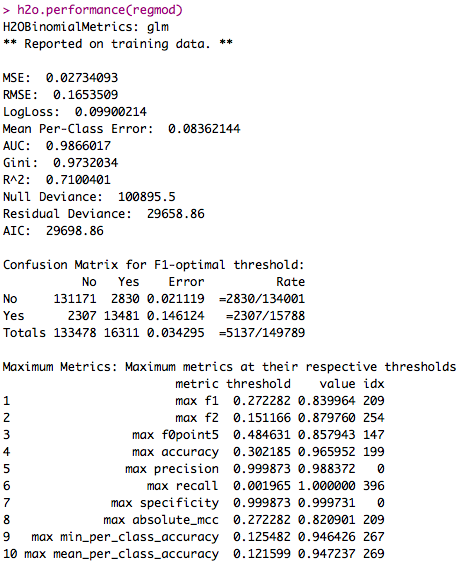
\includegraphics[scale = 0.7,angle = 0]{figure/PerformanceLogMod.png}
  \caption[Model Performance]{\normalsize{Model Performance}}
  \label{fig:Hyarn20}
  \end{figure}
  
  \begin{figure}[htbp]
  \centering
  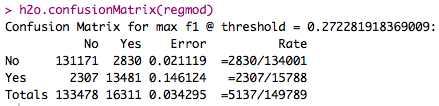
\includegraphics[scale = 0.8,angle = 0]{figure/confMatLog.png}
  \caption[Confusion Matrix]{\normalsize{Confusion Matrix}}
  \label{fig:Hyarn26}
  \end{figure}
  
  \begin{figure}[htbp]
  \centering
  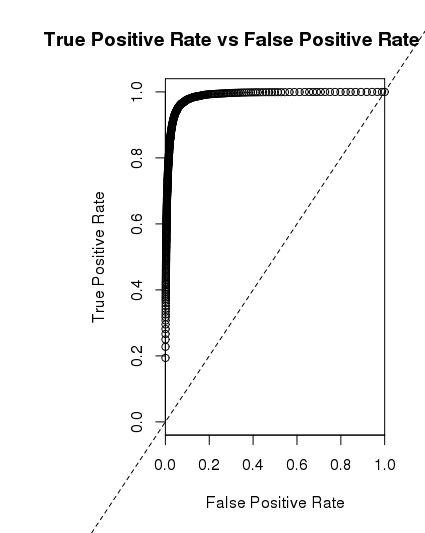
\includegraphics[scale = 0.8,angle = 0]{figure/ROCCurveLog-3.png}
  \caption[AUC Curve]{\normalsize{AUC Curve}}
  \label{fig:Hyarn48}
  \end{figure}
  
  \clearpage
  
  As the variable importance plot in \autoref{fig:Hyarn34} shows, arrival
  delay was most important in predicting the occurrence of departure
  delays greater than 30 minutes. Arrival delay was followed by air time
  and distance predictors. Air time appears to be a negative predictor of
  delay indicating that flights with high air time appear less likely to
  experience departure delays greater than 30 minutes. In comparison,
  flights that cover more distance are more likely to experience departure
  delays greater than 30 minutes. Southwest (WN) and United Airlines (UA)
  were more important at predicting departure delays greater than 30
  minutes while US Airways (US) did not. Year 2008 and 2009 negatively
  predicted departure delays greater than 30 minutes while year 2015
  appeared to be more likely to experience departure delays greater than
  30 minutes. In comparison, summer appeared to be an important season for
  predicting departure delay greater than 30 minutes.
  
  \begin{Shaded}
  \begin{Highlighting}[]
  \KeywordTok{h2o.varimp}\NormalTok{(regmod) }\CommentTok{#compute variable importance}
  \KeywordTok{h2o.varimp_plot}\NormalTok{(regmod) }\CommentTok{#plot variable importance}
  \end{Highlighting}
  \end{Shaded}
  
  \begin{figure}[htbp]
  \centering
  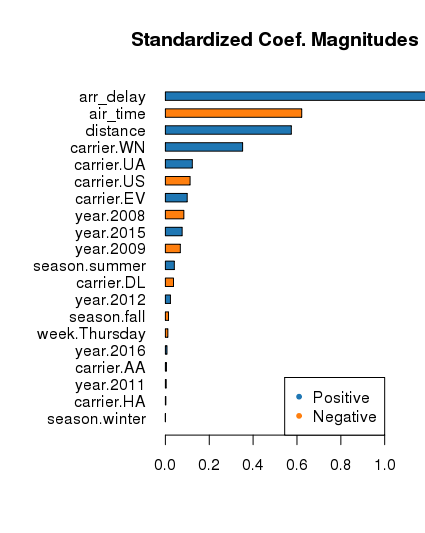
\includegraphics[scale = 1,angle = 0]{figure/VarImpPlot-3.png}
  \caption[Variable Importance]{\normalsize{Variable Importance}}
  \label{fig:Hyarn34}
  \end{figure}
  
  \clearpage
  
  \section{Making Predictions}\label{making-predictions}
  
  After model assessments were analyzed, predictions can be performed on
  the test set. The accuracy of the test set was calculated and compared
  with the accuracy of the cross-validated training set. In this case,
  accuracy of the test set of 0.967 compares with the accuracy of the
  training data of 0.966. Since the error rates are similar, occurrence of
  overfitting was reduced. In addition to comparing the accuracy of the
  test with the training set, accuracy of the training data can also be
  compared with the accuracy of the validation data (see Deep Learning).
  
  \begin{Shaded}
  \begin{Highlighting}[]
  \NormalTok{pred <-}\StringTok{ }\KeywordTok{h2o.performance}\NormalTok{(}\DataTypeTok{object =} \NormalTok{regmod, }\DataTypeTok{newdata =} \NormalTok{test) }
  \KeywordTok{mean}\NormalTok{(pred$predict==test$dep_delayIn) }\CommentTok{#accuracy of test set }
  \end{Highlighting}
  \end{Shaded}
  
  \section{Connection Shutdown}\label{connection-shutdown}
  
  The established spark connection was disconnected with the
  spark\_disconnect command as shown below.
  
  \begin{Shaded}
  \begin{Highlighting}[]
  \KeywordTok{spark_disconnect}\NormalTok{(sc) }\CommentTok{#disconnect the spark session }
  \KeywordTok{h2o.shutdown}\NormalTok{(}\DataTypeTok{prompt=}\OtherTok{FALSE}\NormalTok{) }\CommentTok{#close the H2O connection }
  \end{Highlighting}
  \end{Shaded}
  
  \section{Conclusion}\label{conclusion}
  
  This chapter discussed concepts like connecting to local or YARN
  connection, partitioning datasets and performing generalized linear
  regression modeling. Additionally model assessments were discussed.
  
  Overall arrival delay appeared to be most important in predicting
  departure delay greater than 30 minutes indicating that flights with
  increased arrival delay may have increased tendency to experience
  departure delay. Air time and distance also appeared to be important in
  predicting occurrence of departure delay greater than 30 minutes. Higher
  air time coverage thus seemed to decrease the occurrence of departure
  delay suggesting that flights that have been flying for a while may have
  less chance of experiencing departure delay. This finding does not seem
  intuitive but it may be the case that if the aircraft is flying for a
  while, it is more adept at handling delays. More distance coverage is
  associated with higher likelihood of departure delay greater than 30
  minutes. Summer also increased chance of departure delay which seems
  intuitive since it is typically a busy season for vacations as well as
  tourist explorations. There also appeared to be an increased likelihood
  of departure delay greater than 30 minutes in more recent years like
  2015 than in 2008 or 2009 which could point to an increased trend in air
  travel resulting in increased traffic and consequently higher likelihood
  of experiencing departure delay.
  
  \chapter{Weathering Logistics}\label{weathering-logistics}
  
  \section{Introduction}\label{introduction-3}
  
  H2O platform was used to construct a logistic model to predict whether
  or not departure delay over 30 minutes can be predicted using weather
  data from nycflights13 package for LaGuardia, John F. Kennedy and Newark
  Liberty International airports in 2013. Analysis was performed on data
  containing 48126 observations. Occurrence of delay over 30 minutes was
  assessed against season, month, week, weekend, day, hour, arrival delay,
  distance and air time. Weather predictors included temperature,
  dewpoint, humidity, wind direction, wind speed, wind gust,
  precipitation, pressure and visibility.
  
  \section{Data Partitioning}\label{data-partitioning-1}
  
  After the data connection was established and data was copied in the
  Spark environment, it was partitioned in test and training sets. A 75/25
  split of training and test data was used. The training data contained
  36153 observations and test set contained 11973 observations.
  
  \begin{Shaded}
  \begin{Highlighting}[]
  \KeywordTok{library}\NormalTok{(sparklyr)}
  \KeywordTok{library}\NormalTok{(rsparkling)}
  \KeywordTok{library}\NormalTok{(dplyr)}
  \KeywordTok{options}\NormalTok{(}\DataTypeTok{rsparkling.sparklingwater.version =} \StringTok{"1.6.8"}\NormalTok{)}
  \NormalTok{sc <-}\StringTok{ }\KeywordTok{spark_connect}\NormalTok{(}\DataTypeTok{master =} \StringTok{"yarn-client"}\NormalTok{)}
  \KeywordTok{load}\NormalTok{(}\StringTok{"flights_weather2.Rda"}\NormalTok{)}
  
  \NormalTok{partitions <-}\StringTok{ }\NormalTok{LogDataMod %>%}
  \StringTok{  }\KeywordTok{sdf_partition}\NormalTok{(}\DataTypeTok{training =} \FloatTok{0.75}\NormalTok{, }\DataTypeTok{test =} \FloatTok{0.25}\NormalTok{, }\DataTypeTok{seed =} \DecValTok{1099}\NormalTok{)}
  
  \CommentTok{#Partitioning data locally within the H2O platform}
  \NormalTok{splits <-}\StringTok{ }\KeywordTok{h2o.splitFrame}\NormalTok{(LogDataMod, }\KeywordTok{c}\NormalTok{(}\FloatTok{0.75}\NormalTok{,}\FloatTok{0.25}\NormalTok{), }\DataTypeTok{seed=}\DecValTok{1099}\NormalTok{)}
  \end{Highlighting}
  \end{Shaded}
  
  \section{Checking Conditions}\label{checking-conditions-1}
  
  Since the response (dep\_delayIn) was a binary predictor indicating the
  incidence of departure delay of 30 minutes, linearity was assumed.
  Randomness and independence may not necessarily be valid assumptions
  since typically a late flight results in subsequent delays but the study
  proceeded with caution.
  
  \section{Modeling}\label{modeling-1}
  
  Logistic model was used as shown below to predict whether or not
  departure delay occurs against predictors season, month, week, weekend,
  day, hour, arrival delay, distance, air time, temprature, dewpoint,
  humidity, wind direction, wind speed, wind gust, precipitation, pressure
  and visibility. The same parameters as the logistic model in the
  previous chapter were used (alpha = 0.1, lambda\_search = FALSE and
  5-folds cross-validation).
  
  \begin{Shaded}
  \begin{Highlighting}[]
  \NormalTok{myX =}\StringTok{ }\KeywordTok{setdiff}\NormalTok{(}\KeywordTok{colnames}\NormalTok{(training), }\KeywordTok{c}\NormalTok{(}\StringTok{"dep_delayIn"}\NormalTok{)) }\CommentTok{#set difference}
   
  \NormalTok{regmodWeather <-}\StringTok{ }\KeywordTok{h2o.glm}\NormalTok{(}\DataTypeTok{y =} \StringTok{"dep_delayIn"}\NormalTok{, }\DataTypeTok{x =} \NormalTok{myX, }
                    \DataTypeTok{training_frame =} \NormalTok{training, }\DataTypeTok{family =} \StringTok{"binomial"}\NormalTok{,}
          \DataTypeTok{alpha =} \FloatTok{0.1}\NormalTok{, }\DataTypeTok{lambda_search =} \OtherTok{FALSE}\NormalTok{, }\DataTypeTok{nfolds =} \DecValTok{5}\NormalTok{)}
  \end{Highlighting}
  \end{Shaded}
  
  \section{Model Assessment}\label{model-assessment-1}
  
  Model performance was assessed with h2o.performance. \(R^{2}\) for this
  model was 0.616 and the AUC was 0.945 as shown by \autoref{fig:weath1}.
  The \(R^{2}\) value indicated that about 61\% of the variation in the
  departure delay variable was accounted for by season, month, week,
  weekend, day, hour, arrival delay, distance, air time, temprature,
  dewpoint, humidity, wind direction, wind speed, wind gust,
  precipitation, pressure and visibility. Value of 0.61 compared with an
  \(R^{2}\) of 0.71 for the logistic model without weather consideration.
  In addition to the h2o.performance function, h2o.confusionMatrix (see
  \autoref{fig:weath2}) was used to retrieve the confusion matrix. The AUC
  curve was visualized as shown by figure \autoref{fig:weath3} with the
  plot(h2o.performance) command.
  
  \begin{Shaded}
  \begin{Highlighting}[]
  \KeywordTok{h2o.performance}\NormalTok{(regmodWeather) }
  \KeywordTok{h2o.auc}\NormalTok{(regmodWeather) }
  \KeywordTok{h2o.confusionMatrix}\NormalTok{(regmod) }
  \NormalTok{accuracy <-}\StringTok{ }\NormalTok{(mat$No[}\DecValTok{1}\NormalTok{]+mat$Yes[}\DecValTok{2}\NormalTok{])/(mat$No[}\DecValTok{1}\NormalTok{]+}
  \StringTok{                                      }\NormalTok{mat$No[}\DecValTok{2}\NormalTok{]+mat$Yes[}\DecValTok{1}\NormalTok{]+}
  \StringTok{                                      }\NormalTok{mat$Yes[}\DecValTok{2}\NormalTok{]) }
  \KeywordTok{plot}\NormalTok{(}\KeywordTok{h2o.performance}\NormalTok{(regmodWeather)) }\CommentTok{#plot the auc curve }
  \end{Highlighting}
  \end{Shaded}
  
  \begin{figure}[htbp]
  \centering
  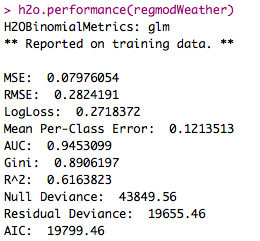
\includegraphics[scale = 0.7,angle = 0]{figure/regmodPerformWeather.png}
  \caption[Model Performance]{\normalsize{Model Performance}}
  \label{fig:weath1}
  \end{figure}
  
  \begin{figure}[htbp]
  \centering
  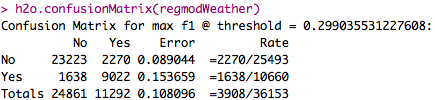
\includegraphics[scale = 0.8,angle = 0]{figure/regModWeather2.png}
  \caption[Confusion Matrix]{\normalsize{Confusion Matrix}}
  \label{fig:weath2}
  \end{figure}
  
  \begin{figure}[htbp]
  \centering
  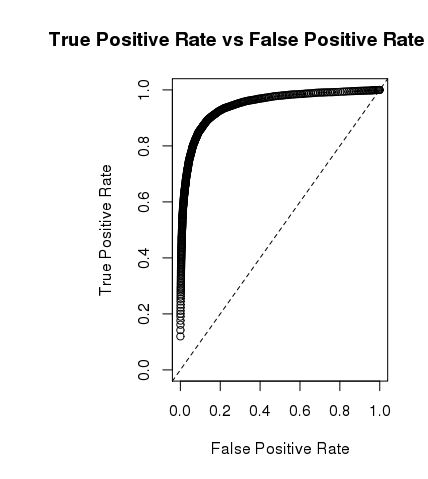
\includegraphics[scale = 0.8,angle = 0]{figure/AUCWeather.png}
  \caption[AUC Curve]{\normalsize{AUC Curve}}
  \label{fig:weath3}
  \end{figure}
  
  \clearpage
  
  As the variable importance plot in \autoref{fig:weath4} shows, arrival
  delay, air time and distance were all important in predicting departure
  delay greater than 30 minutes. While arrival delay and distance
  positively predicted the occurrence of departure delay, meaning an
  increase in these variables was linked with the occurrence of delay,
  distance negatively predicted delay meaning an increase in distance made
  the occurrence of departure delay greater than 30 minutes less likely.
  Day 8 of the month along with hour 6 (6 am) and 8 (8 am) were also
  negatively linked with the occurrence of departure delay greater than 30
  minutes. Additionally American Eagle (MQ), day 14 and Tuesday were
  negatively associated with departure delay. Hours 19 (7 pm), 21 (9 pm)
  and 20 (8 pm) were positively linked with delay. Temperature and wind
  direction appeared to be the only two important weather predictors in
  the top 30 variable important plot shown. Both temperature and wind
  direction are positively associated meaning increase in these predictors
  is linked with increased likelihood of the occurrence of departure delay
  greater than 30 minutes.
  
  \begin{Shaded}
  \begin{Highlighting}[]
  \KeywordTok{h2o.varimp}\NormalTok{(regmodWeather) }\CommentTok{#compute variable importance}
  \KeywordTok{h2o.varimp_plot}\NormalTok{(regmodWeather) }\CommentTok{#plot variable importance}
  \end{Highlighting}
  \end{Shaded}
  
  \begin{figure}[htbp]
  \centering
  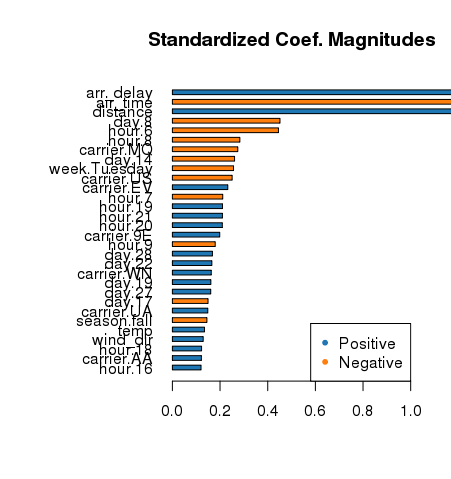
\includegraphics[scale = 1,angle = 0]{figure/top30Weather.png}
  \caption[Variable Importance]{\normalsize{Variable Importance}}
  \label{fig:weath4}
  \end{figure}
  
  \clearpage
  
  \section{Making Predictions}\label{making-predictions-1}
  
  After model assessments were analyzed, predictions were performed on
  test set. The accuracy of the test set was calculated and compared with
  the accuracy of the cross-validated training set. In this case, accuracy
  of the test set of 0.891 compares with the accuracy of the training set
  of 0.893. Since the error rates were similar, occurrence of overfitting
  was reduced.
  
  \begin{Shaded}
  \begin{Highlighting}[]
  \NormalTok{pred <-}\StringTok{ }\KeywordTok{h2o.performance}\NormalTok{(}\DataTypeTok{object =} \NormalTok{regmodWeather, }\DataTypeTok{newdata =} \NormalTok{test) }
  \KeywordTok{mean}\NormalTok{(pred$predict==test$dep_delayIn) }\CommentTok{#accuracy of test set }
  \end{Highlighting}
  \end{Shaded}
  
  \section{Conclusion}\label{conclusion-1}
  
  This chapter incorporated weather gauging predictors in the logistic
  model built in the previous chapter. The intent was to examine the role
  weather metrics like temperature, dewpoint, humidity, wind direction,
  wind speed, wind gust, precipitation, pressure and visibility played in
  predicting departure delay controlling for predictors like arrival
  delay, distance and air time.
  
  Overall arrival delay, distance and air time were the most important
  predictors. Though temperature and wind direction were the only
  important weather predictors, they cannot be considered extremely
  important since they ranked 26th and 27th, respectively. Morover the
  \(R^{2}\) value of the logistic model with the weather variables does
  not appear to improve upon the logistic model built without weather
  predictors in the previous chapter. According to these results, weather
  does not appear to play a large role in predicting departure delay.
  Additional weather data can be collected in the future to further
  examine its role in predicting delays.
  
  \chapter{Deep Learning}\label{deep-learning}
  
  \section{Introduction}\label{introduction-4}
  
  H2O deep learning follows the multi-layer, feedforward neural network
  model (Reddy, n.d.). In the feedforward neural network model, the inputs
  are weighted, combined and transmitted as output signal by the connected
  neuron. Function f shown in \autoref{fig:Hyarn6} shows a nonlinear
  activation function where the bias accounts for the activation threshold
  (Candel, Lanford, LeDell, Parmar, \& Arora, 2015). A nonlinear
  activation function ensures that the linearly input hidden layers
  experience variation. Otherwise the output will simply be a linear
  combination of the hidden layers making the use of hidden layers
  irrelevant. Examples of activation functions include sigmoid and
  rectified linear unit (ReLU). The multi-layer platform consists of
  layers of interconnected neurons that is initiated with the input layer
  followed by layers of nonlinearity culminating in a regression or
  classification layer (Candel et al., 2015). An example of a multi-layer
  neural network is shown in \autoref{fig:Hyarn7} (Candel et al., 2015).
  
  \begin{figure}[htbp]
  \centering
  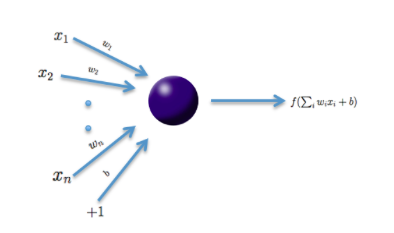
\includegraphics[scale = 0.9,angle = 0]{figure/neuralNet.png}
  \caption[Neural Network]{\normalsize{Neural Network}}
  \label{fig:Hyarn6}
  \end{figure}
  
  \begin{figure}[htbp]
  \centering
  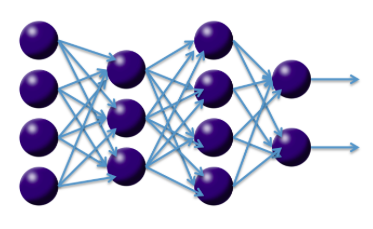
\includegraphics[scale = 0.5,angle = 0]{figure/neuralHid.png}
  \caption[Hidden Layers]{\normalsize{Hidden Layers}}
  \label{fig:Hyarn7}
  \end{figure}
  
  Overall H2O's deep learning functionalities include specification of
  regularization options, learning rate, annealing, hyperparameter
  optimization and model selection through grid and random search.
  Additionally H2O facilitates automatic processing for categorical and
  numerical data along with automatic imputation of missing values and
  ensurance of fast convergence.
  
  H2O was used to perform deep learning to predict departure delay greater
  than 90 minutes. The response variable was a continuous predictor
  capturing extent of departure delay in minutes. This dataset differed
  from the dataset used to perform logistic regression since the latter
  contained a binary predictor to predict whether or not departure delay
  greater than 30 minutes occurred. In the deep learning scenario, the
  explanatory variables of interest included year, month, arrival delay,
  carrier, distance, hour, week, weekend and season.
  
  \clearpage 
  
  \section{Data Partitioning}\label{data-partitioning-2}
  
  Before data preparation and model building, connection was established
  to the YARN client. Following connection, data sample of 200000 was
  obtained given that this data size was easily transferable to the Spark
  environment. Since hyperparameter optimization was performed in the deep
  learning algorithm, a validation data set was used along with the test
  set for additional verification. Data split was split with 60/20/20
  split consisting of 60\% training, 20\% validation and 20\% test set.
  
  \begin{Shaded}
  \begin{Highlighting}[]
  \KeywordTok{options}\NormalTok{(}\DataTypeTok{rsparkling.sparklingwater.version =} \StringTok{"1.6.8"}\NormalTok{)}
  \NormalTok{sc <-}\StringTok{ }\KeywordTok{spark_connect}\NormalTok{(}\DataTypeTok{master =} \StringTok{"yarn-client"}\NormalTok{)}
  
  \KeywordTok{set.seed}\NormalTok{(}\DecValTok{12}\NormalTok{)}
  \NormalTok{thousand <-}\StringTok{ }\NormalTok{FullDat[}\KeywordTok{sample}\NormalTok{(}\KeywordTok{nrow}\NormalTok{(FullDat), }\DecValTok{200000}\NormalTok{, }\DataTypeTok{replace =} \OtherTok{FALSE}\NormalTok{, }
                             \DataTypeTok{prob =} \OtherTok{NULL}\NormalTok{),]}
  \NormalTok{mtcars_tbl <-}\StringTok{ }\KeywordTok{copy_to}\NormalTok{(sc, thousand, }\StringTok{"mtcars"}\NormalTok{, }\DataTypeTok{overwrite =} \OtherTok{TRUE}\NormalTok{) }
  
  \NormalTok{partitions <-}\StringTok{ }\NormalTok{mtcars_tbl %>%}
  \StringTok{  }\KeywordTok{sdf_partition}\NormalTok{(}\DataTypeTok{training =} \FloatTok{0.6}\NormalTok{, }\DataTypeTok{validation =} \FloatTok{0.20}\NormalTok{, }\DataTypeTok{test =} \FloatTok{0.20}\NormalTok{, }
                  \DataTypeTok{seed =} \DecValTok{1099}\NormalTok{)}
  \end{Highlighting}
  \end{Shaded}
  
  \clearpage 
  
  \section{Model Building}\label{model-building}
  
  Following data partitioning, h2o.deeplearning function was used to
  predict departure delay over 90 minutes as a function of year, month,
  arrival delay, carrier, distance, hour, week, weekend and season. The
  h2o.deeplearning function includes specification of the explanatory (x)
  and response predictors (y). In addition, h2o.deeplearning paramaters
  include activation function specification (Tanh, TanhWithDropout,
  Rectifier, RectifierWithDropout, Maxout, MaxoutWithDropout, see
  \autoref{fig:Hyarn77} (Candel et al., 2015)), training and
  validation\_frame delineation along with fine-tuning parameters like
  maximum model iterations, regularization parameters like l1 and l2,
  non-negative shrinkage parameter lambda and cross validation parameter
  (nfolds) specifying number of folds and model iterations. A random seed
  can also be specified though this is only reproducible with algorithms
  running on a single thread. Additionally h2o.deeplearning model provides
  the ability to stop the model learning early if no apparent changes in
  the loss function are observed.
  
  \begin{figure}[htbp]
  \centering
  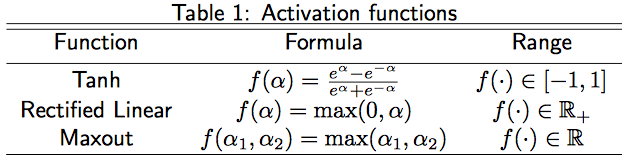
\includegraphics[scale = 0.5,angle = 0]{figure/activationFunc.png}
  \caption[Activation Function]{\normalsize{Activation Function}}
  \label{fig:Hyarn77}
  \end{figure}
  
  A simple model shown below was constructed to predict departure delay
  over 90 minutes as a function of the explantory variables. Epoch of one
  was used indicating a single data iteration. In addition, 5 folds cross
  validation was used. Tanh activation layer was used since it is more
  adept at exponentially rising functions and consequently better at
  containing regularization.
  
  \begin{Shaded}
  \begin{Highlighting}[]
  \NormalTok{myX =}\StringTok{ }\KeywordTok{setdiff}\NormalTok{(}\KeywordTok{colnames}\NormalTok{(training), (}\StringTok{"dep_delay"}\NormalTok{))}
  \NormalTok{deepmod <-}\StringTok{ }\KeywordTok{h2o.deeplearning}\NormalTok{(}
    \DataTypeTok{y=}\StringTok{"dep_delay"}\NormalTok{,}
    \DataTypeTok{x=}\NormalTok{myX,}
    \DataTypeTok{activation=}\StringTok{"Tanh"}\NormalTok{,  }
    \DataTypeTok{training_frame=}\NormalTok{training, }
    \DataTypeTok{validation_frame=}\NormalTok{validation,}
    \DataTypeTok{epochs=}\DecValTok{1}\NormalTok{,}
    \DataTypeTok{variable_importances=}\NormalTok{T,   }
    \DataTypeTok{nfolds =} \DecValTok{5}\NormalTok{,}
    \DataTypeTok{keep_cross_validation_predictions=}\NormalTok{T}
  \NormalTok{)}
  \end{Highlighting}
  \end{Shaded}
  
  A variable importance plot can be used to view the most important
  predictors produced by deepmod. In this case, a plot of the top 20
  predictors was produced. As \autoref{fig:Hyarn81} shows, arrival delay
  appeared to be most important at predicting departure delay greater than
  90 minutes. Following arrival delay, day status (weekday or weekend) was
  the next important predictor. Continental Airlines (CO), Comair, Inc.
  (OH) and 9 Air Co Ltd were most important carriers in predicting
  departure delay. Additionally hour 14 (2 pm) appeared to be important in
  predicting departure delay greater than 90 minutes.
  
  \begin{Shaded}
  \begin{Highlighting}[]
  \KeywordTok{h2o.varimp_plot}\NormalTok{(deepmod, }\DataTypeTok{num_of_features =} \DecValTok{20}\NormalTok{)}
  \end{Highlighting}
  \end{Shaded}
  
  \begin{figure}[htbp]
  \centering
  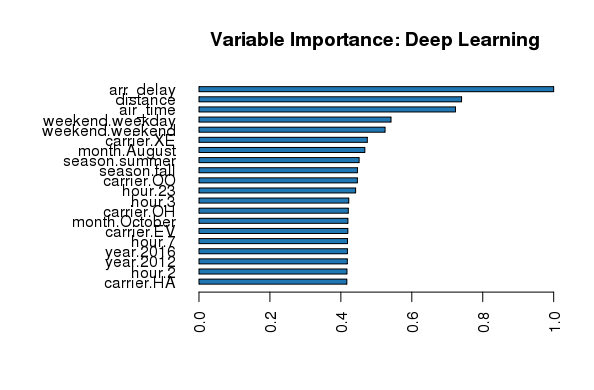
\includegraphics[scale = 1,angle = 0]{figure/VarImportDeep-3.png}
  \caption[Deep Learning Variable Importance]{\normalsize{Deep Learning Variable Importance}}
  \label{fig:Hyarn81}
  \end{figure}
  
  \clearpage 
  
  \section{Model Assessment}\label{model-assessment-2}
  
  Deep learning model performance was assessed. Since the response
  predictor is continuous, mean squared error (MSE) was used as an error
  metric.
  
  As shown by \autoref{fig:Hyarn9}, MSE on training data was 459.14 while
  MSE on validation data was 472.58. In comparison, MSE on test data was
  491.59. Since MSE for the validation and test data is higher than MSE on
  training data, this was an indication of good fit. Overfitting did not
  appear t o be extremely visible since the difference between the MSE of
  the training, validation and test set did not appear to be too visible.
  
  \begin{Shaded}
  \begin{Highlighting}[]
  \NormalTok{deepmod@parameters  }
  \KeywordTok{h2o.performance}\NormalTok{(deepmod, }\DataTypeTok{train =} \OtherTok{TRUE}\NormalTok{)  }
  \KeywordTok{h2o.performance}\NormalTok{(deepmod, }\DataTypeTok{valid =} \OtherTok{TRUE}\NormalTok{)  }
  \KeywordTok{h2o.performance}\NormalTok{(deepmod, }\DataTypeTok{newdata =} \NormalTok{test)}
  \end{Highlighting}
  \end{Shaded}
  
  \begin{figure}[htbp]
  \centering
  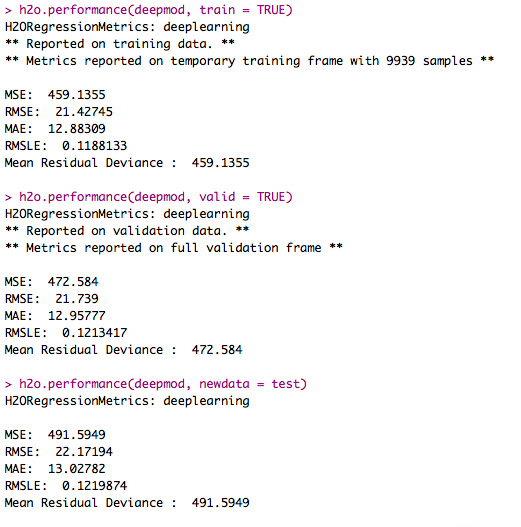
\includegraphics[scale = 0.7,angle = 0]{figure/deepModml.png}
  \caption[Deep Learning Model Performance]{\normalsize{Deep Learning Model Performance}}
  \label{fig:Hyarn9}
  \end{figure}
  
  \clearpage 
  
  \section{Saving Model}\label{saving-model}
  
  Once the model was constructed, it was saved using the h2o.saveModel
  command as shown below with the path specification.
  
  \begin{Shaded}
  \begin{Highlighting}[]
  \NormalTok{DeepModel <-}\StringTok{ }\KeywordTok{h2o.saveModel}\NormalTok{(m1, }\DataTypeTok{path =} \StringTok{"/home/ajavaid17"}\NormalTok{, }\DataTypeTok{force =} \OtherTok{FALSE}\NormalTok{) }
  \end{Highlighting}
  \end{Shaded}
  
  Model can be loaded with the h2o.loadModel command with the specified
  path as an argument.
  
  \begin{Shaded}
  \begin{Highlighting}[]
  \NormalTok{ld <-}\StringTok{ }\KeywordTok{h2o.loadModel}\NormalTok{(}\DataTypeTok{path =}\StringTok{"/home/ajavaid17/}
  \StringTok{                    DeepLearning_model_R_1487567612904_2"}\NormalTok{)}
  \end{Highlighting}
  \end{Shaded}
  
  \section{Grid Search Model}\label{grid-search-model}
  
  H2O provides grid search functionality which allows the user to
  experiment with different hyperparameter combinations. All possible
  combinations of the hyperparameters are tested. In the model below, 2
  different activation functions, 2 hidden layers, 2 input\_dropout\_ratio
  and 3 rate parameters were tested resulting in 24 models. Tanh and
  TanhWithDropout parameters were used since they better regularize for
  exponential functions. The hidden variable specifies the hidden layer
  sizes. The rate parameter specifies the learning rate where a higher
  rate produces less model stability and a lower rate produces slower
  model convergence. The rate\_annealing parameter attempts to adjust
  learning rate.
  
  \begin{Shaded}
  \begin{Highlighting}[]
  \NormalTok{hyper_params <-}\StringTok{ }\KeywordTok{list}\NormalTok{(}
    \DataTypeTok{activation=}\KeywordTok{c}\NormalTok{(}\StringTok{"Tanh"}\NormalTok{, }\StringTok{"TanhWithDropout"}\NormalTok{),}
    \DataTypeTok{hidden=}\KeywordTok{list}\NormalTok{(}\KeywordTok{c}\NormalTok{(}\DecValTok{20}\NormalTok{,}\DecValTok{20}\NormalTok{),}\KeywordTok{c}\NormalTok{(}\DecValTok{40}\NormalTok{,}\DecValTok{40}\NormalTok{)),}
    \DataTypeTok{input_dropout_ratio=}\KeywordTok{c}\NormalTok{(}\DecValTok{0}\NormalTok{,}\FloatTok{0.05}\NormalTok{),}
    \DataTypeTok{rate=}\KeywordTok{c}\NormalTok{(}\FloatTok{0.01}\NormalTok{,}\FloatTok{0.02}\NormalTok{,}\FloatTok{0.03}\NormalTok{)}
  \NormalTok{)}
  \end{Highlighting}
  \end{Shaded}
  
  After setting up the hyperparameters, h2o.grid functionality was used to
  iterate over models. In order to expedite the model building process,
  stopping metrics were specified so the h2o.grid functionality stops when
  the MSE does not improve by greater than or equal to 2\%
  (stopping\_tolerance) for 2 events (stopping\_rounds). In addition to
  the hyperparameters specified, epoch of 10 was chosen. Momentum was
  specified to reduce the chance of the algorithm halting at a local
  minima. Theoretically, momentum specification reduces terrrain
  irregularities thus preventing algorithm to stop at the minima
  (Sutskever, Martens, Dahl, \& Hinton, 2013). The l1 and l2
  regularization parameters attempt to prevent overfitting while the
  max\_w2 sets the constraint for squared sum of incoming weights per
  unit.
  
  \begin{Shaded}
  \begin{Highlighting}[]
  \NormalTok{grid <-}\StringTok{ }\KeywordTok{h2o.grid}\NormalTok{(}
    \DataTypeTok{algorithm=}\StringTok{"deeplearning"}\NormalTok{,}
    \DataTypeTok{grid_id=}\StringTok{"gridDeep"}\NormalTok{, }
    \DataTypeTok{training_frame=}\NormalTok{training,}
    \DataTypeTok{validation_frame=}\NormalTok{validation,}
    \DataTypeTok{y=}\StringTok{"dep_delay"}\NormalTok{,}
    \DataTypeTok{x=}\NormalTok{myX,}
    \DataTypeTok{epochs=}\DecValTok{10}\NormalTok{,}
    \DataTypeTok{stopping_metric=}\StringTok{"MSE"}\NormalTok{,}
    \DataTypeTok{stopping_tolerance=}\FloatTok{2e-2}\NormalTok{,        }
    \DataTypeTok{stopping_rounds=}\DecValTok{2}\NormalTok{, }
    \DataTypeTok{score_duty_cycle=}\FloatTok{0.025}\NormalTok{,         }
    \DataTypeTok{adaptive_rate=}\NormalTok{T,                }
    \DataTypeTok{momentum_start=}\FloatTok{0.5}\NormalTok{,             }
    \DataTypeTok{momentum_stable=}\FloatTok{0.9}\NormalTok{, }
    \DataTypeTok{momentum_ramp=}\FloatTok{1e7}\NormalTok{,}
    \DataTypeTok{variable_importances=}\NormalTok{T,}
    \DataTypeTok{l1=}\FloatTok{1e-5}\NormalTok{,                         }
    \DataTypeTok{l2=}\FloatTok{1e-5}\NormalTok{,}
    \DataTypeTok{max_w2=}\DecValTok{10}\NormalTok{, }
    \DataTypeTok{hyper_params=}\NormalTok{hyper_params}
  \NormalTok{)}
  \end{Highlighting}
  \end{Shaded}
  
  For loop can be used to iterate over all 24 models to output the MSE.
  Direct indexing in the grid object can be used to retrieve the optimal
  model along with associated parameters. The gridDeep grid search
  resulted in an optimal model with parameters including the Tanh
  activation layer, hidden layer of (40,40), input\_dropout\_ratio of 0
  and rate of 0.01 as depicted by \autoref{fig:Hyarn11}.
  
  \begin{Shaded}
  \begin{Highlighting}[]
  \NormalTok{for (model_id in grid@model_ids) \{}
    \NormalTok{model <-}\StringTok{ }\KeywordTok{h2o.getModel}\NormalTok{(model_id)}
    \NormalTok{mse <-}\StringTok{ }\KeywordTok{h2o.mse}\NormalTok{(model, }\DataTypeTok{valid =} \OtherTok{TRUE}\NormalTok{) }
    \KeywordTok{sprintf}\NormalTok{(}\StringTok{"Validation set MSE: %f"}\NormalTok{, mse)}
  \NormalTok{\}}
  
  \CommentTok{#Retrieve optimal model by MSE}
  \NormalTok{grid@summary_table[}\DecValTok{1}\NormalTok{,] }
  \NormalTok{optimal <-}\StringTok{ }\KeywordTok{h2o.getModel}\NormalTok{(grid@model_ids[[}\DecValTok{1}\NormalTok{]]) }
  
  \NormalTok{optimal@allparameters }\CommentTok{#print all parameters of best model }
  \KeywordTok{h2o.performance}\NormalTok{(optimal, }\DataTypeTok{train =} \OtherTok{TRUE}\NormalTok{) }\CommentTok{#retrieve training MSE}
  \KeywordTok{h2o.performance}\NormalTok{(optimal, }\DataTypeTok{valid =} \OtherTok{TRUE}\NormalTok{) }\CommentTok{#retrieve validation MSE}
  \KeywordTok{h2o.performance}\NormalTok{(optimal, }\DataTypeTok{newdata =} \NormalTok{test) }\CommentTok{#retrieve test MSE }
  \end{Highlighting}
  \end{Shaded}
  
  \begin{figure}[htbp]
  \centering
  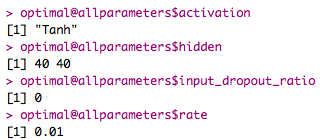
\includegraphics[scale = 0.7,angle = 0]{figure/optimalParam.png}
  \caption[Grid Model Parameters]{\normalsize{Grid Model Parameters}}
  \label{fig:Hyarn11}
  \end{figure}
  
  As shown by \autoref{fig:Hyarn122}, MSE on the optimal model for the
  training data was 328.50 whereas MSE for the validation data was 379.50
  and 393.25 for the test data. The validation and test errors were higher
  than training signaling towards a good model fit, with some reservations
  for overfitting. Grid search model performs better than a simple deep
  model since the MSE for the grid search model are lower than the MSE for
  deepmod (training MSE of 459.14, validation MSE of 472.58 and test MSE
  of 491.59).
  
  \begin{figure}[htbp]
  \centering
  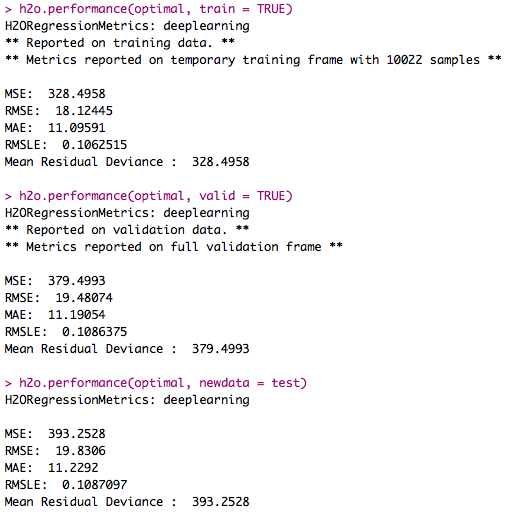
\includegraphics[scale = 0.8,angle = 0]{figure/DeepGridPerform.png}
  \caption[Grid Model Performance]{\normalsize{Grid Model Performance}}
  \label{fig:Hyarn122}
  \end{figure}
  
  Variable importance plot can be used to view the most important
  predictors. As \autoref{fig:Hyarn89} shows, arrival delay appears to be
  most important in predicting departure delay greater than 90 minutes.
  Following arrival delay, distance and air time appear to be next
  important. JetSuite Air (XE) appears to be the most important carrier in
  predicting departure delay greater than 90 minutes. Season summer and
  month August additionally appear to be important in predicting departure
  delay greater than 90 minutes.
  
  \begin{Shaded}
  \begin{Highlighting}[]
  \KeywordTok{h2o.varimp_plot}\NormalTok{(optimal, }\DataTypeTok{num_of_features =} \DecValTok{20}\NormalTok{)}
  \end{Highlighting}
  \end{Shaded}
  
  \begin{figure}[htbp]
  \centering
  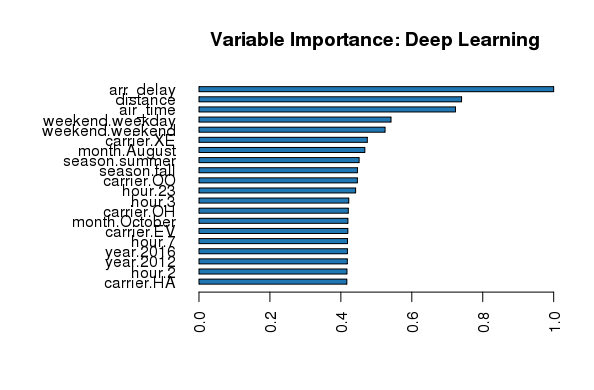
\includegraphics[scale = 1,angle = 0]{figure/VarImportDeep-3.png}
  \caption[Grid Search Variable Importance]{\normalsize{Grid Search Variable Importance}}
  \label{fig:Hyarn89}
  \end{figure}
  
  \clearpage 
  
  \section{Random Grid Search Model}\label{random-grid-search-model}
  
  In comparison to grid search which iterated over combinations
  exhaustively and sequentially, random grid search model can be used to
  accelerate the process of hyperparameter selection. This is particularly
  useful in situations where the user wants to consider a large number of
  hyperparameters. Random grid search proceeds to randomly search the user
  specified space using an established search criteria. Since random grid
  search model was used, additional hyperparameters were assessed for
  analysis. As shown below, Tanh and TanhWithDropout functions were
  tested. The hidden layer additionally included (30,30,30), (50,50) and
  (70,70). Rate 0.03 was also tested along with 0.0 and 0.02. In addition,
  different combinations of regularization parameters (l1 and l2) were
  tested.
  
  \begin{Shaded}
  \begin{Highlighting}[]
  \NormalTok{hyper_params <-}\StringTok{ }\KeywordTok{list}\NormalTok{(}
    \DataTypeTok{activation=}\KeywordTok{c}\NormalTok{(}\StringTok{"Tanh"}\NormalTok{,}\StringTok{"TanhWithDropout"}\NormalTok{),}
    \DataTypeTok{hidden=}\KeywordTok{list}\NormalTok{(}\KeywordTok{c}\NormalTok{(}\DecValTok{20}\NormalTok{,}\DecValTok{20}\NormalTok{),}\KeywordTok{c}\NormalTok{(}\DecValTok{30}\NormalTok{,}\DecValTok{30}\NormalTok{,}\DecValTok{30}\NormalTok{),}\KeywordTok{c}\NormalTok{(}\DecValTok{40}\NormalTok{,}\DecValTok{40}\NormalTok{,}\DecValTok{40}\NormalTok{),}\KeywordTok{c}\NormalTok{(}\DecValTok{50}\NormalTok{,}\DecValTok{50}\NormalTok{),}\KeywordTok{c}\NormalTok{(}\DecValTok{70}\NormalTok{,}\DecValTok{70}\NormalTok{)),}
    \DataTypeTok{input_dropout_ratio=}\KeywordTok{c}\NormalTok{(}\DecValTok{0}\NormalTok{,}\FloatTok{0.05}\NormalTok{),}
    \DataTypeTok{rate=}\KeywordTok{c}\NormalTok{(}\FloatTok{0.01}\NormalTok{,}\FloatTok{0.02}\NormalTok{,}\FloatTok{0.03}\NormalTok{),}
    \DataTypeTok{l1=}\KeywordTok{seq}\NormalTok{(}\DecValTok{0}\NormalTok{,}\FloatTok{1e-4}\NormalTok{,}\FloatTok{1e-6}\NormalTok{),}
    \DataTypeTok{l2=}\KeywordTok{seq}\NormalTok{(}\DecValTok{0}\NormalTok{,}\FloatTok{1e-4}\NormalTok{,}\FloatTok{1e-6}\NormalTok{)}
  \NormalTok{)}
  \end{Highlighting}
  \end{Shaded}
  
  With the hyperparameters specified, next step included defining the
  search criteria. As the criteria below shows, the algorithm was defined
  to stop when the top 5 models were within 2\% of each other. Max model
  running time was 600 seconds (10 minutes). In addition to the max
  running time, number of max\_models can also be specified.
  
  \begin{Shaded}
  \begin{Highlighting}[]
  \NormalTok{search_criteria =}\StringTok{ }\KeywordTok{list}\NormalTok{(}\DataTypeTok{strategy =} \StringTok{"RandomDiscrete"}\NormalTok{, }
                         \DataTypeTok{max_runtime_secs =} \DecValTok{600}\NormalTok{, }\DataTypeTok{max_models =} \DecValTok{100}\NormalTok{, }
                         \DataTypeTok{seed=}\DecValTok{22}\NormalTok{, }\DataTypeTok{stopping_rounds=}\DecValTok{5}\NormalTok{, }
                         \DataTypeTok{stopping_tolerance=}\FloatTok{2e-2}\NormalTok{)}
  \end{Highlighting}
  \end{Shaded}
  
  Following delineation of the search criteria, the h2o.grid function can
  be used to specify additional fixed parameters. These include definition
  of epochs of 10, max\_w2 of 10, score\_validation\_samples of 10000 and
  score\_duty\_cycles of 0.025. The score\_validation\_samples specify the
  number of validation set samples for scoring while the
  score\_duty\_cycles specifies the maximum duty cycle fraction for
  scoring. The same stopping parameters as the grid search model were
  used. The algorithm was thus indicated to stop when the MSE does not
  improve by at least 2\% for 2 scoring events.
  
  \begin{Shaded}
  \begin{Highlighting}[]
  \NormalTok{random_grid <-}\StringTok{ }\KeywordTok{h2o.grid}\NormalTok{(}
    \DataTypeTok{algorithm=}\StringTok{"deeplearning"}\NormalTok{,}
    \DataTypeTok{grid_id =} \StringTok{"Gridrandom"}\NormalTok{,}
    \DataTypeTok{training_frame=}\NormalTok{training,}
    \DataTypeTok{validation_frame=}\NormalTok{validation, }
    \DataTypeTok{x=}\NormalTok{myX, }
    \DataTypeTok{y=}\StringTok{"dep_delay"}\NormalTok{,}
    \DataTypeTok{epochs=}\DecValTok{10}\NormalTok{,}
    \DataTypeTok{stopping_metric=}\StringTok{"MSE"}\NormalTok{,}
    \DataTypeTok{stopping_tolerance=}\FloatTok{2e-2}\NormalTok{,        }
    \DataTypeTok{stopping_rounds=}\DecValTok{2}\NormalTok{,}
    \DataTypeTok{score_validation_samples=}\DecValTok{10000}\NormalTok{, }
    \DataTypeTok{score_duty_cycle=}\FloatTok{0.025}\NormalTok{,         }
    \DataTypeTok{max_w2=}\DecValTok{10}\NormalTok{,                      }
    \DataTypeTok{hyper_params =} \NormalTok{hyper_params,}
    \DataTypeTok{search_criteria =} \NormalTok{search_criteria}
  \NormalTok{)}
  \end{Highlighting}
  \end{Shaded}
  
  The validation set MSE for all the random search models can be printed
  with a for loop. Additionally, the best model and its associated
  parameters can be viewed. As shown by \autoref{fig:Hyarn111}, optimal
  model generated by random grid search has an activation function of
  Tanh, hidden layer of (30,30,30), input\_dropout\_ratio of 0, rate of
  0.02, l1 of 2.3e-05 and l2 of 7.6e-05.
  
  \begin{Shaded}
  \begin{Highlighting}[]
  \NormalTok{for (model_id in grid@model_ids) \{}
    \NormalTok{model <-}\StringTok{ }\KeywordTok{h2o.getModel}\NormalTok{(model_id)}
    \NormalTok{mse <-}\StringTok{ }\KeywordTok{h2o.mse}\NormalTok{(model, }\DataTypeTok{valid =} \OtherTok{TRUE}\NormalTok{) }
    \KeywordTok{sprintf}\NormalTok{(}\StringTok{"Validation set MSE: %f"}\NormalTok{, mse)}
  \NormalTok{\}}
  
  \CommentTok{#Retrieve optimal model by MSE}
  \NormalTok{grid@summary_table[}\DecValTok{1}\NormalTok{,] }
  \NormalTok{optimal <-}\StringTok{ }\KeywordTok{h2o.getModel}\NormalTok{(grid@model_ids[[}\DecValTok{1}\NormalTok{]]) }
  
  \NormalTok{optimal@allparameters }\CommentTok{#print all parameters of best model }
  \KeywordTok{h2o.performance}\NormalTok{(optimal, }\DataTypeTok{train =} \OtherTok{TRUE}\NormalTok{) }\CommentTok{#retrieve training MSE}
  \KeywordTok{h2o.performance}\NormalTok{(optimal, }\DataTypeTok{valid =} \OtherTok{TRUE}\NormalTok{) }\CommentTok{#retrieve validation MSE}
  \KeywordTok{h2o.performance}\NormalTok{(optimal, }\DataTypeTok{newdata =} \NormalTok{test) }\CommentTok{#retrieve test MSE }
  \end{Highlighting}
  \end{Shaded}
  
  \begin{figure}[htbp]
  \centering
  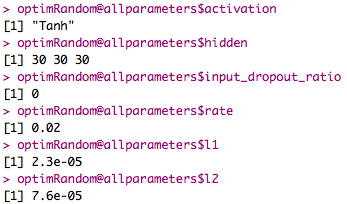
\includegraphics[scale = 0.7,angle = 0]{figure/optimRandomParam.png}
  \caption[Random Grid Model Parameters]{\normalsize{Random Grid Model Parameters}}
  \label{fig:Hyarn111}
  \end{figure}
  
  As \autoref{fig:Hyarn124} indicates, the MSE on the optimal random model
  for the training data was 306.25 whereas MSE for the validation set was
  309.64 and 412.57 for the test set. The training and validation error
  are lower than those yielded by the grid search model (328.50 for
  training and 379.50 for validation) while the test error for the random
  search model is higher than the test error for the grid search model
  (393.25 for grid search test model). Since the random search test error
  is much higher than the training MSE, there may be some presence of
  overfitting. The errors for the random search model are lower than the
  initial deep learning model deepmod (training MSE of 374.39, validation
  MSE of 430.06 and test MSE of 423.41).
  
  \begin{figure}[htbp]
  \centering
  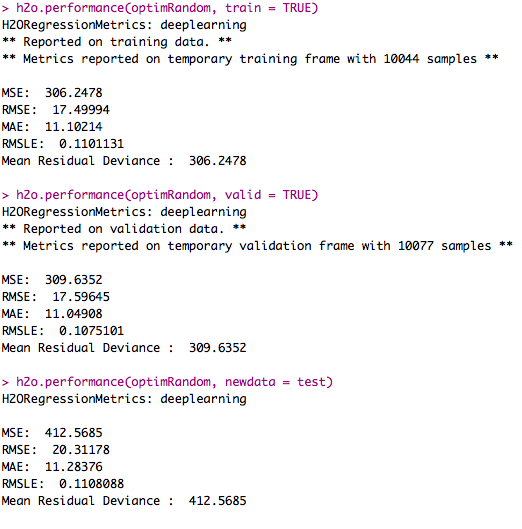
\includegraphics[scale = 0.8,angle = 0]{figure/DeepGridPerformRand.png}
  \caption[Random Grid Performance]{\normalsize{Random Grid Performance}}
  \label{fig:Hyarn124}
  \end{figure}
  
  Variable importance plot can be used to view the most important
  predictors. In this case, a plot of the top 20 predictors was produced.
  As \autoref{fig:Hyarn139} shows, arrival delay appears to be the most
  important predictor in predicting departure delay greater than 90
  minutes. Following arrival delay, air time and distance appear to be the
  next important predictors. Additionally hour 4 (4 am), hour 5 (5 am),
  hour 0 (12 am) and weekend appear to be the next important predictors.
  Spirit appears to be the most important carrier in predicting departure
  delay greater than 90 minutes.
  
  \begin{Shaded}
  \begin{Highlighting}[]
  \KeywordTok{h2o.varimp_plot}\NormalTok{(optimal, }\DataTypeTok{num_of_features =} \DecValTok{20}\NormalTok{)}
  \end{Highlighting}
  \end{Shaded}
  
  \begin{figure}[htbp]
  \centering
  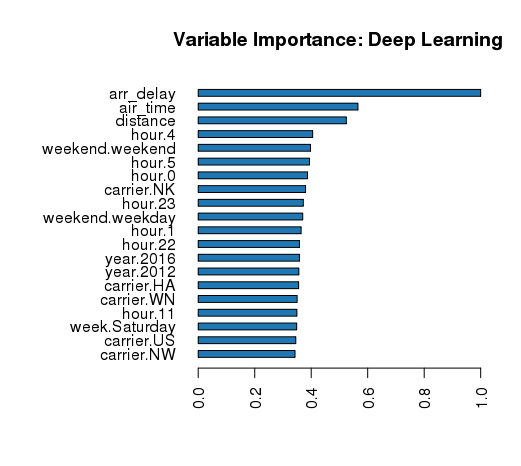
\includegraphics[scale = 1,angle = 0]{figure/VarImportRand-2.png}
  \caption[Random Grid Variable Importance]{\normalsize{Random Grid Variable Importance}}
  \label{fig:Hyarn139}
  \end{figure}
  
  \clearpage 
  
  \section{Checkpoint Model}\label{checkpoint-model}
  
  Checkpoint functionality can be used in H2O to continue iterations from
  a previously built model. Checkpoint option allows specification of a
  previously built model key. The new model is then built as a
  continuation of the old model. If the model key is not supplied, then a
  new model is built instead. In the checkpoint model, the value of the
  parameters must be greater than their value set in the previous model.
  Parameters like activation function, max\_categorical\_features,
  momentum\_ramp, momentum\_stable, momentum\_start and nfolds cannot be
  modified. A full list of all the parameters that cannot be modified can
  be found at
  (\url{http://docs.h2o.ai/h2o/latest-stable/h2o-docs/data-science/algo-params/checkpoint.html})\footnote{(``Checkpoint,''
    n.d.)}.
  
  Since the test MSE (412.57) produced by the random search model was much
  higher than the errors on the training (306.25) and validation set
  (309.64), higher l1 and l2 parameters were used to produce better
  performance on the test set. Additionally epochs of 20 were used. These
  additional parameters were specified from the initial basis of the
  optimal random grid search model, specified below in the checkpoint
  specification as Gridrandom6\_model\_6. Same activation (Tanh), hidden
  layer (30,30,30) and rate (0.02) were used since these parameters can't
  be altered in the checkpoint model.
  
  \begin{Shaded}
  \begin{Highlighting}[]
  \NormalTok{max_epochs <-}\StringTok{ }\DecValTok{20} 
  \NormalTok{checkpoint <-}\StringTok{ }\KeywordTok{h2o.deeplearning}\NormalTok{(}
    \DataTypeTok{model_id=}\StringTok{"GridModRandom_continued2"}\NormalTok{, }
    \DataTypeTok{activation=}\StringTok{"Tanh"}\NormalTok{,}
    \DataTypeTok{checkpoint=}\StringTok{"Gridrandom6_model_6"}\NormalTok{, }
    \DataTypeTok{training_frame=}\NormalTok{training, }
    \DataTypeTok{validation_frame=}\NormalTok{validation, }
    \DataTypeTok{y=}\StringTok{"dep_delay"}\NormalTok{,}
    \DataTypeTok{x=}\NormalTok{myX, }
    \DataTypeTok{hidden=}\KeywordTok{c}\NormalTok{(}\DecValTok{30}\NormalTok{,}\DecValTok{30}\NormalTok{,}\DecValTok{30}\NormalTok{),          }
    \DataTypeTok{epochs=}\NormalTok{max_epochs,              }
    \DataTypeTok{stopping_metric=}\StringTok{"MSE"}\NormalTok{,     }
    \DataTypeTok{stopping_tolerance=}\FloatTok{2e-2}\NormalTok{,       }
    \DataTypeTok{stopping_rounds=}\DecValTok{2}\NormalTok{,}
    \DataTypeTok{score_duty_cycle=}\FloatTok{0.025}\NormalTok{,         }
    \DataTypeTok{adaptive_rate=}\NormalTok{T,                }
    \DataTypeTok{l1=}\FloatTok{1e-4}\NormalTok{,                        }
    \DataTypeTok{l2=}\FloatTok{1e-4}\NormalTok{,}
    \DataTypeTok{max_w2=}\DecValTok{10}\NormalTok{,}
    \DataTypeTok{rate =} \FloatTok{0.02}\NormalTok{,}
    \DataTypeTok{variable_importances=}\NormalTok{T}
  \NormalTok{) }
  \end{Highlighting}
  \end{Shaded}
  
  As shown by \autoref{fig:Hyarn143}, MSE on the training data was 356.75,
  388.46 for validation and 399.96 for the test data. The test MSE is much
  closer to the validation set whereas MSE previously on the random grid
  search test data was 412.57. Since the test MSE is closer to the
  training and validation set's MSE, this reduces chance of overfitting.
  
  \begin{figure}[htbp]
  \centering
  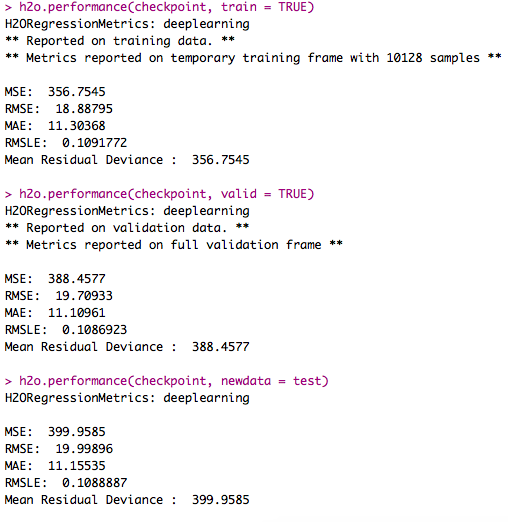
\includegraphics[scale = 0.7,angle = 0]{figure/DeepGridCheckpoint.png}
  \caption[Checkpoint Performance]{\normalsize{Checkpoint Performance}}
  \label{fig:Hyarn143}
  \end{figure}
  
  According to the variable importance chart shown by
  \autoref{fig:Hyarn17}, arrival delay appears to be most important in
  predicting departure delay greater than 90 minutes. Hour 4 (4 am), air
  time, hour 0 (12 am) and hour 5 (5 am) appear to be next important.
  Additionally Spirit appears to be an important carrier in predicting
  departure delay greater than 90 minutes.
  
  \begin{figure}[htbp]
  \centering
  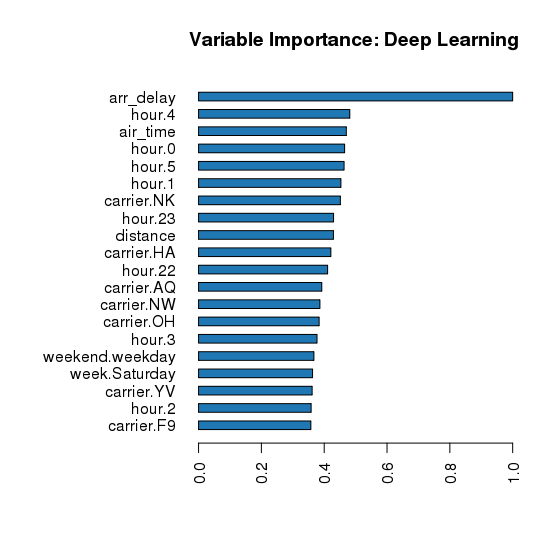
\includegraphics[scale = 0.9,angle = 0]{figure/VarImportCheckpoint.png}
  \caption[Checkpoint Variable Importance]{\normalsize{Checkpoint Variable Importance}}
  \label{fig:Hyarn17}
  \end{figure}
  
  \clearpage 
  
  \section{Conclusions}\label{conclusions}
  
  This chapter discussed deep learning models including concepts like
  setting up hyperparameters for deep learning models through the grid
  search and random search methods. In addition, the checkpoint model
  functionality was discussed.
  
  Overall, arrival delay appears to be most important in predicting
  departure delay greater than 90 minutes which indicates that airlines
  experiencing arrival delay appear to have a higher likelihood of
  experiencing departure delays. Additional important predictors include
  amount of distance covered as well as the amount of air time. Early
  morning hours between 12-5 am and weekend also appear to be important
  predictors of departure delay greater than 90 minutes, a trend that was
  also observed in the shiny app exploratory analysis.
  
  In regards to model performance, the grid search model improved upon the
  original simple deep learning model. The random search model produced
  similar and in some regards better results than the grid search model
  (lower MSE on training and validation sets). Checkpoint model improved
  upon the random search model by reducing the test set MSE, thus lowering
  incidence of overfitting.
  
  \chapter*{Conclusion}\label{conclusion-2}
  \addcontentsline{toc}{chapter}{Conclusion}
  
  This project involved navigation of both the R and Hadoop servers. The
  h2o and rsparkling packages were explored amongst others. Shiny
  application was used for initial data and network exploration. H2O
  platform was used to perform logistic modeling and deep learning to
  predict the occurrence of departure delay greater than 30 minutes
  (binary outcome) and extent of departure delay greater than 90 minutes
  (continuous outcome). Additionally weather was incorporated for
  logistical analysis. Web scraping was also performed to extract full
  airport and state names. Conceptually, this project explored topics like
  big data infrastructure of technologies like Hadoop and Apache Spark,
  neural networks and feed-forward learning and machine learning
  hyperparameter optimization through grid and random search models.
  
  \section{Limitations}\label{limitations}
  
  One limitation of this study was that only sample of 200000 was copied
  in the Spark environment although the original dataset had about a
  million observations. Capacity of Spark can be improved to handle
  additional data. Parallel computing through the parallel package can
  also be pursued to explore how the data can be split in smaller datasets
  with computations performed on each in a separate Spark connection and
  later aggregated/merged. Additionally my model shows an increase in
  departure delay overtime from 2008 to 2016 which seems counterintuitive.
  It may be worthwhile to examine this finding further and assess whether
  there are potential confounders clouding the result.
  
  \section{Future Work}\label{future-work}
  
  Future extensions of this project can include building data pipelines to
  dynamically collect weather data for the associated flights and store
  the data in a Hadoop database. Additionally data containing security
  alerts can be used to gauge whether flight delays have been associated
  with increased alerts. Data on computer glitches and technical
  abnormalities as related to departure delay would also be insightful. In
  the future, data on plane manufacturer can be obtained to gauge whether
  or not the extent of departure delay experienced by a plane is
  associated with its manufactured date. In the future, tracing the
  departure delay experienced by a flight can be analyzed to observe
  whether or not the extent of delay is related to delay experienced by
  the connecting flight. Additionally other machine learning models can be
  explored besides feed-forward neural network employed in deep learning.
  These methods include SVMs, gradient boosters and ensemble modeling.
  
  \appendix
  
  \chapter{The First Appendix}\label{the-first-appendix}
  
  There were no hidden code chunks in the paper. See the second appendix
  for accessory code.
  
  \chapter{The Second Appendix, for
  Fun}\label{the-second-appendix-for-fun}
  
  \subsubsection{Creation of the FullDat dataset (flights data from 2008
  to
  2016)}\label{creation-of-the-fulldat-dataset-flights-data-from-2008-to-2016}
  
  \begin{Shaded}
  \begin{Highlighting}[]
  \KeywordTok{library}\NormalTok{(sparklyr)}
  \KeywordTok{library}\NormalTok{(rsparkling)}
  \KeywordTok{library}\NormalTok{(dplyr)}
  \KeywordTok{library}\NormalTok{(h2o)}
  
  \KeywordTok{options}\NormalTok{(}\DataTypeTok{rsparkling.sparklingwater.version =} \StringTok{"1.6.8"}\NormalTok{)}
  
  \NormalTok{sc <-}\StringTok{ }\KeywordTok{spark_connect}\NormalTok{(}\DataTypeTok{master =} \StringTok{"yarn-client"}\NormalTok{) }\CommentTok{#connecting to the cluster. }
  \CommentTok{#spark_disconnect(sc) disconnect to cluster}
  
  \CommentTok{#loading in flights dataset from 2008 to 2016}
  \NormalTok{flights2008 <-}\StringTok{ }\KeywordTok{spark_read_csv}\NormalTok{(sc, }\StringTok{"flights"}\NormalTok{, }\StringTok{"hdfs:///stats/nycflights}
  \StringTok{                /flights/2008/part-m-*"}\NormalTok{, }\DataTypeTok{header=}\OtherTok{FALSE}\NormalTok{, }\DataTypeTok{memory=}\OtherTok{FALSE}\NormalTok{)}
  \NormalTok{flights2009 <-}\StringTok{ }\KeywordTok{spark_read_csv}\NormalTok{(sc, }\StringTok{"flights"}\NormalTok{, }\StringTok{"hdfs:///stats/nycflights}
  \StringTok{                /flights/2009/part-m-*"}\NormalTok{, }\DataTypeTok{header=}\OtherTok{FALSE}\NormalTok{, }\DataTypeTok{memory=}\OtherTok{FALSE}\NormalTok{)}
  \NormalTok{flights2010 <-}\StringTok{ }\KeywordTok{spark_read_csv}\NormalTok{(sc, }\StringTok{"flights"}\NormalTok{, }\StringTok{"hdfs:///stats/nycflights}
  \StringTok{                /flights/2010/part-m-*"}\NormalTok{, }\DataTypeTok{header=}\OtherTok{FALSE}\NormalTok{, }\DataTypeTok{memory=}\OtherTok{FALSE}\NormalTok{)}
  \NormalTok{flights2011 <-}\StringTok{ }\KeywordTok{spark_read_csv}\NormalTok{(sc, }\StringTok{"flights"}\NormalTok{, }\StringTok{"hdfs:///stats/nycflights}
  \StringTok{                /flights/2011/part-m-*"}\NormalTok{, }\DataTypeTok{header=}\OtherTok{FALSE}\NormalTok{, }\DataTypeTok{memory=}\OtherTok{FALSE}\NormalTok{)}
  \NormalTok{flights2012 <-}\StringTok{ }\KeywordTok{spark_read_csv}\NormalTok{(sc, }\StringTok{"flights"}\NormalTok{, }\StringTok{"hdfs:///stats/nycflights}
  \StringTok{                /flights/2012/part-m-*"}\NormalTok{, }\DataTypeTok{header=}\OtherTok{FALSE}\NormalTok{, }\DataTypeTok{memory=}\OtherTok{FALSE}\NormalTok{)}
  \NormalTok{flights2013 <-}\StringTok{ }\KeywordTok{spark_read_csv}\NormalTok{(sc, }\StringTok{"flights"}\NormalTok{, }\StringTok{"hdfs:///stats/nycflights}
  \StringTok{                /flights/2013/part-m-*"}\NormalTok{, }\DataTypeTok{header=}\OtherTok{FALSE}\NormalTok{, }\DataTypeTok{memory=}\OtherTok{FALSE}\NormalTok{)}
  \NormalTok{flights2014 <-}\StringTok{ }\KeywordTok{spark_read_csv}\NormalTok{(sc, }\StringTok{"flights"}\NormalTok{, }\StringTok{"hdfs:///stats/nycflights}
  \StringTok{                /flights/2014/part-m-*"}\NormalTok{, }\DataTypeTok{header=}\OtherTok{FALSE}\NormalTok{, }\DataTypeTok{memory=}\OtherTok{FALSE}\NormalTok{)}
  \NormalTok{flights2015 <-}\StringTok{ }\KeywordTok{spark_read_csv}\NormalTok{(sc, }\StringTok{"flights"}\NormalTok{, }\StringTok{"hdfs:///stats/nycflights}
  \StringTok{                /flights/2015/part-m-*"}\NormalTok{, }\DataTypeTok{header=}\OtherTok{FALSE}\NormalTok{, }\DataTypeTok{memory=}\OtherTok{FALSE}\NormalTok{)}
  \NormalTok{flights2016 <-}\StringTok{ }\KeywordTok{spark_read_csv}\NormalTok{(sc, }\StringTok{"flights"}\NormalTok{, }\StringTok{"hdfs:///stats/nycflights}
  \StringTok{                /flights/2016/part-m-*"}\NormalTok{, }\DataTypeTok{header=}\OtherTok{FALSE}\NormalTok{, }\DataTypeTok{memory=}\OtherTok{FALSE}\NormalTok{)}
  
  \CommentTok{#Columns were named }
  \NormalTok{flights2008 <-}\StringTok{ }\NormalTok{flights2008 %>%}\StringTok{ }
  \StringTok{  }\KeywordTok{rename}\NormalTok{(}\DataTypeTok{year =} \NormalTok{V1) %>%}
  \StringTok{  }\KeywordTok{rename}\NormalTok{(}\DataTypeTok{month =} \NormalTok{V2) %>%}
  \StringTok{  }\KeywordTok{rename}\NormalTok{(}\DataTypeTok{day =} \NormalTok{V3) %>%}
  \StringTok{  }\KeywordTok{rename}\NormalTok{(}\DataTypeTok{dep_time =} \NormalTok{V4) %>%}
  \StringTok{  }\KeywordTok{rename}\NormalTok{(}\DataTypeTok{sched_dep_time =} \NormalTok{V5) %>%}
  \StringTok{  }\KeywordTok{rename}\NormalTok{(}\DataTypeTok{dep_delay =} \NormalTok{V6) %>%}
  \StringTok{  }\KeywordTok{rename}\NormalTok{(}\DataTypeTok{arr_time =} \NormalTok{V7) %>%}
  \StringTok{  }\KeywordTok{rename}\NormalTok{(}\DataTypeTok{sched_arr_time =} \NormalTok{V8) %>%}
  \StringTok{  }\KeywordTok{rename}\NormalTok{(}\DataTypeTok{arr_delay =} \NormalTok{V9) %>%}
  \StringTok{  }\KeywordTok{rename}\NormalTok{(}\DataTypeTok{carrier =} \NormalTok{V10) %>%}
  \StringTok{  }\KeywordTok{rename}\NormalTok{(}\DataTypeTok{tailnum =} \NormalTok{V11) %>%}
  \StringTok{  }\KeywordTok{rename}\NormalTok{(}\DataTypeTok{flight =} \NormalTok{V12) %>%}
  \StringTok{  }\KeywordTok{rename}\NormalTok{(}\DataTypeTok{origin =} \NormalTok{V13) %>%}
  \StringTok{  }\KeywordTok{rename}\NormalTok{(}\DataTypeTok{dest =} \NormalTok{V14) %>%}
  \StringTok{  }\KeywordTok{rename}\NormalTok{(}\DataTypeTok{air_time =} \NormalTok{V15) %>%}
  \StringTok{  }\KeywordTok{rename}\NormalTok{(}\DataTypeTok{distance =} \NormalTok{V16) %>%}
  \StringTok{  }\KeywordTok{rename}\NormalTok{(}\DataTypeTok{hour =} \NormalTok{V18) %>%}
  \StringTok{  }\KeywordTok{rename}\NormalTok{(}\DataTypeTok{minute =} \NormalTok{V19) %>%}
  \StringTok{  }\KeywordTok{rename}\NormalTok{(}\DataTypeTok{time_hour =} \NormalTok{V20)}
  
  \CommentTok{#repeat this step for 2009-2016.}
  \KeywordTok{save}\NormalTok{(flights2008, }\DataTypeTok{file =} \StringTok{"Flights08.Rda"}\NormalTok{)  }
  
  \KeywordTok{load}\NormalTok{(}\StringTok{"Flights08.Rda"}\NormalTok{)}
  \KeywordTok{load}\NormalTok{(}\StringTok{"Flights09.Rda"}\NormalTok{)}
  \KeywordTok{load}\NormalTok{(}\StringTok{"Flights10.Rda"}\NormalTok{)}
  \KeywordTok{load}\NormalTok{(}\StringTok{"Flights11.Rda"}\NormalTok{)}
  \KeywordTok{load}\NormalTok{(}\StringTok{"Flights12.Rda"}\NormalTok{)}
  \KeywordTok{load}\NormalTok{(}\StringTok{"Flights13.Rda"}\NormalTok{)}
  \KeywordTok{load}\NormalTok{(}\StringTok{"Flights14.Rda"}\NormalTok{)}
  \KeywordTok{load}\NormalTok{(}\StringTok{"Flights15.Rda"}\NormalTok{)}
  \KeywordTok{load}\NormalTok{(}\StringTok{"Flights16.Rda"}\NormalTok{)}
  
  \NormalTok{FinalDat <-}\StringTok{ }\KeywordTok{rbind}\NormalTok{(DatNew08, DatNew09, DatNew10, DatNew11, DatNew12, }
                    \NormalTok{DatNew13, DatNew14, DatNew15, DatNew16)}
  \KeywordTok{save}\NormalTok{(FinalDat, }\DataTypeTok{file =} \StringTok{"FinalDataYear.Rda"}\NormalTok{)}
  \end{Highlighting}
  \end{Shaded}
  
  \subsubsection{H2O Logistic Regression}\label{h2o-logistic-regression}
  
  \begin{Shaded}
  \begin{Highlighting}[]
  \KeywordTok{library}\NormalTok{(sparklyr)}
  \KeywordTok{library}\NormalTok{(rsparkling)}
  \KeywordTok{library}\NormalTok{(dplyr)}
  \KeywordTok{library}\NormalTok{(h2o)}
  
  \KeywordTok{options}\NormalTok{(}\DataTypeTok{rsparkling.sparklingwater.version =} \StringTok{"1.6.8"}\NormalTok{)}
  \NormalTok{sc <-}\StringTok{ }\KeywordTok{spark_connect}\NormalTok{(}\DataTypeTok{master =} \StringTok{"yarn-client"}\NormalTok{)}
  
  \NormalTok{log <-}\StringTok{ }\KeywordTok{load}\NormalTok{(}\StringTok{"FullLogData.Rda"}\NormalTok{)}
  \NormalTok{datlog <-}\StringTok{ }\NormalTok{FullDatLog}
  
  \NormalTok{DatNew <-}\StringTok{ }\NormalTok{FullDatLog}
  \NormalTok{DatNew$hour <-}\StringTok{ }\KeywordTok{hour}\NormalTok{(}\KeywordTok{as.POSIXct}\NormalTok{(DatNew$time_hour))}
  \NormalTok{DatNew$week <-}\StringTok{ }\KeywordTok{weekdays}\NormalTok{(}\KeywordTok{as.Date}\NormalTok{(DatNew$time_hour))}
  \NormalTok{DatNew$hour <-}\StringTok{ }\KeywordTok{as.numeric}\NormalTok{(DatNew$hour)}
  \NormalTok{DatNew$hour <-}\StringTok{ }\KeywordTok{as.factor}\NormalTok{(DatNew$hour)}
  \NormalTok{DatNew$weekend<-}\StringTok{ }\KeywordTok{ifelse}\NormalTok{(DatNew$week %in%}\StringTok{ }\KeywordTok{c}\NormalTok{(}\StringTok{"Saturday"}\NormalTok{, }\StringTok{"Sunday"}\NormalTok{), }
                          \StringTok{"weekend"}\NormalTok{,}\StringTok{"weekday"}\NormalTok{)}
  \NormalTok{data3 <-}\StringTok{ }\NormalTok{DatNew}
  \NormalTok{data3$carrier <-}\StringTok{ }\KeywordTok{as.character}\NormalTok{(data3$carrier)}
  
  
  \NormalTok{data3$weekend <-}\StringTok{ }\KeywordTok{as.factor}\NormalTok{(data3$weekend)}
  \NormalTok{data3$week <-}\StringTok{ }\KeywordTok{as.factor}\NormalTok{(data3$week)}
  \NormalTok{data3$carrier <-}\StringTok{ }\KeywordTok{as.factor}\NormalTok{(data3$carrier)}
  \NormalTok{data3$month <-}\StringTok{ }\KeywordTok{as.factor}\NormalTok{(data3$month)}
  \NormalTok{data3$month <-}\StringTok{ }\NormalTok{plyr::}\KeywordTok{mapvalues}\NormalTok{(data3$month, }\DataTypeTok{from =} \KeywordTok{c}\NormalTok{(}\StringTok{"1"}\NormalTok{, }\StringTok{"2"}\NormalTok{, }\StringTok{"3"}\NormalTok{, }
                                                       \StringTok{"4"}\NormalTok{, }\StringTok{"5"}\NormalTok{, }\StringTok{"6"}\NormalTok{,}
                                                       \StringTok{"7"}\NormalTok{, }\StringTok{"8"}\NormalTok{, }\StringTok{"9"}\NormalTok{, }
                                                       \StringTok{"10"}\NormalTok{, }\StringTok{"11"}\NormalTok{, }\StringTok{"12"}\NormalTok{), }
                                 \DataTypeTok{to =} \KeywordTok{c}\NormalTok{(}\StringTok{"January"}\NormalTok{, }\StringTok{"February"}\NormalTok{, }\StringTok{"March"}\NormalTok{, }
                                        \StringTok{"April"}\NormalTok{, }\StringTok{"May"}\NormalTok{, }\StringTok{"June"}\NormalTok{, }\StringTok{"July"}\NormalTok{, }
                                        \StringTok{"August"}\NormalTok{, }\StringTok{"September"}\NormalTok{, }\StringTok{"October"}\NormalTok{, }
                                        \StringTok{"November"}\NormalTok{, }\StringTok{"December"}\NormalTok{))}
  \NormalTok{data3$season <-}\StringTok{ }\KeywordTok{ifelse}\NormalTok{(data3$month %in%}\StringTok{ }\KeywordTok{c}\NormalTok{(}\StringTok{"March"}\NormalTok{, }\StringTok{"April"}\NormalTok{, }\StringTok{"May"}\NormalTok{),}
                         \StringTok{"spring"}\NormalTok{, }
                         \KeywordTok{ifelse}\NormalTok{(data3$month %in%}\StringTok{ }\KeywordTok{c}\NormalTok{(}\StringTok{"June"}\NormalTok{, }\StringTok{"July"}\NormalTok{, }
                                                   \StringTok{"August"}\NormalTok{),}
                                \StringTok{"summer"}\NormalTok{, }
                                \KeywordTok{ifelse}\NormalTok{(data3$month %in%}\StringTok{ }\KeywordTok{c}\NormalTok{(}\StringTok{"September"}\NormalTok{, }
                                                          \StringTok{"October"}\NormalTok{, }
                                                          \StringTok{"November"}\NormalTok{),}
                                       \StringTok{"fall"}\NormalTok{, }\StringTok{"winter"}\NormalTok{)))}
  
  \NormalTok{data3$season <-}\StringTok{ }\KeywordTok{as.factor}\NormalTok{(data3$season)}
  \NormalTok{data3$year <-}\StringTok{ }\KeywordTok{as.factor}\NormalTok{(data3$year)}
  \NormalTok{FullDatLog <-}\StringTok{ }\NormalTok{data3}
  
  \NormalTok{FullDatLog$year <-}\StringTok{ }\KeywordTok{as.factor}\NormalTok{(FullDatLog$year)}
  \NormalTok{FullDatLog$dep_delayIn =}\StringTok{ }\KeywordTok{ifelse}\NormalTok{(FullDatLog$dep_delay >}\StringTok{ }\DecValTok{30}\NormalTok{, }\StringTok{"Yes"}\NormalTok{,}\StringTok{"No"}\NormalTok{)  }
  \NormalTok{FullDatLog$dep_delayIn <-}\StringTok{ }\KeywordTok{as.factor}\NormalTok{(FullDatLog$dep_delayIn)}
  \NormalTok{FullDatLog1 <-}\StringTok{ }\NormalTok{FullDatLog[}\KeywordTok{c}\NormalTok{(}\DecValTok{1}\NormalTok{,}\DecValTok{2}\NormalTok{,}\DecValTok{9}\NormalTok{,}\DecValTok{10}\NormalTok{,}\DecValTok{15}\NormalTok{,}\DecValTok{16}\NormalTok{,}\DecValTok{18}\NormalTok{,}\DecValTok{21}\NormalTok{,}\DecValTok{22}\NormalTok{,}\DecValTok{23}\NormalTok{,}\DecValTok{24}\NormalTok{)]}
  
  \NormalTok{FullDatLog <-}\StringTok{ }\NormalTok{FullDatLog1}
  \KeywordTok{save}\NormalTok{(FullDatLog, }\DataTypeTok{file =} \StringTok{"HadoopLogMod.Rda"}\NormalTok{)}
  
  \NormalTok{FullDatLog2 <-}\StringTok{ }\KeywordTok{load}\NormalTok{(}\StringTok{"HadoopLogMod.Rda"}\NormalTok{)}
  \KeywordTok{set.seed}\NormalTok{(}\DecValTok{134}\NormalTok{)}
  \NormalTok{sampled <-}\StringTok{ }\NormalTok{FullDatLog[}\KeywordTok{sample}\NormalTok{(}\KeywordTok{nrow}\NormalTok{(FullDatLog), }\DecValTok{200000}\NormalTok{, }\DataTypeTok{replace =} \OtherTok{FALSE}\NormalTok{,}
                               \DataTypeTok{prob =} \OtherTok{NULL}\NormalTok{),]}
  
  \NormalTok{mtcars_tbl <-}\StringTok{ }\KeywordTok{copy_to}\NormalTok{(sc, sampled, }\StringTok{"LogData"}\NormalTok{, }\DataTypeTok{overwrite =} \OtherTok{TRUE}\NormalTok{)}
  \NormalTok{partitions <-}\StringTok{ }\NormalTok{mtcars_tbl %>%}
  \StringTok{  }\KeywordTok{sdf_partition}\NormalTok{(}\DataTypeTok{training =} \FloatTok{0.75}\NormalTok{, }\DataTypeTok{test =} \FloatTok{0.25}\NormalTok{, }\DataTypeTok{seed =} \DecValTok{1099}\NormalTok{)}
  
  \NormalTok{training <-}\StringTok{ }\KeywordTok{as_h2o_frame}\NormalTok{(sc, partitions$training)}
  \NormalTok{test <-}\StringTok{ }\KeywordTok{as_h2o_frame}\NormalTok{(sc, partitions$test)}
  
  \NormalTok{training$dep_delayIn <-}\StringTok{ }\KeywordTok{as.factor}\NormalTok{(training$dep_delayIn)}
  \NormalTok{training$season <-}\StringTok{ }\KeywordTok{as.factor}\NormalTok{(training$season)}
  \NormalTok{training$week <-}\StringTok{ }\KeywordTok{as.factor}\NormalTok{(training$week)}
  \NormalTok{training$weekend <-}\StringTok{ }\KeywordTok{as.factor}\NormalTok{(training$weekend)}
  \NormalTok{training$carrier <-}\StringTok{ }\KeywordTok{as.factor}\NormalTok{(training$carrier)}
  \NormalTok{training$hour <-}\StringTok{ }\KeywordTok{as.factor}\NormalTok{(training$hour)}
  \NormalTok{training$month <-}\StringTok{ }\KeywordTok{as.factor}\NormalTok{(training$month)}
  \NormalTok{training$year <-}\StringTok{ }\KeywordTok{as.factor}\NormalTok{(training$year)}
  
  
  \NormalTok{test$dep_delayIn <-}\StringTok{ }\KeywordTok{as.factor}\NormalTok{(test$dep_delayIn)}
  \NormalTok{test$season <-}\StringTok{ }\KeywordTok{as.factor}\NormalTok{(test$season)}
  \NormalTok{test$week <-}\StringTok{ }\KeywordTok{as.factor}\NormalTok{(test$week)}
  \NormalTok{test$weekend <-}\StringTok{ }\KeywordTok{as.factor}\NormalTok{(test$weekend)}
  \NormalTok{test$carrier <-}\StringTok{ }\KeywordTok{as.factor}\NormalTok{(test$carrier)}
  \NormalTok{test$hour <-}\StringTok{ }\KeywordTok{as.factor}\NormalTok{(test$hour)}
  \NormalTok{test$month <-}\StringTok{ }\KeywordTok{as.factor}\NormalTok{(test$month)}
  \NormalTok{test$year <-}\StringTok{ }\KeywordTok{as.factor}\NormalTok{(test$year)}
  
  \NormalTok{myX =}\StringTok{ }\KeywordTok{setdiff}\NormalTok{(}\KeywordTok{colnames}\NormalTok{(training), }\KeywordTok{c}\NormalTok{(}\StringTok{"dep_delayIn"}\NormalTok{, }\StringTok{"orig_id"}\NormalTok{, }\StringTok{"hour"}\NormalTok{,}
                                      \StringTok{"month"}\NormalTok{, }\StringTok{"weekend"}\NormalTok{))}
   
  \NormalTok{regmod <-}\StringTok{ }\KeywordTok{h2o.glm}\NormalTok{(}\DataTypeTok{y =} \StringTok{"dep_delayIn"}\NormalTok{, }\DataTypeTok{x =} \NormalTok{myX, }
                    \DataTypeTok{training_frame =} \NormalTok{training, }\DataTypeTok{family =} \StringTok{"binomial"}\NormalTok{,}
          \DataTypeTok{alpha =} \FloatTok{0.1}\NormalTok{, }\DataTypeTok{lambda_search =} \OtherTok{FALSE}\NormalTok{, }\DataTypeTok{nfolds =} \DecValTok{5}\NormalTok{)}
  
  \KeywordTok{h2o.performance}\NormalTok{(regmod)}
  \KeywordTok{h2o.varimp}\NormalTok{(regmod)}
  \KeywordTok{h2o.varimp_plot}\NormalTok{(regmod, }\DataTypeTok{num_of_features =} \DecValTok{20}\NormalTok{)}
  \NormalTok{mat <-}\StringTok{ }\KeywordTok{h2o.confusionMatrix}\NormalTok{(regmod)}
  \CommentTok{#model accuracy}
  \NormalTok{(mat$No[}\DecValTok{1}\NormalTok{]+mat$Yes[}\DecValTok{2}\NormalTok{])/(mat$No[}\DecValTok{1}\NormalTok{]+mat$No[}\DecValTok{2}\NormalTok{]+mat$Yes[}\DecValTok{1}\NormalTok{]+mat$Yes[}\DecValTok{2}\NormalTok{]) }
  
  \NormalTok{pred <-}\StringTok{ }\KeywordTok{h2o.predict}\NormalTok{(}\DataTypeTok{object =} \NormalTok{regmod, }\DataTypeTok{newdata =} \NormalTok{test)}
  \KeywordTok{mean}\NormalTok{(pred$predict==test$dep_delayIn) }
  \KeywordTok{plot}\NormalTok{(}\KeywordTok{h2o.performance}\NormalTok{(regmod)) }
  
  \CommentTok{#Weather Logistic Regression }
  
  \NormalTok{flights$hour <-}\StringTok{ }\KeywordTok{ifelse}\NormalTok{(flights$hour ==}\StringTok{ }\DecValTok{24}\NormalTok{, }\DecValTok{0}\NormalTok{, flights$hour)}
  \NormalTok{flights_weather <-}\StringTok{ }\KeywordTok{left_join}\NormalTok{(flights, weather)}
  \NormalTok{flights_weather$total <-}\StringTok{ }\NormalTok{flights_weather$dep_delay +}\StringTok{ }
  \StringTok{  }\NormalTok{flights_weather$arr_delay}
  \NormalTok{flights_weather2 <-}\StringTok{ }\KeywordTok{filter}\NormalTok{(flights_weather, total >}\StringTok{ }\DecValTok{0}\NormalTok{)}
  
  \NormalTok{DatNew <-}\StringTok{ }\NormalTok{flights_weather2}
  \NormalTok{DatNew$hour <-}\StringTok{ }\KeywordTok{hour}\NormalTok{(}\KeywordTok{as.POSIXct}\NormalTok{(DatNew$time_hour))}
  \NormalTok{DatNew$week <-}\StringTok{ }\KeywordTok{weekdays}\NormalTok{(}\KeywordTok{as.Date}\NormalTok{(DatNew$time_hour))}
  \NormalTok{DatNew$hour <-}\StringTok{ }\KeywordTok{as.numeric}\NormalTok{(DatNew$hour)}
  \NormalTok{DatNew$hour <-}\StringTok{ }\KeywordTok{as.factor}\NormalTok{(DatNew$hour)}
  \NormalTok{DatNew$weekend<-}\StringTok{ }\KeywordTok{ifelse}\NormalTok{(DatNew$week %in%}\StringTok{ }\KeywordTok{c}\NormalTok{(}\StringTok{"Saturday"}\NormalTok{, }\StringTok{"Sunday"}\NormalTok{),}
                          \StringTok{"weekend"}\NormalTok{,}\StringTok{"weekday"}\NormalTok{)}
  \NormalTok{DatNew$month <-}\StringTok{ }\KeywordTok{as.factor}\NormalTok{(DatNew$month)}
  \NormalTok{DatNew$month <-}\StringTok{ }\NormalTok{plyr::}\KeywordTok{mapvalues}\NormalTok{(DatNew$month, }\DataTypeTok{from =} \KeywordTok{c}\NormalTok{(}\StringTok{"1"}\NormalTok{, }\StringTok{"2"}\NormalTok{, }\StringTok{"3"}\NormalTok{,}
                                                         \StringTok{"4"}\NormalTok{, }\StringTok{"5"}\NormalTok{,}\StringTok{"6"}\NormalTok{, }
                                                         \StringTok{"7"}\NormalTok{, }\StringTok{"8"}\NormalTok{, }\StringTok{"9"}\NormalTok{, }
                                                         \StringTok{"10"}\NormalTok{,}\StringTok{"11"}\NormalTok{, }\StringTok{"12"}\NormalTok{), }
                                  \DataTypeTok{to =} \KeywordTok{c}\NormalTok{(}\StringTok{"January"}\NormalTok{, }\StringTok{"February"}\NormalTok{, }\StringTok{"March"}\NormalTok{, }
                                         \StringTok{"April"}\NormalTok{, }\StringTok{"May"}\NormalTok{, }
                                         \StringTok{"June"}\NormalTok{, }\StringTok{"July"}\NormalTok{, }\StringTok{"August"}\NormalTok{, }
                                         \StringTok{"September"}\NormalTok{, }
                                         \StringTok{"October"}\NormalTok{, }\StringTok{"November"}\NormalTok{, }
                                         \StringTok{"December"}\NormalTok{))}
  \NormalTok{DatNew$season <-}\StringTok{ }\KeywordTok{ifelse}\NormalTok{(DatNew$month %in%}\StringTok{ }\KeywordTok{c}\NormalTok{(}\StringTok{"March"}\NormalTok{, }\StringTok{"April"}\NormalTok{, }\StringTok{"May"}\NormalTok{),}
                          \StringTok{"spring"}\NormalTok{, }
                          \KeywordTok{ifelse}\NormalTok{(DatNew$month %in%}\StringTok{ }\KeywordTok{c}\NormalTok{(}\StringTok{"June"}\NormalTok{, }\StringTok{"July"}\NormalTok{, }
                                                     \StringTok{"August"}\NormalTok{),}
                                 \StringTok{"summer"}\NormalTok{, }
                                 \KeywordTok{ifelse}\NormalTok{(DatNew$month %in%}\StringTok{ }\KeywordTok{c}\NormalTok{(}\StringTok{"September"}\NormalTok{,}
                              \StringTok{"October"}\NormalTok{, }\StringTok{"November"}\NormalTok{), }\StringTok{"fall"}\NormalTok{, }\StringTok{"winter"}\NormalTok{)))}
  
  \NormalTok{flights_weather2 <-}\StringTok{ }\NormalTok{DatNew}
  \KeywordTok{save}\NormalTok{(flights_weather2, }\DataTypeTok{file =} \StringTok{"flights_weather22.Rda"}\NormalTok{)}
  
  \KeywordTok{load}\NormalTok{(}\StringTok{"flights_weather22.Rda"}\NormalTok{)}
  \KeywordTok{head}\NormalTok{(flights_weather2)}
  \KeywordTok{names}\NormalTok{(flights_weather2)}
  \KeywordTok{nrow}\NormalTok{(flights_weather2)  }
  \NormalTok{flights2 <-}\StringTok{ }\KeywordTok{na.omit}\NormalTok{(flights_weather2)}
  
  \NormalTok{mtcars_tbl <-}\StringTok{ }\KeywordTok{copy_to}\NormalTok{(sc, flights2, }\StringTok{"flights"}\NormalTok{, }\DataTypeTok{overwrite =} \OtherTok{TRUE}\NormalTok{) }
  \NormalTok{partitions <-}\StringTok{ }\NormalTok{mtcars_tbl %>%}
  \StringTok{  }\KeywordTok{sdf_partition}\NormalTok{(}\DataTypeTok{training =} \FloatTok{0.75}\NormalTok{, }\DataTypeTok{test =} \FloatTok{0.25}\NormalTok{, }\DataTypeTok{seed =} \DecValTok{1099}\NormalTok{)}
  
  \NormalTok{training <-}\StringTok{ }\KeywordTok{as_h2o_frame}\NormalTok{(sc, partitions$training)}
  \NormalTok{test <-}\StringTok{ }\KeywordTok{as_h2o_frame}\NormalTok{(sc, partitions$test)}
  
  \NormalTok{training$dep_delayIn <-}\StringTok{ }\KeywordTok{ifelse}\NormalTok{(training$dep_delay >}\StringTok{ }\DecValTok{30}\NormalTok{, }\StringTok{"Yes"}\NormalTok{, }\StringTok{"No"}\NormalTok{)}
  \NormalTok{test$dep_delayIn <-}\StringTok{ }\KeywordTok{ifelse}\NormalTok{(test$dep_delay >}\StringTok{ }\DecValTok{30}\NormalTok{, }\StringTok{"Yes"}\NormalTok{, }\StringTok{"No"}\NormalTok{)}
  
  \NormalTok{training$dep_delayIn <-}\StringTok{ }\KeywordTok{as.factor}\NormalTok{(training$dep_delayIn)}
  \NormalTok{training$season <-}\StringTok{ }\KeywordTok{as.factor}\NormalTok{(training$season)}
  \NormalTok{training$week <-}\StringTok{ }\KeywordTok{as.factor}\NormalTok{(training$week)}
  \NormalTok{training$weekend <-}\StringTok{ }\KeywordTok{as.factor}\NormalTok{(training$weekend)}
  \NormalTok{training$carrier <-}\StringTok{ }\KeywordTok{as.factor}\NormalTok{(training$carrier)}
  \NormalTok{training$hour <-}\StringTok{ }\KeywordTok{as.factor}\NormalTok{(training$hour)}
  \NormalTok{training$month <-}\StringTok{ }\KeywordTok{as.factor}\NormalTok{(training$month)}
  \NormalTok{training$year <-}\StringTok{ }\KeywordTok{as.factor}\NormalTok{(training$year)}
  \NormalTok{training$day <-}\StringTok{ }\KeywordTok{as.factor}\NormalTok{(training$day)}
  
  
  \NormalTok{test$dep_delayIn <-}\StringTok{ }\KeywordTok{as.factor}\NormalTok{(test$dep_delayIn)}
  \NormalTok{test$season <-}\StringTok{ }\KeywordTok{as.factor}\NormalTok{(test$season)}
  \NormalTok{test$week <-}\StringTok{ }\KeywordTok{as.factor}\NormalTok{(test$week)}
  \NormalTok{test$weekend <-}\StringTok{ }\KeywordTok{as.factor}\NormalTok{(test$weekend)}
  \NormalTok{test$carrier <-}\StringTok{ }\KeywordTok{as.factor}\NormalTok{(test$carrier)}
  \NormalTok{test$hour <-}\StringTok{ }\KeywordTok{as.factor}\NormalTok{(test$hour)}
  \NormalTok{test$month <-}\StringTok{ }\KeywordTok{as.factor}\NormalTok{(test$month)}
  \NormalTok{test$year <-}\StringTok{ }\KeywordTok{as.factor}\NormalTok{(test$year)}
  \NormalTok{test$day <-}\StringTok{ }\KeywordTok{as.factor}\NormalTok{(test$day)}
  
  \NormalTok{testDat <-}\StringTok{ }\NormalTok{test[,}\KeywordTok{c}\NormalTok{(}\DecValTok{1}\NormalTok{,}\DecValTok{2}\NormalTok{,}\DecValTok{3}\NormalTok{,}\DecValTok{9}\NormalTok{,}\DecValTok{10}\NormalTok{,}\DecValTok{15}\NormalTok{,}\DecValTok{16}\NormalTok{,}\DecValTok{17}\NormalTok{,}\DecValTok{20}\NormalTok{,}\DecValTok{21}\NormalTok{,}\DecValTok{22}\NormalTok{,}
                     \DecValTok{23}\NormalTok{,}\DecValTok{24}\NormalTok{,}\DecValTok{25}\NormalTok{,}\DecValTok{26}\NormalTok{,}\DecValTok{27}\NormalTok{,}\DecValTok{28}\NormalTok{,}\DecValTok{30}\NormalTok{,}\DecValTok{31}\NormalTok{,}\DecValTok{32}\NormalTok{,}\DecValTok{33}\NormalTok{)]}
  \NormalTok{trainDat <-}\StringTok{ }\NormalTok{training[,}\KeywordTok{c}\NormalTok{(}\DecValTok{1}\NormalTok{,}\DecValTok{2}\NormalTok{,}\DecValTok{3}\NormalTok{,}\DecValTok{9}\NormalTok{,}\DecValTok{10}\NormalTok{,}\DecValTok{15}\NormalTok{,}\DecValTok{16}\NormalTok{,}\DecValTok{17}\NormalTok{,}\DecValTok{20}\NormalTok{,}\DecValTok{21}\NormalTok{,}\DecValTok{22}\NormalTok{,}
                          \DecValTok{23}\NormalTok{,}\DecValTok{24}\NormalTok{,}\DecValTok{25}\NormalTok{,}\DecValTok{26}\NormalTok{,}\DecValTok{27}\NormalTok{,}\DecValTok{28}\NormalTok{,}\DecValTok{30}\NormalTok{,}\DecValTok{31}\NormalTok{,}\DecValTok{32}\NormalTok{,}\DecValTok{33}\NormalTok{)]}
  
  \NormalTok{myX =}\StringTok{ }\KeywordTok{setdiff}\NormalTok{(}\KeywordTok{colnames}\NormalTok{(testDat), }\KeywordTok{c}\NormalTok{(}\StringTok{"dep_delayIn"}\NormalTok{))}
  \NormalTok{regmod <-}\StringTok{ }\KeywordTok{h2o.glm}\NormalTok{(}\DataTypeTok{y =} \StringTok{"dep_delayIn"}\NormalTok{, }\DataTypeTok{x =} \NormalTok{myX, }
                    \DataTypeTok{training_frame =} \NormalTok{trainDat, }
                    \DataTypeTok{family =} \StringTok{"binomial"}\NormalTok{,}
                    \DataTypeTok{alpha =} \FloatTok{0.1}\NormalTok{, }\DataTypeTok{lambda_search =} \OtherTok{FALSE}\NormalTok{, }\DataTypeTok{nfolds =} \DecValTok{5}\NormalTok{)}
  
  \NormalTok{regmodWeather <-}\StringTok{ }\NormalTok{regmod}
  \KeywordTok{h2o.performance}\NormalTok{(regmodWeather)}
  \KeywordTok{h2o.varimp}\NormalTok{(regmod)}
  \KeywordTok{h2o.varimp_plot}\NormalTok{(regmodWeather, }\DataTypeTok{num_of_features =} \DecValTok{30}\NormalTok{)}
  \KeywordTok{h2o.confusionMatrix}\NormalTok{(regmodWeather)}
  \NormalTok{(mat$No[}\DecValTok{1}\NormalTok{]+mat$Yes[}\DecValTok{2}\NormalTok{])/(mat$No[}\DecValTok{1}\NormalTok{]+mat$No[}\DecValTok{2}\NormalTok{]+mat$Yes[}\DecValTok{1}\NormalTok{]+mat$Yes[}\DecValTok{2}\NormalTok{]) }
  
  \NormalTok{pred <-}\StringTok{ }\KeywordTok{h2o.predict}\NormalTok{(}\DataTypeTok{object =} \NormalTok{regmodWeather, }\DataTypeTok{newdata =} \NormalTok{testDat)}
  \KeywordTok{mean}\NormalTok{(pred$predict==testDat$dep_delayIn) }\CommentTok{#accuracy of test set}
  \end{Highlighting}
  \end{Shaded}
  
  \subsubsection{H2O Deep Learning}\label{h2o-deep-learning}
  
  \begin{Shaded}
  \begin{Highlighting}[]
  \KeywordTok{library}\NormalTok{(sparklyr)}
  \KeywordTok{library}\NormalTok{(rsparkling)}
  \KeywordTok{library}\NormalTok{(dplyr)}
  \KeywordTok{library}\NormalTok{(h2o)}
  
   
  \KeywordTok{options}\NormalTok{(}\DataTypeTok{rsparkling.sparklingwater.version =} \StringTok{"1.6.8"}\NormalTok{)}
  \CommentTok{#spark_disconnect(sc)}
  \NormalTok{sc <-}\StringTok{ }\KeywordTok{spark_connect}\NormalTok{(}\DataTypeTok{master =} \StringTok{"yarn-client"}\NormalTok{) }
  
  \NormalTok{yas <-}\StringTok{ }\KeywordTok{load}\NormalTok{(}\StringTok{"FinalDataYear.Rda"}\NormalTok{)}
  \KeywordTok{head}\NormalTok{(FinalDat)}
  \KeywordTok{nrow}\NormalTok{(FinalDat)}
  \KeywordTok{unique}\NormalTok{(FinalDat$year)}
  
  \NormalTok{DatNew <-}\StringTok{ }\NormalTok{FinalDat}
  \NormalTok{DatNew$hour <-}\StringTok{ }\KeywordTok{hour}\NormalTok{(}\KeywordTok{as.POSIXct}\NormalTok{(DatNew$time_hour))}
  \NormalTok{DatNew$week <-}\StringTok{ }\KeywordTok{weekdays}\NormalTok{(}\KeywordTok{as.Date}\NormalTok{(DatNew$time_hour))}
  \NormalTok{DatNew$hour <-}\StringTok{ }\KeywordTok{as.numeric}\NormalTok{(DatNew$hour)}
  \NormalTok{DatNew$hour <-}\StringTok{ }\KeywordTok{as.factor}\NormalTok{(DatNew$hour)}
  \NormalTok{DatNew$weekend<-}\StringTok{ }\KeywordTok{ifelse}\NormalTok{(DatNew$week %in%}\StringTok{ }\KeywordTok{c}\NormalTok{(}\StringTok{"Saturday"}\NormalTok{, }\StringTok{"Sunday"}\NormalTok{), }
                          \StringTok{"weekend"}\NormalTok{,}\StringTok{"weekday"}\NormalTok{)}
  \NormalTok{data3 <-}\StringTok{ }\NormalTok{DatNew}
  \NormalTok{data3$carrier <-}\StringTok{ }\KeywordTok{as.character}\NormalTok{(data3$carrier)}
  
  
  \NormalTok{data3$weekend <-}\StringTok{ }\KeywordTok{as.factor}\NormalTok{(data3$weekend)}
  \NormalTok{data3$week <-}\StringTok{ }\KeywordTok{as.factor}\NormalTok{(data3$week)}
  \NormalTok{data3$carrier <-}\StringTok{ }\KeywordTok{as.factor}\NormalTok{(data3$carrier)}
  \NormalTok{data3$month <-}\StringTok{ }\KeywordTok{as.factor}\NormalTok{(data3$month)}
  \NormalTok{data3$month <-}\StringTok{ }\NormalTok{plyr::}\KeywordTok{mapvalues}\NormalTok{(data3$month, }\DataTypeTok{from =} \KeywordTok{c}\NormalTok{(}\StringTok{"1"}\NormalTok{, }\StringTok{"2"}\NormalTok{, }\StringTok{"3"}\NormalTok{, }
                                                       \StringTok{"4"}\NormalTok{, }\StringTok{"5"}\NormalTok{, }\StringTok{"6"}\NormalTok{, }
                                                       \StringTok{"7"}\NormalTok{, }\StringTok{"8"}\NormalTok{, }\StringTok{"9"}\NormalTok{, }
                                                       \StringTok{"10"}\NormalTok{, }\StringTok{"11"}\NormalTok{, }\StringTok{"12"}\NormalTok{), }
                                 \DataTypeTok{to =} \KeywordTok{c}\NormalTok{(}\StringTok{"January"}\NormalTok{, }\StringTok{"February"}\NormalTok{, }\StringTok{"March"}\NormalTok{, }
                                        \StringTok{"April"}\NormalTok{, }\StringTok{"May"}\NormalTok{, }\StringTok{"June"}\NormalTok{, }\StringTok{"July"}\NormalTok{, }
                                        \StringTok{"August"}\NormalTok{, }\StringTok{"September"}\NormalTok{, }
                                        \StringTok{"October"}\NormalTok{, }\StringTok{"November"}\NormalTok{, }
                                        \StringTok{"December"}\NormalTok{))}
  \NormalTok{data3$season <-}\StringTok{ }\KeywordTok{ifelse}\NormalTok{(data3$month %in%}\StringTok{ }\KeywordTok{c}\NormalTok{(}\StringTok{"March"}\NormalTok{, }\StringTok{"April"}\NormalTok{, }\StringTok{"May"}\NormalTok{), }
                         \StringTok{"spring"}\NormalTok{, }
                         \KeywordTok{ifelse}\NormalTok{(data3$month %in%}\StringTok{ }\KeywordTok{c}\NormalTok{(}\StringTok{"June"}\NormalTok{, }\StringTok{"July"}\NormalTok{, }
                                                   \StringTok{"August"}\NormalTok{), }
                                \StringTok{"summer"}\NormalTok{, }
                                \KeywordTok{ifelse}\NormalTok{(data3$month %in%}\StringTok{ }\KeywordTok{c}\NormalTok{(}\StringTok{"September"}\NormalTok{, }
                                                          \StringTok{"October"}\NormalTok{, }
                                                          \StringTok{"November"}\NormalTok{), }
                                       \StringTok{"fall"}\NormalTok{, }\StringTok{"winter"}\NormalTok{)))}
  
  \NormalTok{data3$season <-}\StringTok{ }\KeywordTok{as.factor}\NormalTok{(data3$season)}
  \NormalTok{data3$year <-}\StringTok{ }\KeywordTok{as.factor}\NormalTok{(data3$year)}
  \NormalTok{FullDatLog <-}\StringTok{ }\NormalTok{data3}
  \NormalTok{FullDatLog$year <-}\StringTok{ }\KeywordTok{as.factor}\NormalTok{(FullDatLog$year)}
  \NormalTok{FullDatLog$dep_delay <-}\StringTok{ }\KeywordTok{as.numeric}\NormalTok{(FullDatLog$dep_delay)}
  \KeywordTok{nrow}\NormalTok{(FullDatLog)}
  
  \KeywordTok{set.seed}\NormalTok{(}\DecValTok{12}\NormalTok{) }
  \NormalTok{sampled <-}\StringTok{ }\NormalTok{FullDatLog[}\KeywordTok{sample}\NormalTok{(}\KeywordTok{nrow}\NormalTok{(FullDatLog), }
                                \DecValTok{200000}\NormalTok{, }\DataTypeTok{replace =} \OtherTok{FALSE}\NormalTok{, }\DataTypeTok{prob =} \OtherTok{NULL}\NormalTok{),]}
  \NormalTok{mtcars_tbl <-}\StringTok{ }\KeywordTok{copy_to}\NormalTok{(sc, sampled, }\StringTok{"deep"}\NormalTok{, }\DataTypeTok{overwrite =} \OtherTok{TRUE}\NormalTok{)  }
  \NormalTok{partitions <-}\StringTok{ }\NormalTok{mtcars_tbl %>%}
  \StringTok{  }\KeywordTok{sdf_partition}\NormalTok{(}\DataTypeTok{training =} \FloatTok{0.5}\NormalTok{, }\DataTypeTok{validation =} \FloatTok{0.25}\NormalTok{, }
                  \DataTypeTok{test =} \FloatTok{0.25}\NormalTok{, }\DataTypeTok{seed =} \DecValTok{1099}\NormalTok{)}
  
  \NormalTok{training <-}\StringTok{ }\KeywordTok{as_h2o_frame}\NormalTok{(sc, partitions$training)}
  \NormalTok{validation <-}\StringTok{ }\KeywordTok{as_h2o_frame}\NormalTok{(sc, partitions$validation)}
  \NormalTok{test <-}\StringTok{ }\KeywordTok{as_h2o_frame}\NormalTok{(sc, partitions$test)}
  
  \NormalTok{training$dep_delay <-}\StringTok{ }\KeywordTok{as.numeric}\NormalTok{(training$dep_delay)}
  \NormalTok{training$arr_delay <-}\StringTok{ }\KeywordTok{as.numeric}\NormalTok{(training$arr_delay)}
  \NormalTok{training$air_time <-}\StringTok{ }\KeywordTok{as.numeric}\NormalTok{(training$air_time)}
  \NormalTok{training$season <-}\StringTok{ }\KeywordTok{as.factor}\NormalTok{(training$season)}
  \NormalTok{training$week <-}\StringTok{ }\KeywordTok{as.factor}\NormalTok{(training$week)}
  \NormalTok{training$weekend <-}\StringTok{ }\KeywordTok{as.factor}\NormalTok{(training$weekend)}
  \NormalTok{training$carrier <-}\StringTok{ }\KeywordTok{as.factor}\NormalTok{(training$carrier)}
  \NormalTok{training$hour <-}\StringTok{ }\KeywordTok{as.factor}\NormalTok{(training$hour)}
  \NormalTok{training$month <-}\StringTok{ }\KeywordTok{as.factor}\NormalTok{(training$month)}
  \NormalTok{training$year <-}\StringTok{ }\KeywordTok{as.factor}\NormalTok{(training$year)}
  
  \NormalTok{validation$dep_delay <-}\StringTok{ }\KeywordTok{as.numeric}\NormalTok{(validation$dep_delay)}
  \NormalTok{validation$arr_delay <-}\StringTok{ }\KeywordTok{as.numeric}\NormalTok{(validation$arr_delay)}
  \NormalTok{validation$air_time <-}\StringTok{ }\KeywordTok{as.numeric}\NormalTok{(validation$air_time)}
  \NormalTok{validation$season <-}\StringTok{ }\KeywordTok{as.factor}\NormalTok{(validation$season)}
  \NormalTok{validation$week <-}\StringTok{ }\KeywordTok{as.factor}\NormalTok{(validation$week)}
  \NormalTok{validation$weekend <-}\StringTok{ }\KeywordTok{as.factor}\NormalTok{(validation$weekend)}
  \NormalTok{validation$carrier <-}\StringTok{ }\KeywordTok{as.factor}\NormalTok{(validation$carrier)}
  \NormalTok{validation$hour <-}\StringTok{ }\KeywordTok{as.factor}\NormalTok{(validation$hour)}
  \NormalTok{validation$month <-}\StringTok{ }\KeywordTok{as.factor}\NormalTok{(validation$month)}
  \NormalTok{validation$year <-}\StringTok{ }\KeywordTok{as.factor}\NormalTok{(validation$year)}
  
  \NormalTok{test$dep_delay <-}\StringTok{ }\KeywordTok{as.numeric}\NormalTok{(test$dep_delay)}
  \NormalTok{test$arr_delay <-}\StringTok{ }\KeywordTok{as.numeric}\NormalTok{(test$arr_delay)}
  \NormalTok{test$air_time <-}\StringTok{ }\KeywordTok{as.numeric}\NormalTok{(test$air_time)}
  \NormalTok{test$season <-}\StringTok{ }\KeywordTok{as.factor}\NormalTok{(test$season)}
  \NormalTok{test$week <-}\StringTok{ }\KeywordTok{as.factor}\NormalTok{(test$week)}
  \NormalTok{test$weekend <-}\StringTok{ }\KeywordTok{as.factor}\NormalTok{(test$weekend)}
  \NormalTok{test$carrier <-}\StringTok{ }\KeywordTok{as.factor}\NormalTok{(test$carrier)}
  \NormalTok{test$hour <-}\StringTok{ }\KeywordTok{as.factor}\NormalTok{(test$hour)}
  \NormalTok{test$month <-}\StringTok{ }\KeywordTok{as.factor}\NormalTok{(test$month)}
  \NormalTok{test$year <-}\StringTok{ }\KeywordTok{as.factor}\NormalTok{(test$year)}
  
  \NormalTok{training <-}\StringTok{ }\NormalTok{training[,}\KeywordTok{c}\NormalTok{(}\DecValTok{1}\NormalTok{,}\DecValTok{2}\NormalTok{,}\DecValTok{6}\NormalTok{,}\DecValTok{9}\NormalTok{,}\DecValTok{10}\NormalTok{,}\DecValTok{15}\NormalTok{,}\DecValTok{16}\NormalTok{,}\DecValTok{18}\NormalTok{,}\DecValTok{21}\NormalTok{,}\DecValTok{22}\NormalTok{,}\DecValTok{23}\NormalTok{)]}
  \NormalTok{test <-}\StringTok{ }\NormalTok{test[,}\KeywordTok{c}\NormalTok{(}\DecValTok{1}\NormalTok{,}\DecValTok{2}\NormalTok{,}\DecValTok{6}\NormalTok{,}\DecValTok{9}\NormalTok{,}\DecValTok{10}\NormalTok{,}\DecValTok{15}\NormalTok{,}\DecValTok{16}\NormalTok{,}\DecValTok{18}\NormalTok{,}\DecValTok{21}\NormalTok{,}\DecValTok{22}\NormalTok{,}\DecValTok{23}\NormalTok{)]}
  \NormalTok{validation <-}\StringTok{ }\NormalTok{validation[,}\KeywordTok{c}\NormalTok{(}\DecValTok{1}\NormalTok{,}\DecValTok{2}\NormalTok{,}\DecValTok{6}\NormalTok{,}\DecValTok{9}\NormalTok{,}\DecValTok{10}\NormalTok{,}\DecValTok{15}\NormalTok{,}\DecValTok{16}\NormalTok{,}\DecValTok{18}\NormalTok{,}\DecValTok{21}\NormalTok{,}\DecValTok{22}\NormalTok{,}\DecValTok{23}\NormalTok{)]}
  
  \NormalTok{myX =}\StringTok{ }\KeywordTok{setdiff}\NormalTok{(}\KeywordTok{colnames}\NormalTok{(training), (}\StringTok{"dep_delay"}\NormalTok{))}
  
  \CommentTok{#First simplified deep learning model }
  \NormalTok{m1 <-}\StringTok{ }\KeywordTok{h2o.deeplearning}\NormalTok{(}
    \DataTypeTok{y=}\StringTok{"dep_delay"}\NormalTok{,}
    \DataTypeTok{x=}\NormalTok{myX,}
    \DataTypeTok{activation=}\StringTok{"Tanh"}\NormalTok{,  }
    \DataTypeTok{training_frame=}\NormalTok{training, }
    \DataTypeTok{validation_frame=}\NormalTok{validation,}
    \DataTypeTok{epochs=}\DecValTok{1}\NormalTok{,}
    \DataTypeTok{variable_importances=}\NormalTok{T,    }
    \DataTypeTok{nfolds =} \DecValTok{5}\NormalTok{,}
    \DataTypeTok{keep_cross_validation_predictions=}\NormalTok{T}
  \NormalTok{)}
  
  \NormalTok{deepmod <-}\StringTok{ }\NormalTok{m1}
  \KeywordTok{h2o.performance}\NormalTok{(deepmod, }\DataTypeTok{train =} \OtherTok{TRUE}\NormalTok{)  }
  \KeywordTok{h2o.performance}\NormalTok{(deepmod, }\DataTypeTok{valid =} \OtherTok{TRUE}\NormalTok{) }
  \KeywordTok{h2o.performance}\NormalTok{(deepmod, }\DataTypeTok{newdata =} \NormalTok{test)}
  \KeywordTok{h2o.varimp_plot}\NormalTok{(deepmod, }\DataTypeTok{num_of_features =} \DecValTok{20}\NormalTok{)}
  
  \CommentTok{#Grid search model iteration }
  \NormalTok{hyper_params <-}\StringTok{ }\KeywordTok{list}\NormalTok{(}
    \DataTypeTok{activation=}\KeywordTok{c}\NormalTok{(}\StringTok{"Tanh"}\NormalTok{, }\StringTok{"TanhWithDropout"}\NormalTok{),}
    \DataTypeTok{hidden=}\KeywordTok{list}\NormalTok{(}\KeywordTok{c}\NormalTok{(}\DecValTok{20}\NormalTok{,}\DecValTok{20}\NormalTok{),}\KeywordTok{c}\NormalTok{(}\DecValTok{40}\NormalTok{,}\DecValTok{40}\NormalTok{)),}
    \DataTypeTok{input_dropout_ratio=}\KeywordTok{c}\NormalTok{(}\DecValTok{0}\NormalTok{,}\FloatTok{0.05}\NormalTok{),}
    \DataTypeTok{rate=}\KeywordTok{c}\NormalTok{(}\FloatTok{0.01}\NormalTok{,}\FloatTok{0.02}\NormalTok{,}\FloatTok{0.03}\NormalTok{)}
  \NormalTok{)}
  
  \NormalTok{grid <-}\StringTok{ }\KeywordTok{h2o.grid}\NormalTok{(}
    \DataTypeTok{algorithm=}\StringTok{"deeplearning"}\NormalTok{,}
    \DataTypeTok{grid_id=}\StringTok{"gridDeep"}\NormalTok{, }
    \DataTypeTok{training_frame=}\NormalTok{training,}
    \DataTypeTok{validation_frame=}\NormalTok{validation,}
    \DataTypeTok{y=}\StringTok{"dep_delay"}\NormalTok{,}
    \DataTypeTok{x=}\NormalTok{myX,}
    \DataTypeTok{epochs=}\DecValTok{10}\NormalTok{,}
    \DataTypeTok{stopping_metric=}\StringTok{"MSE"}\NormalTok{,}
    \DataTypeTok{stopping_tolerance=}\FloatTok{2e-2}\NormalTok{,        }
    \DataTypeTok{stopping_rounds=}\DecValTok{2}\NormalTok{, }
    \DataTypeTok{score_duty_cycle=}\FloatTok{0.025}\NormalTok{,         }
    \DataTypeTok{adaptive_rate=}\NormalTok{T,                }
    \DataTypeTok{momentum_start=}\FloatTok{0.5}\NormalTok{,             }
    \DataTypeTok{momentum_stable=}\FloatTok{0.9}\NormalTok{, }
    \DataTypeTok{momentum_ramp=}\FloatTok{1e7}\NormalTok{,}
    \DataTypeTok{variable_importances=}\NormalTok{T,}
    \DataTypeTok{l1=}\FloatTok{1e-5}\NormalTok{,                         }
    \DataTypeTok{l2=}\FloatTok{1e-5}\NormalTok{,}
    \DataTypeTok{max_w2=}\DecValTok{10}\NormalTok{, }
    \DataTypeTok{hyper_params=}\NormalTok{hyper_params}
  \NormalTok{)}
  
  \NormalTok{for (model_id in grid@model_ids) \{ }\CommentTok{#print model MSE}
    \NormalTok{model <-}\StringTok{ }\KeywordTok{h2o.getModel}\NormalTok{(model_id)}
    \NormalTok{mse <-}\StringTok{ }\KeywordTok{h2o.mse}\NormalTok{(model, }\DataTypeTok{valid =} \OtherTok{TRUE}\NormalTok{) }
    \KeywordTok{print}\NormalTok{(}\KeywordTok{sprintf}\NormalTok{(}\StringTok{"Validation set MSE: %f"}\NormalTok{, mse))}
  \NormalTok{\}}
  \NormalTok{grid@summary_table[}\DecValTok{1}\NormalTok{,] }
  \NormalTok{optimal <-}\StringTok{ }\KeywordTok{h2o.getModel}\NormalTok{(grid@model_ids[[}\DecValTok{1}\NormalTok{]]) }
  
  \NormalTok{optimal@allparameters }\CommentTok{#print all parameters of best model }
  \KeywordTok{h2o.performance}\NormalTok{(optimal, }\DataTypeTok{train =} \OtherTok{TRUE}\NormalTok{) }\CommentTok{#retrieve training MSE}
  \KeywordTok{h2o.performance}\NormalTok{(optimal, }\DataTypeTok{valid =} \OtherTok{TRUE}\NormalTok{) }\CommentTok{#retrieve validation MSE}
  \KeywordTok{h2o.performance}\NormalTok{(optimal, }\DataTypeTok{newdata =} \NormalTok{test) }\CommentTok{#retrieve test MSE }
  
  \KeywordTok{h2o.varimp_plot}\NormalTok{(optimal, }\DataTypeTok{num_of_features =} \DecValTok{20}\NormalTok{)}
  
  \CommentTok{#Random grid search model }
  \NormalTok{hyper_params <-}\StringTok{ }\KeywordTok{list}\NormalTok{(}
    \DataTypeTok{activation=}\KeywordTok{c}\NormalTok{(}\StringTok{"Tanh"}\NormalTok{,}\StringTok{"TanhWithDropout"}\NormalTok{),}
    \DataTypeTok{hidden=}\KeywordTok{list}\NormalTok{(}\KeywordTok{c}\NormalTok{(}\DecValTok{20}\NormalTok{,}\DecValTok{20}\NormalTok{),}\KeywordTok{c}\NormalTok{(}\DecValTok{30}\NormalTok{,}\DecValTok{30}\NormalTok{,}\DecValTok{30}\NormalTok{),}\KeywordTok{c}\NormalTok{(}\DecValTok{40}\NormalTok{,}\DecValTok{40}\NormalTok{,}\DecValTok{40}\NormalTok{),}
                \KeywordTok{c}\NormalTok{(}\DecValTok{50}\NormalTok{,}\DecValTok{50}\NormalTok{),}\KeywordTok{c}\NormalTok{(}\DecValTok{70}\NormalTok{,}\DecValTok{70}\NormalTok{)),}
    \DataTypeTok{input_dropout_ratio=}\KeywordTok{c}\NormalTok{(}\DecValTok{0}\NormalTok{,}\FloatTok{0.05}\NormalTok{),}
    \DataTypeTok{rate=}\KeywordTok{c}\NormalTok{(}\FloatTok{0.01}\NormalTok{,}\FloatTok{0.02}\NormalTok{,}\FloatTok{0.03}\NormalTok{),}
    \DataTypeTok{l1=}\KeywordTok{seq}\NormalTok{(}\DecValTok{0}\NormalTok{,}\FloatTok{1e-4}\NormalTok{,}\FloatTok{1e-6}\NormalTok{),}
    \DataTypeTok{l2=}\KeywordTok{seq}\NormalTok{(}\DecValTok{0}\NormalTok{,}\FloatTok{1e-4}\NormalTok{,}\FloatTok{1e-6}\NormalTok{)}
  \NormalTok{)}
  
  \NormalTok{search_criteria =}\StringTok{ }\KeywordTok{list}\NormalTok{(}\DataTypeTok{strategy =} \StringTok{"RandomDiscrete"}\NormalTok{, }
                         \DataTypeTok{max_runtime_secs =} \DecValTok{600}\NormalTok{, }
                         \DataTypeTok{max_models =} \DecValTok{100}\NormalTok{, }
                         \DataTypeTok{seed=}\DecValTok{22}\NormalTok{, }\DataTypeTok{stopping_rounds=}\DecValTok{5}\NormalTok{, }
                         \DataTypeTok{stopping_tolerance=}\FloatTok{2e-2}\NormalTok{)}
  
  \NormalTok{random_grid <-}\StringTok{ }\KeywordTok{h2o.grid}\NormalTok{(}
    \DataTypeTok{algorithm=}\StringTok{"deeplearning"}\NormalTok{,}
    \DataTypeTok{grid_id =} \StringTok{"Gridrandom6_model_6"}\NormalTok{,}
    \DataTypeTok{training_frame=}\NormalTok{training,}
    \DataTypeTok{validation_frame=}\NormalTok{validation, }
    \DataTypeTok{x=}\NormalTok{myX, }
    \DataTypeTok{y=}\StringTok{"dep_delay"}\NormalTok{,}
    \DataTypeTok{epochs=}\DecValTok{10}\NormalTok{,}
    \DataTypeTok{stopping_metric=}\StringTok{"MSE"}\NormalTok{,}
    \DataTypeTok{stopping_tolerance=}\FloatTok{2e-2}\NormalTok{,        }
    \DataTypeTok{stopping_rounds=}\DecValTok{2}\NormalTok{,}
    \DataTypeTok{score_validation_samples=}\DecValTok{10000}\NormalTok{, }
    \DataTypeTok{score_duty_cycle=}\FloatTok{0.025}\NormalTok{,         }
    \DataTypeTok{max_w2=}\DecValTok{10}\NormalTok{,                      }
    \DataTypeTok{hyper_params =} \NormalTok{hyper_params,}
    \DataTypeTok{search_criteria =} \NormalTok{search_criteria}
  \NormalTok{)}
  
  \NormalTok{for (model_id in grid@model_ids) \{}
    \NormalTok{model <-}\StringTok{ }\KeywordTok{h2o.getModel}\NormalTok{(model_id)}
    \NormalTok{mse <-}\StringTok{ }\KeywordTok{h2o.mse}\NormalTok{(model, }\DataTypeTok{valid =} \OtherTok{TRUE}\NormalTok{) }
    \KeywordTok{sprintf}\NormalTok{(}\StringTok{"Validation set MSE: %f"}\NormalTok{, mse)}
  \NormalTok{\}}
  
  \CommentTok{#Retrieve optimal model by MSE}
  \NormalTok{grid@summary_table[}\DecValTok{1}\NormalTok{,] }
  \NormalTok{optimal <-}\StringTok{ }\KeywordTok{h2o.getModel}\NormalTok{(grid@model_ids[[}\DecValTok{1}\NormalTok{]]) }
  
  \NormalTok{optimal@allparameters }\CommentTok{#print all parameters of best model }
  \KeywordTok{h2o.performance}\NormalTok{(optimal, }\DataTypeTok{train =} \OtherTok{TRUE}\NormalTok{) }\CommentTok{#retrieve training MSE}
  \KeywordTok{h2o.performance}\NormalTok{(optimal, }\DataTypeTok{valid =} \OtherTok{TRUE}\NormalTok{) }\CommentTok{#retrieve validation MSE}
  \KeywordTok{h2o.performance}\NormalTok{(optimal, }\DataTypeTok{newdata =} \NormalTok{test) }\CommentTok{#retrieve test MSE }
  
  \KeywordTok{h2o.varimp_plot}\NormalTok{(optimal, }\DataTypeTok{num_of_features =} \DecValTok{20}\NormalTok{)}
  
  \NormalTok{DeepMod <-}\StringTok{ }\KeywordTok{h2o.saveModel}\NormalTok{(optimal, }\DataTypeTok{path =} \StringTok{"/home/ajavaid17"}\NormalTok{, }
                           \DataTypeTok{force =} \OtherTok{FALSE}\NormalTok{)}
  \NormalTok{randomModel <-}\StringTok{ }\KeywordTok{h2o.loadModel}\NormalTok{(}\DataTypeTok{path =} \StringTok{"/home/ajavaid17/DeepLearning_}
  \StringTok{                             model_R_1487567612904_2"}\NormalTok{)}
  
  \CommentTok{#Checkpoint continuation from random model}
  \NormalTok{max_epochs <-}\StringTok{ }\DecValTok{20} 
  \NormalTok{checkpoint <-}\StringTok{ }\KeywordTok{h2o.deeplearning}\NormalTok{(}
    \DataTypeTok{model_id=}\StringTok{"GridModRandom_continued2"}\NormalTok{, }
    \DataTypeTok{activation=}\StringTok{"Tanh"}\NormalTok{,}
    \DataTypeTok{checkpoint=}\StringTok{"Gridrandom6_model_6"}\NormalTok{, }
    \DataTypeTok{training_frame=}\NormalTok{training, }
    \DataTypeTok{validation_frame=}\NormalTok{validation, }
    \DataTypeTok{y=}\StringTok{"dep_delay"}\NormalTok{,}
    \DataTypeTok{x=}\NormalTok{myX, }
    \DataTypeTok{hidden=}\KeywordTok{c}\NormalTok{(}\DecValTok{30}\NormalTok{,}\DecValTok{30}\NormalTok{,}\DecValTok{30}\NormalTok{),          }
    \DataTypeTok{epochs=}\NormalTok{max_epochs,              }
    \DataTypeTok{stopping_metric=}\StringTok{"MSE"}\NormalTok{,     }
    \DataTypeTok{stopping_tolerance=}\FloatTok{2e-2}\NormalTok{,       }
    \DataTypeTok{stopping_rounds=}\DecValTok{2}\NormalTok{,}
    \DataTypeTok{score_duty_cycle=}\FloatTok{0.025}\NormalTok{,         }
    \DataTypeTok{adaptive_rate=}\NormalTok{T,                }
    \DataTypeTok{l1=}\FloatTok{1e-4}\NormalTok{,                        }
    \DataTypeTok{l2=}\FloatTok{1e-4}\NormalTok{,}
    \DataTypeTok{max_w2=}\DecValTok{10}\NormalTok{,}
    \DataTypeTok{rate =} \FloatTok{0.02}\NormalTok{,}
    \DataTypeTok{variable_importances=}\NormalTok{T}
  \NormalTok{) }
  
  \KeywordTok{spark_disconnect}\NormalTok{(sc) }
  \KeywordTok{h2o.shutdown}\NormalTok{(}\DataTypeTok{prompt=}\OtherTok{FALSE}\NormalTok{) }
  \end{Highlighting}
  \end{Shaded}
  
  \subsubsection{Shiny Application Code}\label{shiny-application-code}
  
  \begin{Shaded}
  \begin{Highlighting}[]
  \KeywordTok{library}\NormalTok{(shiny)}
  \KeywordTok{library}\NormalTok{(dplyr)}
  \KeywordTok{library}\NormalTok{(mosaic)}
  \KeywordTok{library}\NormalTok{(base)}
  \KeywordTok{library}\NormalTok{(plotly)}
  \KeywordTok{library}\NormalTok{(ggplot2)}
  \KeywordTok{library}\NormalTok{(nycflights13)}
  \KeywordTok{library}\NormalTok{(lubridate)}
  \KeywordTok{library}\NormalTok{(igraph)}
  \KeywordTok{require}\NormalTok{(visNetwork)}
  
  \KeywordTok{options}\NormalTok{(}\DataTypeTok{shiny.sanitize.errors =} \OtherTok{TRUE}\NormalTok{)}
  
  \KeywordTok{data}\NormalTok{(flights)}
  \KeywordTok{data}\NormalTok{(weather)}
  
  \NormalTok{dat <-}\StringTok{ }\KeywordTok{load}\NormalTok{(}\StringTok{"airportFullDat.Rda"}\NormalTok{)}
  \NormalTok{datcar <-}\StringTok{ }\KeywordTok{load}\NormalTok{(}\StringTok{"carrierData.Rda"}\NormalTok{)}
  \NormalTok{dat2 <-}\StringTok{ }\KeywordTok{load}\NormalTok{(}\StringTok{"FinalDataYear.Rda"}\NormalTok{)}
  \NormalTok{map <-}\StringTok{ }\KeywordTok{load}\NormalTok{(}\StringTok{"USMap.Rda"}\NormalTok{)}
  
  \KeywordTok{nrow}\NormalTok{(FinalDat)}
  \NormalTok{airportsVis <-}\StringTok{ }\KeywordTok{read.csv}\NormalTok{(}\StringTok{"http://datasets.flowingdata.com/tuts/}
  \StringTok{                        maparcs/airports.csv"}\NormalTok{, }\DataTypeTok{header =} \OtherTok{TRUE}\NormalTok{)}
  \NormalTok{data2 <-}\StringTok{ }\NormalTok{stateFin2}
  \NormalTok{DatNew <-}\StringTok{ }\NormalTok{FinalDat}
  
  
  \NormalTok{DatNew$time_hour <-}\StringTok{ }\KeywordTok{as.POSIXct}\NormalTok{(DatNew$time_hour)}
  \NormalTok{DatNew$hour <-}\StringTok{ }\KeywordTok{hour}\NormalTok{(DatNew$time_hour)}
  \CommentTok{#DatNew$hour <- hour(as.POSIXct(DatNew$time_hour))}
  \NormalTok{DatNew$week <-}\StringTok{ }\KeywordTok{weekdays}\NormalTok{(}\KeywordTok{as.Date}\NormalTok{(DatNew$time_hour))}
  \NormalTok{DatNew$hour <-}\StringTok{ }\KeywordTok{as.numeric}\NormalTok{(DatNew$hour)}
  \NormalTok{DatNew$hour <-}\StringTok{ }\KeywordTok{as.factor}\NormalTok{(DatNew$hour)}
  \NormalTok{DatNew$weekend<-}\StringTok{ }\KeywordTok{ifelse}\NormalTok{(DatNew$week %in%}\StringTok{ }\KeywordTok{c}\NormalTok{(}\StringTok{"Saturday"}\NormalTok{, }\StringTok{"Sunday"}\NormalTok{),}
                          \StringTok{"weekend"}\NormalTok{,}\StringTok{"weekday"}\NormalTok{)}
  \NormalTok{data3 <-}\StringTok{ }\NormalTok{DatNew}
  \NormalTok{data3$carrier <-}\StringTok{ }\KeywordTok{as.character}\NormalTok{(data3$carrier)}
  \NormalTok{carrierDat$codeCar <-}\StringTok{ }\KeywordTok{as.character}\NormalTok{(carrierDat$codeCar)}
  
  \NormalTok{data3 <-}\StringTok{ }\NormalTok{carrierDat %>%}\StringTok{ }\KeywordTok{inner_join}\NormalTok{(data3, }
                                     \DataTypeTok{by =} \KeywordTok{c}\NormalTok{(}\StringTok{"codeCar"} \NormalTok{=}\StringTok{ "carrier"}\NormalTok{))}
  \NormalTok{data3 <-}\StringTok{ }\NormalTok{plyr::}\KeywordTok{rename}\NormalTok{(data3, }\KeywordTok{c}\NormalTok{(}\StringTok{"code"} \NormalTok{=}\StringTok{ "carrier"}\NormalTok{))}
  
  \NormalTok{data3$weekend <-}\StringTok{ }\KeywordTok{as.factor}\NormalTok{(data3$weekend)}
  \NormalTok{data2$OriginAirport <-}\StringTok{ }\KeywordTok{as.factor}\NormalTok{(data2$OriginAirport)}
  \NormalTok{data2$DestAirport <-}\StringTok{ }\KeywordTok{as.factor}\NormalTok{(data2$DestAirport)}
  \NormalTok{data2$OriginState <-}\StringTok{ }\KeywordTok{as.factor}\NormalTok{(data2$OriginState)}
  \NormalTok{data2$DestState <-}\StringTok{ }\KeywordTok{as.factor}\NormalTok{(data2$DestState)}
  \NormalTok{data3$week <-}\StringTok{ }\KeywordTok{as.factor}\NormalTok{(data3$week)}
  \NormalTok{data3$carrier <-}\StringTok{ }\KeywordTok{as.factor}\NormalTok{(data3$carrier)}
  \NormalTok{data3$month <-}\StringTok{ }\KeywordTok{as.factor}\NormalTok{(data3$month)}
  \NormalTok{data3$month <-}\StringTok{ }\NormalTok{plyr::}\KeywordTok{mapvalues}\NormalTok{(data3$month, }
  \DataTypeTok{from =} \KeywordTok{c}\NormalTok{(}\StringTok{"1"}\NormalTok{, }\StringTok{"2"}\NormalTok{, }\StringTok{"3"}\NormalTok{, }\StringTok{"4"}\NormalTok{, }\StringTok{"5"}\NormalTok{, }\StringTok{"6"}\NormalTok{, }\StringTok{"7"}\NormalTok{, }\StringTok{"8"}\NormalTok{, }
           \StringTok{"9"}\NormalTok{, }\StringTok{"10"}\NormalTok{, }\StringTok{"11"}\NormalTok{, }\StringTok{"12"}\NormalTok{), }
                                 \DataTypeTok{to =} \KeywordTok{c}\NormalTok{(}\StringTok{"January"}\NormalTok{,}
                                        \StringTok{"February"}\NormalTok{, }
                                        \StringTok{"March"}\NormalTok{, }
                                        \StringTok{"April"}\NormalTok{, }
                                        \StringTok{"May"}\NormalTok{, }
                                        \StringTok{"June"}\NormalTok{, }
                                        \StringTok{"July"}\NormalTok{, }
                                        \StringTok{"August"}\NormalTok{,}
                                        \StringTok{"September"}\NormalTok{, }
                                        \StringTok{"October"}\NormalTok{, }
                                        \StringTok{"November"}\NormalTok{, }
                                        \StringTok{"December"}\NormalTok{))}
  \NormalTok{data3$season <-}\StringTok{ }\KeywordTok{ifelse}\NormalTok{(data3$month %in%}\StringTok{ }\KeywordTok{c}\NormalTok{(}\StringTok{"March"}\NormalTok{, }
                                            \StringTok{"April"}\NormalTok{, }
                                            \StringTok{"May"}\NormalTok{), }\StringTok{"spring"}\NormalTok{, }
                         \KeywordTok{ifelse}\NormalTok{(data3$month %in%}\StringTok{ }\KeywordTok{c}\NormalTok{(}\StringTok{"June"}\NormalTok{, }
                                                   \StringTok{"July"}\NormalTok{, }
                                                   \StringTok{"August"}\NormalTok{), }
                                \StringTok{"summer"}\NormalTok{, }
                                \KeywordTok{ifelse}\NormalTok{(data3$month %in%}
  \StringTok{                                       }\KeywordTok{c}\NormalTok{(}\StringTok{"September"}\NormalTok{, }
                                           \StringTok{"October"}\NormalTok{, }
                                           \StringTok{"November"}\NormalTok{), }
                                       \StringTok{"fall"}\NormalTok{, }\StringTok{"winter"}\NormalTok{)))}
  
  \NormalTok{data3$season <-}\StringTok{ }\KeywordTok{as.factor}\NormalTok{(data3$season)}
  \NormalTok{namesDat3 <-}\StringTok{ }\NormalTok{data3[,}\KeywordTok{c}\NormalTok{(}\DecValTok{2}\NormalTok{,}\DecValTok{4}\NormalTok{,}\DecValTok{19}\NormalTok{,}\DecValTok{22}\NormalTok{,}\DecValTok{23}\NormalTok{,}\DecValTok{24}\NormalTok{)]}
  \NormalTok{namesDat3$month <-}\StringTok{ }\KeywordTok{as.factor}\NormalTok{(namesDat3$month)}
  \NormalTok{namesDat3$carrier <-}\StringTok{ }\KeywordTok{as.factor}\NormalTok{(namesDat3$carrier)}
  \NormalTok{namesDat3$week <-}\StringTok{ }\KeywordTok{as.factor}\NormalTok{(namesDat3$week)}
  \NormalTok{namesDat3$weekend <-}\StringTok{ }\KeywordTok{as.factor}\NormalTok{(namesDat3$weekend)}
  \NormalTok{namesDat4 <-}\StringTok{ }\NormalTok{namesDat3[,}\KeywordTok{c}\NormalTok{(}\DecValTok{2}\NormalTok{, }\DecValTok{4}\NormalTok{, }\DecValTok{5}\NormalTok{, }\DecValTok{6}\NormalTok{)]}
  
  
  \CommentTok{#Flights Dataset Analysis}
  \NormalTok{flights$hour <-}\StringTok{ }\KeywordTok{ifelse}\NormalTok{(flights$hour ==}\StringTok{ }\DecValTok{24}\NormalTok{, }\DecValTok{0}\NormalTok{, flights$hour)}
  \NormalTok{flights_weather <-}\StringTok{ }\KeywordTok{left_join}\NormalTok{(flights, weather)}
  \NormalTok{flights_weather$total <-}\StringTok{ }\NormalTok{flights_weather$dep_delay +}\StringTok{ }
  \StringTok{  }\NormalTok{flights_weather$arr_delay}
  \NormalTok{flights_weather2 <-}\StringTok{ }\KeywordTok{filter}\NormalTok{(flights_weather, total >}\StringTok{ }\DecValTok{0}\NormalTok{)}
  
  \NormalTok{DatNew <-}\StringTok{ }\NormalTok{flights_weather2}
  \NormalTok{DatNew$hour <-}\StringTok{ }\KeywordTok{hour}\NormalTok{(}\KeywordTok{as.POSIXct}\NormalTok{(DatNew$time_hour))}
  \NormalTok{DatNew$week <-}\StringTok{ }\KeywordTok{weekdays}\NormalTok{(}\KeywordTok{as.Date}\NormalTok{(DatNew$time_hour))}
  \NormalTok{DatNew$hour <-}\StringTok{ }\KeywordTok{as.numeric}\NormalTok{(DatNew$hour)}
  \NormalTok{DatNew$hour <-}\StringTok{ }\KeywordTok{as.factor}\NormalTok{(DatNew$hour)}
  \NormalTok{DatNew$weekend<-}\StringTok{ }\KeywordTok{ifelse}\NormalTok{(DatNew$week %in%}\StringTok{ }
  \StringTok{      }\KeywordTok{c}\NormalTok{(}\StringTok{"Saturday"}\NormalTok{, }\StringTok{"Sunday"}\NormalTok{), }\StringTok{"weekend"}\NormalTok{,}\StringTok{"weekday"}\NormalTok{)}
  \NormalTok{DatNew$month <-}\StringTok{ }\KeywordTok{as.factor}\NormalTok{(DatNew$month)}
  \NormalTok{DatNew$month <-}\StringTok{ }\NormalTok{plyr::}\KeywordTok{mapvalues}\NormalTok{(DatNew$month, }
    \DataTypeTok{from =} \KeywordTok{c}\NormalTok{(}\StringTok{"1"}\NormalTok{, }\StringTok{"2"}\NormalTok{, }\StringTok{"3"}\NormalTok{, }\StringTok{"4"}\NormalTok{, }\StringTok{"5"}\NormalTok{, }\StringTok{"6"}\NormalTok{, }\StringTok{"7"}\NormalTok{, }\StringTok{"8"}\NormalTok{, }
             \StringTok{"9"}\NormalTok{, }\StringTok{"10"}\NormalTok{, }\StringTok{"11"}\NormalTok{, }\StringTok{"12"}\NormalTok{), }
                                  \DataTypeTok{to =} \KeywordTok{c}\NormalTok{(}\StringTok{"January"}\NormalTok{,}
                                         \StringTok{"February"}\NormalTok{, }
                                         \StringTok{"March"}\NormalTok{, }
                                         \StringTok{"April"}\NormalTok{, }
                                         \StringTok{"May"}\NormalTok{, }
                                         \StringTok{"June"}\NormalTok{,}
                                         \StringTok{"July"}\NormalTok{, }
                                         \StringTok{"August"}\NormalTok{, }
                                         \StringTok{"September"}\NormalTok{, }
                                         \StringTok{"October"}\NormalTok{, }
                                         \StringTok{"November"}\NormalTok{, }
                                         \StringTok{"December"}\NormalTok{))}
  \NormalTok{DatNew$season <-}\StringTok{ }\KeywordTok{ifelse}\NormalTok{(DatNew$month %in%}\StringTok{ }\KeywordTok{c}\NormalTok{(}\StringTok{"March"}\NormalTok{,}
                                              \StringTok{"April"}\NormalTok{, }
                                              \StringTok{"May"}\NormalTok{), }\StringTok{"spring"}\NormalTok{, }
                          \KeywordTok{ifelse}\NormalTok{(DatNew$month %in%}\StringTok{ }\KeywordTok{c}\NormalTok{(}\StringTok{"June"}\NormalTok{, }
                                                     \StringTok{"July"}\NormalTok{, }
                                                     \StringTok{"August"}\NormalTok{), }
                                 \StringTok{"summer"}\NormalTok{, }
                                 \KeywordTok{ifelse}\NormalTok{(DatNew$month %in%}\StringTok{ }
  \StringTok{                                        }\KeywordTok{c}\NormalTok{(}\StringTok{"September"}\NormalTok{, }
                                            \StringTok{"October"}\NormalTok{, }
                                            \StringTok{"November"}\NormalTok{), }
                                        \StringTok{"fall"}\NormalTok{, }\StringTok{"winter"}\NormalTok{)))}
  
  \NormalTok{flights_weather2 <-}\StringTok{ }\NormalTok{DatNew}
  \NormalTok{flights_weather3 <-}\StringTok{ }\NormalTok{flights_weather2[,}\KeywordTok{c}\NormalTok{(}\DecValTok{20}\NormalTok{, }\DecValTok{21}\NormalTok{, }
                                          \DecValTok{22}\NormalTok{, }\DecValTok{23}\NormalTok{, }\DecValTok{24}\NormalTok{,}
                                          \DecValTok{25}\NormalTok{, }\DecValTok{26}\NormalTok{, }\DecValTok{27}\NormalTok{, }
                                          \DecValTok{28}\NormalTok{)]}
  
  
  
  \NormalTok{ui <-}\StringTok{ }\KeywordTok{navbarPage}\NormalTok{(}\StringTok{"Flights Analysis"}\NormalTok{,}
                   \KeywordTok{tabPanel}\NormalTok{(}\StringTok{"Graphical"}\NormalTok{,}
                            \KeywordTok{sidebarLayout}\NormalTok{(}
                              \KeywordTok{sidebarPanel}\NormalTok{(}
                                \KeywordTok{actionButton}\NormalTok{(}\StringTok{"go"}\NormalTok{, }
                              \StringTok{"Graphical Flights Comparison"}\NormalTok{),}
                                
                                \KeywordTok{selectInput}\NormalTok{(}\StringTok{"response"}\NormalTok{, }
                                  \StringTok{"Choose a response predictor:"}\NormalTok{,}
                                \DataTypeTok{choices =} \KeywordTok{names}\NormalTok{(namesDat3)),}
                                
                                \KeywordTok{selectInput}\NormalTok{(}\StringTok{"yearInitial"}\NormalTok{, }
                                \StringTok{"Choose year range (initial):"}\NormalTok{,}
                              \DataTypeTok{choices =} \KeywordTok{sort}\NormalTok{(}\KeywordTok{unique}\NormalTok{(data3$year))),}
                                
                                \KeywordTok{selectInput}\NormalTok{(}\StringTok{"yearEnd"}\NormalTok{, }
                                  \StringTok{"Choose year range (end):"}\NormalTok{,}
                                \DataTypeTok{choices =} \KeywordTok{sort}\NormalTok{(}\KeywordTok{unique}\NormalTok{(data3$year))),}
                                \KeywordTok{strong}\NormalTok{(}\StringTok{"Choose a }
  \StringTok{response predictor to visualize grouped changes in }
  \StringTok{mean departure delay over time from 2008 to 2016."}\NormalTok{)}
                              \NormalTok{),}
                              \KeywordTok{mainPanel}\NormalTok{(}
                                \KeywordTok{plotOutput}\NormalTok{(}\StringTok{'plot'}\NormalTok{, }\DataTypeTok{height =} \StringTok{"900px"}\NormalTok{)}
                              \NormalTok{)}
                            \NormalTok{)}
                   \NormalTok{),}
                   \KeywordTok{tabPanel}\NormalTok{(}\StringTok{"Table Summary"}\NormalTok{,}
                            \KeywordTok{sidebarLayout}\NormalTok{(}
                              \KeywordTok{sidebarPanel}\NormalTok{(}
                                \KeywordTok{actionButton}\NormalTok{(}\StringTok{"go1"}\NormalTok{, }
                                \StringTok{"Airport Flights Data"}\NormalTok{),}
                                
                                \KeywordTok{actionButton}\NormalTok{(}\StringTok{"go2"}\NormalTok{, }
                                \StringTok{"State Flights Data"}\NormalTok{),}
                                
                                
                                \KeywordTok{selectInput}\NormalTok{(}\StringTok{"origin"}\NormalTok{, }
                                \StringTok{"Choose a origin airport:"}\NormalTok{,}
                \DataTypeTok{choices =} \KeywordTok{sort}\NormalTok{(}\KeywordTok{unique}\NormalTok{(data2$OriginAirport))),}
                                
      \KeywordTok{selectInput}\NormalTok{(}\StringTok{"destination"}\NormalTok{, }\StringTok{"Choose a destination airport:"}\NormalTok{,}
            \DataTypeTok{choices =} \KeywordTok{sort}\NormalTok{(}\KeywordTok{unique}\NormalTok{(data2$DestAirport))),}
                                
        \KeywordTok{selectInput}\NormalTok{(}\StringTok{"originState"}\NormalTok{, }\StringTok{"Choose a origin state:"}\NormalTok{,}
            \DataTypeTok{choices =} \KeywordTok{sort}\NormalTok{(}\KeywordTok{unique}\NormalTok{(data2$OriginFState))),}
                                
    \KeywordTok{selectInput}\NormalTok{(}\StringTok{"destState"}\NormalTok{, }\StringTok{"Choose a destination state:"}\NormalTok{,}
            \DataTypeTok{choices =} \KeywordTok{sort}\NormalTok{(}\KeywordTok{unique}\NormalTok{(data2$DestFState))),}
    \KeywordTok{strong}\NormalTok{(}\StringTok{"Choose a origin and destination airport to }
  \StringTok{see the mean departure delay in the data table.}
  \StringTok{Alternatively, origin and destination states can}
  \StringTok{also be specified."}\NormalTok{)),}
        \KeywordTok{mainPanel}\NormalTok{(}
      \KeywordTok{dataTableOutput}\NormalTok{(}\StringTok{"view"}\NormalTok{),}
      \KeywordTok{dataTableOutput}\NormalTok{(}\StringTok{"view2"}\NormalTok{)}
      \NormalTok{)}
        \NormalTok{)}
         \NormalTok{),}
    \KeywordTok{tabPanel}\NormalTok{(}\StringTok{"2013 Weather & Flights Analysis"}\NormalTok{,}
    \KeywordTok{sidebarLayout}\NormalTok{(}
        \KeywordTok{sidebarPanel}\NormalTok{(}
      \KeywordTok{actionButton}\NormalTok{(}\StringTok{"go3"}\NormalTok{, }\StringTok{"Weather and Flight Delays"}\NormalTok{),}
                                
     \KeywordTok{selectInput}\NormalTok{(}\StringTok{"response2"}\NormalTok{, }\StringTok{"Choose a response predictor:"}\NormalTok{,}
            \DataTypeTok{choices =} \KeywordTok{names}\NormalTok{(namesDat4)),}
                                
            \KeywordTok{selectInput}\NormalTok{(}\StringTok{"weatherDis"}\NormalTok{, }\StringTok{"Choose a weather phenomena:"}\NormalTok{, }
            \DataTypeTok{choices =} \KeywordTok{names}\NormalTok{(flights_weather3)),}
  \KeywordTok{strong}\NormalTok{(}\StringTok{"Choose a response predictor and weather }
  \StringTok{occurrence from the dropdown to visualize changes }
  \StringTok{in total delay (departure delay plus arrival delay) }
  \StringTok{by the response variable chosen grouped by }
  \StringTok{weather event for LaGuardia, John F. Kennedy and }
  \StringTok{Newark Liberty International Airport in 2013."}\NormalTok{)}
                              \NormalTok{),}
                \KeywordTok{mainPanel}\NormalTok{(}
                \KeywordTok{plotOutput}\NormalTok{(}\StringTok{'plot2'}\NormalTok{, }\DataTypeTok{height =} \StringTok{"900px"}\NormalTok{)}
                              \NormalTok{)}
                            \NormalTok{)}
                   \NormalTok{),}
                   \KeywordTok{tabPanel}\NormalTok{(}\StringTok{"Flights Network Analysis"}\NormalTok{,}
                            \KeywordTok{sidebarLayout}\NormalTok{(}
                              \KeywordTok{sidebarPanel}\NormalTok{(}
                                \KeywordTok{actionButton}\NormalTok{(}\StringTok{"go5"}\NormalTok{, }
                                \StringTok{"Sample 500 Flights"}\NormalTok{),}
                                \KeywordTok{strong}\NormalTok{(}\StringTok{"Click the button above to }
  \StringTok{generate a network of 500 flights visualizing departure delay }
  \StringTok{greater than 90 minutes. The network shows flights by airports }
  \StringTok{(vertices). The width of the edge segment shows the extent of }
  \StringTok{departure delay between origin and destined flights. Airport }
  \StringTok{can also be selected from the dropdown list (id). A data table }
  \StringTok{is also presented which lists departure delay for the queried}
  \StringTok{origin and destination airports."}\NormalTok{)}
                              \NormalTok{),}
                              \KeywordTok{mainPanel}\NormalTok{(}
                                \KeywordTok{visNetworkOutput}\NormalTok{(}\StringTok{"network"}\NormalTok{, }
                                                 \DataTypeTok{height =} \StringTok{"400px"}\NormalTok{),}
                                \CommentTok{#plotlyOutput('plot4', }
                                \DataTypeTok{height =} \StringTok{"900px"}\NormalTok{),}
                                \KeywordTok{dataTableOutput}\NormalTok{(}\StringTok{"view3"}\NormalTok{)}
                              \NormalTok{))}
                   \NormalTok{),}
                   \KeywordTok{tabPanel}\NormalTok{(}\StringTok{"Maps & Flights Analysis"}\NormalTok{,}
                            \KeywordTok{sidebarLayout}\NormalTok{(}
                              \KeywordTok{sidebarPanel}\NormalTok{(}
                                \KeywordTok{strong}\NormalTok{(}\StringTok{"The map shows the average}
  \StringTok{departure delay for United States airports from 2008 to 2016.}
  \StringTok{Hovering over the point will reveal }
  \StringTok{information about the average departure delay for the }
  \StringTok{                                state and airport selected."}\NormalTok{)}
                              \NormalTok{),}
                              \KeywordTok{mainPanel}\NormalTok{(}
                                \KeywordTok{plotlyOutput}\NormalTok{(}\StringTok{'plot3'}\NormalTok{)}
                              \NormalTok{)}
                            \NormalTok{)}
                   \NormalTok{)}
  \ErrorTok{)}
  
  
  \NormalTok{server <-}\StringTok{ }\KeywordTok{shinyServer}\NormalTok{(function(input, output) \{}
    
    \NormalTok{df_subset <-}\StringTok{ }\KeywordTok{eventReactive}\NormalTok{(input$go1, \{}
      \NormalTok{a <-}\StringTok{ }\NormalTok{data2 %>%}\StringTok{ }\KeywordTok{filter}\NormalTok{(OriginAirport ==}\StringTok{ }\NormalTok{input$origin &}\StringTok{ }\NormalTok{DestAirport }
                            \NormalTok{==}\StringTok{ }\NormalTok{input$destination)}
      \KeywordTok{return}\NormalTok{(a)}
    \NormalTok{\})}
    
    \NormalTok{df_subsetVis <-}\StringTok{ }\KeywordTok{eventReactive}\NormalTok{(input$go5, \{}
      \NormalTok{dat1 <-}\StringTok{ }\NormalTok{FinalDat[}\KeywordTok{sample}\NormalTok{(}\KeywordTok{nrow}\NormalTok{(FinalDat), }\DecValTok{500}\NormalTok{, }\DataTypeTok{replace =} \OtherTok{FALSE}\NormalTok{,}
                              \DataTypeTok{prob =} \OtherTok{NULL}\NormalTok{),]}
      \NormalTok{dat2 <-}\StringTok{ }\NormalTok{dat1[,}\KeywordTok{c}\NormalTok{(}\DecValTok{1}\NormalTok{, }\DecValTok{13}\NormalTok{, }\DecValTok{14}\NormalTok{, }\DecValTok{6}\NormalTok{)]}
      \NormalTok{dat3 <-}\StringTok{ }\KeywordTok{suppressWarnings}\NormalTok{(}\KeywordTok{inner_join}\NormalTok{(dat2, airportsVis, }
                                  \DataTypeTok{by =} \KeywordTok{c}\NormalTok{(}\StringTok{"origin"} \NormalTok{=}\StringTok{ "iata"}\NormalTok{)))}
      \NormalTok{dat4 <-}\StringTok{ }\KeywordTok{suppressWarnings}\NormalTok{(}\KeywordTok{inner_join}\NormalTok{(dat3, airportsVis,}
                                  \DataTypeTok{by =} \KeywordTok{c}\NormalTok{(}\StringTok{"dest"} \NormalTok{=}\StringTok{ "iata"}\NormalTok{)))}
      \NormalTok{dat5 <-}\StringTok{ }\NormalTok{dat4[,}\KeywordTok{c}\NormalTok{(}\DecValTok{5}\NormalTok{, }\DecValTok{11}\NormalTok{, }\DecValTok{4}\NormalTok{)]}
      \NormalTok{dat5$airport.x <-}\StringTok{ }\KeywordTok{sort}\NormalTok{(dat5$airport.x)}
      \NormalTok{dat5$airport.y <-}\StringTok{ }\KeywordTok{sort}\NormalTok{(dat5$airport.y)}
      \NormalTok{dat5 <-}\StringTok{ }\NormalTok{plyr::}\KeywordTok{rename}\NormalTok{(dat5, }\KeywordTok{c}\NormalTok{(}\StringTok{"airport.x"} \NormalTok{=}\StringTok{ "OriginAirport"}\NormalTok{))}
      \NormalTok{dat5 <-}\StringTok{ }\NormalTok{plyr::}\KeywordTok{rename}\NormalTok{(dat5, }\KeywordTok{c}\NormalTok{(}\StringTok{"airport.y"} \NormalTok{=}\StringTok{ "DestinationAirport"}\NormalTok{))}
      \NormalTok{dat5 <-}\StringTok{ }\NormalTok{plyr::}\KeywordTok{rename}\NormalTok{(dat5, }\KeywordTok{c}\NormalTok{(}\StringTok{"dep_delay"} \NormalTok{=}\StringTok{ "DepartureDelay"}\NormalTok{))}
      \KeywordTok{return}\NormalTok{(dat5)}
    \NormalTok{\})}
    
    
    \NormalTok{df_subset2 <-}\StringTok{ }\KeywordTok{eventReactive}\NormalTok{(input$go2, \{}
      \NormalTok{b <-}\StringTok{ }\NormalTok{data2 %>%}\StringTok{ }\KeywordTok{filter}\NormalTok{(OriginFState ==}\StringTok{ }\NormalTok{input$originState }
                            \NormalTok{&}\StringTok{ }\NormalTok{DestFState }
                            \NormalTok{==}\StringTok{ }\NormalTok{input$destState) %>%}\StringTok{ }
  \StringTok{      }\KeywordTok{arrange}\NormalTok{(}\KeywordTok{desc}\NormalTok{(meanDelay))}
      \KeywordTok{return}\NormalTok{(b)}
    \NormalTok{\})}
    
    \NormalTok{df_weekend <-}\StringTok{ }\KeywordTok{eventReactive}\NormalTok{(input$go, \{}
      \NormalTok{DatCarrier <-}\StringTok{ }\NormalTok{data3 %>%}\StringTok{ }\KeywordTok{filter}\NormalTok{(year >=}\StringTok{ }\NormalTok{input$yearInitial }
                                     \NormalTok{&}\StringTok{ }\NormalTok{year <=}\StringTok{ }\NormalTok{input$yearEnd) %>%}\StringTok{ }
  \StringTok{      }\KeywordTok{mutate}\NormalTok{(}\DataTypeTok{yearF =} \KeywordTok{as.factor}\NormalTok{(year)) %>%}\StringTok{ }
  \StringTok{      }\KeywordTok{group_by_}\NormalTok{(}\StringTok{"yearF"}\NormalTok{, input$response) %>%}\StringTok{ }
  \StringTok{      }\KeywordTok{summarise}\NormalTok{(}\DataTypeTok{MeanDep =} \KeywordTok{mean}\NormalTok{(dep_delay))}
      \KeywordTok{return}\NormalTok{(DatCarrier)}
    \NormalTok{\})}
    
    \NormalTok{df_weather <-}\StringTok{ }\KeywordTok{eventReactive}\NormalTok{(input$go3, \{}
      \KeywordTok{return}\NormalTok{(flights_weather2)}
    \NormalTok{\})}
    
    \NormalTok{output$plot <-}\StringTok{ }\KeywordTok{renderPlot}\NormalTok{(\{}
      \NormalTok{dfweek <-}\StringTok{  }\KeywordTok{df_weekend}\NormalTok{()}
      \NormalTok{p =}\StringTok{ }\KeywordTok{ggplot}\NormalTok{(dfweek, }\KeywordTok{aes_string}\NormalTok{(}\DataTypeTok{x =} \StringTok{"yearF"}\NormalTok{, }\DataTypeTok{y =} \StringTok{"MeanDep"}\NormalTok{, }
                                    \DataTypeTok{group =} \NormalTok{input$response, }
                                    \DataTypeTok{color =} \NormalTok{input$response)) +}\StringTok{ }
  \StringTok{      }\KeywordTok{geom_point}\NormalTok{() +}\StringTok{ }\KeywordTok{geom_line}\NormalTok{() +}\StringTok{ }
  \StringTok{      }\KeywordTok{ggtitle}\NormalTok{(}\KeywordTok{paste}\NormalTok{(}\StringTok{"Mean departure delay overtime by"}\NormalTok{, }
                      \NormalTok{input$response))}
      \KeywordTok{print}\NormalTok{(p)}
      \CommentTok{#ggplotly(p)}
    \NormalTok{\})  }
    
    \NormalTok{output$plot2 <-}\StringTok{ }\KeywordTok{renderPlot}\NormalTok{(\{}
      \NormalTok{dfweek2 <-}\StringTok{  }\KeywordTok{df_weather}\NormalTok{()}
      \NormalTok{p1 =}\StringTok{ }\KeywordTok{ggplot}\NormalTok{(dfweek2, }\KeywordTok{aes_string}\NormalTok{(}\DataTypeTok{x =} \NormalTok{input$weatherDis, }\DataTypeTok{y =} \StringTok{"total"}\NormalTok{, }
                                      \DataTypeTok{group =} \NormalTok{input$response2, }
                                      \DataTypeTok{color =} \NormalTok{input$response2)) +}\StringTok{ }
  \StringTok{      }\KeywordTok{geom_smooth}\NormalTok{()  +}\StringTok{ }\KeywordTok{ggtitle}\NormalTok{(}\KeywordTok{paste}\NormalTok{(}\StringTok{"Total Delay in"} \NormalTok{,}
                                       \NormalTok{input$weatherDis, }\StringTok{"in 2013"}\NormalTok{)) }
      \KeywordTok{print}\NormalTok{(p1)}
      \CommentTok{#ggplotly(p1) alternatively use interactive plotting}
    \NormalTok{\})}
    
    \NormalTok{output$plot3 <-}\StringTok{ }\KeywordTok{renderPlotly}\NormalTok{(\{}
      \NormalTok{g <-}\StringTok{ }\KeywordTok{list}\NormalTok{(}
        \DataTypeTok{scope =} \StringTok{'usa'}\NormalTok{,}
        \DataTypeTok{projection =} \KeywordTok{list}\NormalTok{(}\DataTypeTok{type =} \StringTok{'albers usa'}\NormalTok{),}
        \DataTypeTok{showland =} \OtherTok{TRUE}\NormalTok{,}
        \DataTypeTok{landcolor =} \KeywordTok{toRGB}\NormalTok{(}\StringTok{"gray85"}\NormalTok{),}
        \DataTypeTok{subunitwidth =} \DecValTok{1}\NormalTok{,}
        \DataTypeTok{countrywidth =} \DecValTok{1}\NormalTok{,}
        \DataTypeTok{subunitcolor =} \KeywordTok{toRGB}\NormalTok{(}\StringTok{"white"}\NormalTok{),}
        \DataTypeTok{countrycolor =} \KeywordTok{toRGB}\NormalTok{(}\StringTok{"white"}\NormalTok{)}
      \NormalTok{)}
      \NormalTok{USAirSum3$MeanDepDelay <-}\StringTok{ }\KeywordTok{round}\NormalTok{(USAirSum3$MeanDepDelay, }\DecValTok{2}\NormalTok{)}
      \NormalTok{USAirSum3$OriginFState <-}\StringTok{ }\NormalTok{(tools::}\KeywordTok{toTitleCase}\NormalTok{(USAirSum3$}
  \StringTok{                                              }\NormalTok{OriginFState))}
      \NormalTok{p <-}\StringTok{ }\KeywordTok{plot_geo}\NormalTok{(USAirSum3, }\DataTypeTok{locationmode =} \StringTok{'USA-states'}\NormalTok{, }
                    \DataTypeTok{sizes =} \KeywordTok{c}\NormalTok{(}\DecValTok{1}\NormalTok{, }\DecValTok{250}\NormalTok{)) %>%}
  \StringTok{      }\KeywordTok{add_markers}\NormalTok{(}
          \DataTypeTok{x =} \NormalTok{~longitude, }\DataTypeTok{y =} \NormalTok{~latitude, }\DataTypeTok{color =} \NormalTok{~MeanDepDelay, }
          \DataTypeTok{hoverinfo =} \StringTok{"text"}\NormalTok{,}\DataTypeTok{alpha=} \FloatTok{0.8}\NormalTok{,}
          \DataTypeTok{text =} \NormalTok{~}\KeywordTok{paste}\NormalTok{(OriginFState, }\StringTok{"<br />"}\NormalTok{, MeanDepDelay, }
                        \StringTok{"<br />"}\NormalTok{, OriginAirport)}
        \NormalTok{) %>%}
  \StringTok{      }\KeywordTok{layout}\NormalTok{(}\DataTypeTok{title =} \StringTok{'Mean Departure Delay by Airport from 2008-2016'}\NormalTok{, }
               \DataTypeTok{geo =} \NormalTok{g)}
      \KeywordTok{ggplotly}\NormalTok{(p)}
      
    \NormalTok{\})}
    
    \NormalTok{output$network <-}\StringTok{ }\KeywordTok{renderVisNetwork}\NormalTok{(\{}
      \NormalTok{dfweek2 <-}\StringTok{  }\KeywordTok{df_subsetVis}\NormalTok{()}
      \NormalTok{e2 <-}\StringTok{ }\NormalTok{dfweek2}
      \NormalTok{g2=}\KeywordTok{graph.data.frame}\NormalTok{(e2)}
      \KeywordTok{E}\NormalTok{(g2)$width <-}\StringTok{ }\NormalTok{dfweek2$DepartureDelay/}\DecValTok{7}
      \KeywordTok{visIgraph}\NormalTok{(g2) %>%}\StringTok{ }\KeywordTok{visOptions}\NormalTok{(}\DataTypeTok{highlightNearest =} \OtherTok{TRUE}\NormalTok{, }
                                   \DataTypeTok{nodesIdSelection =} \OtherTok{TRUE}\NormalTok{)}
    \NormalTok{\})}
    \NormalTok{output$view <-}\StringTok{ }\KeywordTok{renderDataTable}\NormalTok{(}\KeywordTok{df_subset}\NormalTok{())}
    
    \NormalTok{output$view2 <-}\StringTok{ }\KeywordTok{renderDataTable}\NormalTok{(}\KeywordTok{df_subset2}\NormalTok{())}
    
    \NormalTok{output$view3 <-}\StringTok{ }\KeywordTok{renderDataTable}\NormalTok{((}\KeywordTok{df_subsetVis}\NormalTok{()))}
      
  \NormalTok{\})}
  
  \KeywordTok{options}\NormalTok{(}\DataTypeTok{shiny.sanitize.errors =} \OtherTok{TRUE}\NormalTok{)}
  \KeywordTok{shinyApp}\NormalTok{(}\DataTypeTok{ui =} \NormalTok{ui, }\DataTypeTok{server =} \NormalTok{server)}
  \end{Highlighting}
  \end{Shaded}
  
  \subsubsection{Web Scraping for Airport and State
  Names}\label{web-scraping-for-airport-and-state-names}
  
  \begin{Shaded}
  \begin{Highlighting}[]
  \KeywordTok{library}\NormalTok{(rvest)}
  \NormalTok{lego_movie1 <-}\StringTok{ }\KeywordTok{read_html}\NormalTok{(}\StringTok{"http://www.airportcodes.us/us-airports-}
  \StringTok{                         by-state.htm"}\NormalTok{)}
  \NormalTok{dat2 <-}\StringTok{ }\KeywordTok{html_nodes}\NormalTok{(lego_movie, }\StringTok{".c td"}\NormalTok{)}
  \NormalTok{airportText <-}\StringTok{ }\KeywordTok{html_text}\NormalTok{(dat2)}
  \NormalTok{airportText2 <-}\StringTok{ }\KeywordTok{as.data.frame}\NormalTok{(airportText)}
  \NormalTok{airportText2$airportText <-}\StringTok{ }\KeywordTok{as.character}\NormalTok{(airportText2$airportText)}
  
  \NormalTok{array2 =}\StringTok{ }\KeywordTok{list}\NormalTok{() }
  \NormalTok{for (i in }\DecValTok{1}\NormalTok{:}\KeywordTok{nrow}\NormalTok{(airportText2))}
  \NormalTok{\{}
    \NormalTok{if (}\KeywordTok{nchar}\NormalTok{(airportText2[i,]$airportText) ==}\StringTok{ }\DecValTok{2}\NormalTok{)}
    \NormalTok{\{}
      \NormalTok{array2 =}\StringTok{ }\KeywordTok{c}\NormalTok{(array2, i)}
    \NormalTok{\}}
  \NormalTok{\}}
  \NormalTok{num <-}\StringTok{ }\KeywordTok{c}\NormalTok{(}\DecValTok{1}\NormalTok{:}\DecValTok{2905}\NormalTok{)}
  \NormalTok{array3 <-}\StringTok{ }\KeywordTok{unlist}\NormalTok{(array2)}
  \NormalTok{states2 <-}\StringTok{ }\KeywordTok{data.frame}\NormalTok{(}\DataTypeTok{code=}\NormalTok{airportText2[array3,])}
  
  \NormalTok{array4 =}\StringTok{ }\KeywordTok{list}\NormalTok{() }
  \NormalTok{for (i in }\DecValTok{1}\NormalTok{:}\KeywordTok{nrow}\NormalTok{(airportText2))}
  \NormalTok{\{}
    \NormalTok{if (}\KeywordTok{nchar}\NormalTok{(airportText2[i,]$airportText) ==}\StringTok{ }\DecValTok{3}\NormalTok{)}
    \NormalTok{\{}
      \NormalTok{array4 =}\StringTok{ }\KeywordTok{c}\NormalTok{(array4, i)}
    \NormalTok{\}}
  \NormalTok{\}}
  \NormalTok{array4 <-}\StringTok{ }\KeywordTok{unlist}\NormalTok{(array4)}
  \NormalTok{counties <-}\StringTok{ }\KeywordTok{data.frame}\NormalTok{(}\DataTypeTok{code=}\NormalTok{airportText2[array4,])}
  \NormalTok{diffStates <-}\StringTok{ }\KeywordTok{setdiff}\NormalTok{(num, array3)}
  \NormalTok{diffStates2 <-}\StringTok{ }\KeywordTok{setdiff}\NormalTok{(diffStates, array4)}
  
  \CommentTok{#get airports (3 letter code + 1 indices)}
  \NormalTok{code.numAir <-}\StringTok{ }\NormalTok{counties$code.num}\DecValTok{+1}
  \NormalTok{code.numStates <-}\StringTok{ }\NormalTok{counties$code.num}\DecValTok{-2}
  \NormalTok{airports <-}\StringTok{ }\KeywordTok{data.frame}\NormalTok{(}\DataTypeTok{code=}\NormalTok{airportText2[code.numAir,])}
  \NormalTok{states2 <-}\StringTok{ }\KeywordTok{data.frame}\NormalTok{(}\DataTypeTok{code=}\NormalTok{airportText2[code.numStates,])}
  \NormalTok{dataAir <-}\StringTok{ }\KeywordTok{cbind}\NormalTok{(states2, counties, airports)}
  \NormalTok{AirData <-}\StringTok{ }\NormalTok{dataAir[,}\KeywordTok{c}\NormalTok{(}\DecValTok{1}\NormalTok{, }\DecValTok{3}\NormalTok{, }\DecValTok{5}\NormalTok{)]}
  \NormalTok{ld <-}\StringTok{ }\KeywordTok{load}\NormalTok{(}\StringTok{"GroupedDest.Rda"}\NormalTok{) }
  \KeywordTok{head}\NormalTok{(GroupedDest)}
  \NormalTok{Origin <-}\StringTok{ }\NormalTok{GroupedDest$origin}
  \NormalTok{Origin <-}\StringTok{ }\KeywordTok{as.data.frame}\NormalTok{(Origin)}
  \NormalTok{Origin$Origin <-}\StringTok{ }\KeywordTok{as.character}\NormalTok{(Origin$Origin)}
  \NormalTok{OriginMerge <-}\StringTok{ }\KeywordTok{inner_join}\NormalTok{(Origin, AirData, }
        \DataTypeTok{by =} \KeywordTok{c}\NormalTok{(}\StringTok{"Origin"} \NormalTok{=}\StringTok{ "code.airportText.1"}\NormalTok{))}
  \NormalTok{OriginMerge }\CommentTok{#includes the airport }
  
  \NormalTok{Dest <-}\StringTok{ }\NormalTok{GroupedDest$dest}
  \NormalTok{Dest <-}\StringTok{ }\KeywordTok{as.data.frame}\NormalTok{(Dest)}
  \NormalTok{Dest$Dest <-}\StringTok{ }\KeywordTok{as.character}\NormalTok{(Dest$Dest)}
  \NormalTok{DestMerge <-}\StringTok{ }\KeywordTok{inner_join}\NormalTok{(Dest, AirData, }
        \DataTypeTok{by =} \KeywordTok{c}\NormalTok{(}\StringTok{"Dest"} \NormalTok{=}\StringTok{ "code.airportText.1"}\NormalTok{))}
  \KeywordTok{save}\NormalTok{(OriginMerge, }\DataTypeTok{file =} \StringTok{"OriginMergeData.Rda"}\NormalTok{)}
  \KeywordTok{save}\NormalTok{(DestMerge, }\DataTypeTok{file =} \StringTok{"DestMergeData.Rda"}\NormalTok{)}
  
  \NormalTok{orig <-}\StringTok{ }\KeywordTok{load}\NormalTok{(}\StringTok{"OriginMergeData.Rda"}\NormalTok{)}
  \NormalTok{dest <-}\StringTok{ }\KeywordTok{load}\NormalTok{(}\StringTok{"DestMergeData.Rda"}\NormalTok{)}
  \NormalTok{group <-}\StringTok{ }\KeywordTok{load}\NormalTok{(}\StringTok{"GroupedDest.Rda"}\NormalTok{)}
  
  \KeywordTok{library}\NormalTok{(dplyr)}
  \NormalTok{OriginMerge <-}\StringTok{ }\KeywordTok{rename}\NormalTok{(OriginMerge, }\DataTypeTok{OriginState =} \NormalTok{code.airportText)}
  \NormalTok{OriginMerge <-}\StringTok{ }\KeywordTok{rename}\NormalTok{(OriginMerge, }\DataTypeTok{OriginAirport =} \NormalTok{code.airportText}\FloatTok{.2}\NormalTok{)}
  
  \NormalTok{DestMerge <-}\StringTok{ }\KeywordTok{rename}\NormalTok{(DestMerge, }\DataTypeTok{DestState =} \NormalTok{code.airportText)}
  \NormalTok{DestMerge <-}\StringTok{ }\KeywordTok{rename}\NormalTok{(DestMerge, }\DataTypeTok{DestAirport =} \NormalTok{code.airportText}\FloatTok{.2}\NormalTok{)}
  \KeywordTok{head}\NormalTok{(GroupedDest)}
  
  \NormalTok{OriginJoin <-}\StringTok{ }\KeywordTok{inner_join}\NormalTok{(OriginMerge, GroupedDest,}
                      \DataTypeTok{by =} \KeywordTok{c}\NormalTok{(}\StringTok{"Origin"} \NormalTok{=}\StringTok{ "origin"}\NormalTok{))}
  \NormalTok{OriginJoin2 <-}\StringTok{ }\KeywordTok{inner_join}\NormalTok{(OriginJoin, DestMerge, }
                      \DataTypeTok{by =} \KeywordTok{c}\NormalTok{(}\StringTok{"dest"} \NormalTok{=}\StringTok{ "Dest"}\NormalTok{))}
  \NormalTok{unOrigin <-}\StringTok{ }\KeywordTok{unique}\NormalTok{(OriginJoin2)}
  \KeywordTok{save}\NormalTok{(unOrigin, }\DataTypeTok{file =} \StringTok{"AirlinesFull.Rda"}\NormalTok{)}
  \NormalTok{air <-}\StringTok{ }\KeywordTok{load}\NormalTok{(}\StringTok{"AirlinesFull.Rda"}\NormalTok{)}
  \KeywordTok{head}\NormalTok{(unOrigin)}
  
  \KeywordTok{library}\NormalTok{(rvest)}
  \NormalTok{lego_movie2 <-}\StringTok{ }\KeywordTok{read_html}\NormalTok{(}\StringTok{"http://www.50states.com/abbreviations.htm"}\NormalTok{)}
  \NormalTok{dat3 <-}\StringTok{ }\KeywordTok{html_nodes}\NormalTok{(lego_movie2, }\StringTok{"td"}\NormalTok{)}
  \NormalTok{airportText3 <-}\StringTok{ }\KeywordTok{html_text}\NormalTok{(dat3)}
  \NormalTok{airportText3 <-}\StringTok{ }\KeywordTok{as.data.frame}\NormalTok{(airportText3)}
  \NormalTok{airportText3$airportText3 <-}\StringTok{ }\KeywordTok{as.character}\NormalTok{(airportText3$airportText3)}
  
  \NormalTok{numSt <-}\StringTok{ }\KeywordTok{c}\NormalTok{(}\DecValTok{1}\NormalTok{:}\DecValTok{130}\NormalTok{)}
  \NormalTok{statelist =}\StringTok{ }\KeywordTok{list}\NormalTok{()}
  \NormalTok{for (i in }\DecValTok{1}\NormalTok{:}\KeywordTok{nrow}\NormalTok{(airportText3))}
  \NormalTok{\{}
    \NormalTok{if (}\KeywordTok{nchar}\NormalTok{(airportText3[i,]) ==}\StringTok{ }\DecValTok{2}\NormalTok{)}
    \NormalTok{\{}
      \NormalTok{statelist =}\StringTok{ }\KeywordTok{c}\NormalTok{(statelist, i)}
    \NormalTok{\}}
  \NormalTok{\}}
  \NormalTok{statelist <-}\StringTok{ }\KeywordTok{unlist}\NormalTok{(statelist)}
  \KeywordTok{head}\NormalTok{(airportText3)}
  \NormalTok{stateCode <-}\StringTok{ }\KeywordTok{data.frame}\NormalTok{(}\DataTypeTok{code=}\NormalTok{airportText3[statelist,])}
  \NormalTok{stateName <-}\StringTok{ }\KeywordTok{setdiff}\NormalTok{(numSt, statelist)}
  \NormalTok{stateName2 <-}\StringTok{ }\KeywordTok{data.frame}\NormalTok{(}\DataTypeTok{code=}\NormalTok{airportText3[stateName, ])}
  
  \NormalTok{statesName <-}\StringTok{ }\KeywordTok{cbind}\NormalTok{(stateCode, stateName2)}
  \NormalTok{statesToMerge <-}\StringTok{ }\NormalTok{statesName[}\DecValTok{1}\NormalTok{:}\DecValTok{50}\NormalTok{,]}
  \KeywordTok{head}\NormalTok{(statesToMerge)}
  
  \NormalTok{statesToMerge$stateName <-}\StringTok{ }\NormalTok{statesToMerge$code}
  \NormalTok{substates <-}\StringTok{ }\NormalTok{statesToMerge[,}\KeywordTok{c}\NormalTok{(}\DecValTok{2}\NormalTok{,}\DecValTok{3}\NormalTok{)]}
  \NormalTok{unOrigin$OriginState <-}\StringTok{ }\KeywordTok{as.character}\NormalTok{(unOrigin$OriginState)}
  \NormalTok{substates$stateName <-}\StringTok{ }\KeywordTok{as.character}\NormalTok{(substates$stateName)}
  \NormalTok{stateFin1 <-}\StringTok{ }\NormalTok{(unOrigin %>%}\StringTok{ }\KeywordTok{inner_join}\NormalTok{(substates, }
                    \DataTypeTok{by =} \KeywordTok{c}\NormalTok{(}\StringTok{"OriginState"} \NormalTok{=}\StringTok{ "stateName"}\NormalTok{)))}
  \NormalTok{substates <-}\StringTok{ }\KeywordTok{rename}\NormalTok{(substates, }\DataTypeTok{DestName =} \NormalTok{stateName)}
  \NormalTok{stateFin2 <-}\StringTok{ }\NormalTok{(stateFin1 %>%}\StringTok{ }\KeywordTok{inner_join}\NormalTok{(substates,}
                    \DataTypeTok{by =} \KeywordTok{c}\NormalTok{(}\StringTok{"DestState"} \NormalTok{=}\StringTok{ "DestName"}\NormalTok{)))}
  \KeywordTok{head}\NormalTok{(stateFin2)}
  \NormalTok{stateFin2 <-}\StringTok{ }\KeywordTok{rename}\NormalTok{(stateFin2, }\DataTypeTok{OriginFState =} \NormalTok{code.x)}
  \NormalTok{stateFin2 <-}\StringTok{ }\KeywordTok{rename}\NormalTok{(stateFin2, }\DataTypeTok{DestFState =} \NormalTok{code.y)}
  \KeywordTok{save}\NormalTok{(stateFin2, }\DataTypeTok{file =} \StringTok{"airportFullDat.Rda"}\NormalTok{)}
  \end{Highlighting}
  \end{Shaded}
  
  \backmatter
  
  \chapter{References}\label{references}
  
  \noindent
  
  \setlength{\parindent}{-0.20in} \setlength{\leftskip}{0.20in}
  \setlength{\parskip}{8pt}
  
  \hypertarget{refs}{}
  \hypertarget{ref-Tachyon}{}
  Ambati, S. (n.d.). Sparkling water = h2o + apache spark. databricks.
  Retrieved from
  \url{https://databricks.com/blog/2014/06/30/sparkling-water-h20-spark.html}
  
  \hypertarget{ref-HDFS}{}
  Borthakur, D. (n.d.). HDFS architecture guide. hadoop. Retrieved from
  \url{https://hadoop.apache.org/docs/r1.2.1/hdfs_design.html}
  
  \hypertarget{ref-deepH2Odoc}{}
  Candel, A., Lanford, J., LeDell, E., Parmar, V., \& Arora, A. (2015).
  Deep learning with h2o. Retrieved from
  \url{http://h2o-release.s3.amazonaws.com/h2o/rel-slater/9/docs-website/h2o-docs/booklets/DeepLearning_Vignette.pdf}
  
  \hypertarget{ref-checkpoint}{}
  Checkpoint. (n.d.). H2O. Retrieved from
  \url{http://docs.h2o.ai/h2o/latest-stable/h2o-docs/data-science/algo-params/checkpoint.html}
  
  \hypertarget{ref-h2oBook}{}
  Cook, D. (2016). \emph{Practical machine learning with h2o}. O'Reilly
  Media.
  
  \hypertarget{ref-DownloadSpark}{}
  Download apache spark. (n.d.). Apache Spark. Retrieved from
  \url{http://spark.apache.org/downloads.html}
  
  \hypertarget{ref-H2OInstall}{}
  Download h2o 3.10.0.6. (n.d.). H2O. Retrieved from
  \url{http://h2o-release.s3.amazonaws.com/h2o/rel-turing/6/index.html\#R}
  
  \hypertarget{ref-DownloadSparklingWater}{}
  Download sparkling water 1.6.8. (n.d.). H2O. Retrieved from
  \url{http://h2o-release.s3.amazonaws.com/sparkling-water/rel-1.6/8/index.html}
  
  \hypertarget{ref-h2odocu}{}
  H2O documentation r tutorial. (n.d.). Retrieved from
  \url{http://h2o-release.s3.amazonaws.com/h2o/rel-lambert/5/docs-website/Ruser/rtutorial.html}
  
  \hypertarget{ref-weatherDelayNews}{}
  Levin, A., \& Sasso, M. (2016). The weather isn't the biggest cause of
  u.S. flight delays. Retrieved from
  \url{https://www.bloomberg.com/news/articles/2016-08-23/blame-the-airlines-not-the-weather-for-most-u-s-flight-delays}
  
  \hypertarget{ref-hortonApache}{}
  Murthy, A. (2012, august). APACHE hadoop yarn -- background and an
  overview. Retrieved from
  \url{https://hortonworks.com/blog/apache-hadoop-yarn-background-and-an-overview/}
  
  \hypertarget{ref-DeepFeedForward}{}
  Reddy, Y. B. (n.d.). Classification and automatic recognition of objects
  using h2o package. Retrieved from
  \url{http://www.gram.edu/offices/sponsoredprog/humangeo/docs/reddySPIE\%202017-Related\%20to\%20BigData.pdf}
  
  \hypertarget{ref-JVM}{}
  Rickert, J. (2014). Diving into h2o. Retrieved from
  \url{http://blog.revolutionanalytics.com/2014/04/a-dive-into-h2o.html}
  
  \hypertarget{ref-RDD}{}
  Spark programming guide. (n.d.). Apache Spark. Retrieved from
  \url{http://spark.apache.org/docs/latest/programming-guide.html}
  
  \hypertarget{ref-Sparklingh2oDoc}{}
  Sparkling water. (n.d.). Retrieved from
  \url{http://docs.h2o.ai/h2o/latest-stable/h2o-docs/faq.html\#sparkling-water}
  
  \hypertarget{ref-SparklingWaterML}{}
  Sparkling water (h20) machine learning. (n.d.). Retrieved from
  \url{http://spark.rstudio.com/h2o.html}
  
  \hypertarget{ref-SparklingWaterOverview}{}
  Sparklyr: R interface for apache spark. (n.d.). Retrieved from
  \url{http://spark.rstudio.com/index.html}
  
  \hypertarget{ref-momentum}{}
  Sutskever, I., Martens, J., Dahl, G., \& Hinton, G. (2013). On the
  importance of initialization and momentum in deep learning.
  \emph{Proceedings of the 30th International Conference on Machine
  Learning}. Retrieved from
  \url{http://www.cs.toronto.edu/~hinton/absps/momentum.pdf}


  % Index?

\end{document}

